% Options for packages loaded elsewhere
\PassOptionsToPackage{unicode}{hyperref}
\PassOptionsToPackage{hyphens}{url}
%
\documentclass[
]{article}
\usepackage{amsmath,amssymb}
\usepackage{iftex}
\ifPDFTeX
  \usepackage[T1]{fontenc}
  \usepackage[utf8]{inputenc}
  \usepackage{textcomp} % provide euro and other symbols
\else % if luatex or xetex
  \usepackage{unicode-math} % this also loads fontspec
  \defaultfontfeatures{Scale=MatchLowercase}
  \defaultfontfeatures[\rmfamily]{Ligatures=TeX,Scale=1}
\fi
\usepackage{lmodern}
\ifPDFTeX\else
  % xetex/luatex font selection
\fi
% Use upquote if available, for straight quotes in verbatim environments
\IfFileExists{upquote.sty}{\usepackage{upquote}}{}
\IfFileExists{microtype.sty}{% use microtype if available
  \usepackage[]{microtype}
  \UseMicrotypeSet[protrusion]{basicmath} % disable protrusion for tt fonts
}{}
\makeatletter
\@ifundefined{KOMAClassName}{% if non-KOMA class
  \IfFileExists{parskip.sty}{%
    \usepackage{parskip}
  }{% else
    \setlength{\parindent}{0pt}
    \setlength{\parskip}{6pt plus 2pt minus 1pt}}
}{% if KOMA class
  \KOMAoptions{parskip=half}}
\makeatother
\usepackage{xcolor}
\usepackage[margin=1in]{geometry}
\usepackage{color}
\usepackage{fancyvrb}
\newcommand{\VerbBar}{|}
\newcommand{\VERB}{\Verb[commandchars=\\\{\}]}
\DefineVerbatimEnvironment{Highlighting}{Verbatim}{commandchars=\\\{\}}
% Add ',fontsize=\small' for more characters per line
\usepackage{framed}
\definecolor{shadecolor}{RGB}{248,248,248}
\newenvironment{Shaded}{\begin{snugshade}}{\end{snugshade}}
\newcommand{\AlertTok}[1]{\textcolor[rgb]{0.94,0.16,0.16}{#1}}
\newcommand{\AnnotationTok}[1]{\textcolor[rgb]{0.56,0.35,0.01}{\textbf{\textit{#1}}}}
\newcommand{\AttributeTok}[1]{\textcolor[rgb]{0.13,0.29,0.53}{#1}}
\newcommand{\BaseNTok}[1]{\textcolor[rgb]{0.00,0.00,0.81}{#1}}
\newcommand{\BuiltInTok}[1]{#1}
\newcommand{\CharTok}[1]{\textcolor[rgb]{0.31,0.60,0.02}{#1}}
\newcommand{\CommentTok}[1]{\textcolor[rgb]{0.56,0.35,0.01}{\textit{#1}}}
\newcommand{\CommentVarTok}[1]{\textcolor[rgb]{0.56,0.35,0.01}{\textbf{\textit{#1}}}}
\newcommand{\ConstantTok}[1]{\textcolor[rgb]{0.56,0.35,0.01}{#1}}
\newcommand{\ControlFlowTok}[1]{\textcolor[rgb]{0.13,0.29,0.53}{\textbf{#1}}}
\newcommand{\DataTypeTok}[1]{\textcolor[rgb]{0.13,0.29,0.53}{#1}}
\newcommand{\DecValTok}[1]{\textcolor[rgb]{0.00,0.00,0.81}{#1}}
\newcommand{\DocumentationTok}[1]{\textcolor[rgb]{0.56,0.35,0.01}{\textbf{\textit{#1}}}}
\newcommand{\ErrorTok}[1]{\textcolor[rgb]{0.64,0.00,0.00}{\textbf{#1}}}
\newcommand{\ExtensionTok}[1]{#1}
\newcommand{\FloatTok}[1]{\textcolor[rgb]{0.00,0.00,0.81}{#1}}
\newcommand{\FunctionTok}[1]{\textcolor[rgb]{0.13,0.29,0.53}{\textbf{#1}}}
\newcommand{\ImportTok}[1]{#1}
\newcommand{\InformationTok}[1]{\textcolor[rgb]{0.56,0.35,0.01}{\textbf{\textit{#1}}}}
\newcommand{\KeywordTok}[1]{\textcolor[rgb]{0.13,0.29,0.53}{\textbf{#1}}}
\newcommand{\NormalTok}[1]{#1}
\newcommand{\OperatorTok}[1]{\textcolor[rgb]{0.81,0.36,0.00}{\textbf{#1}}}
\newcommand{\OtherTok}[1]{\textcolor[rgb]{0.56,0.35,0.01}{#1}}
\newcommand{\PreprocessorTok}[1]{\textcolor[rgb]{0.56,0.35,0.01}{\textit{#1}}}
\newcommand{\RegionMarkerTok}[1]{#1}
\newcommand{\SpecialCharTok}[1]{\textcolor[rgb]{0.81,0.36,0.00}{\textbf{#1}}}
\newcommand{\SpecialStringTok}[1]{\textcolor[rgb]{0.31,0.60,0.02}{#1}}
\newcommand{\StringTok}[1]{\textcolor[rgb]{0.31,0.60,0.02}{#1}}
\newcommand{\VariableTok}[1]{\textcolor[rgb]{0.00,0.00,0.00}{#1}}
\newcommand{\VerbatimStringTok}[1]{\textcolor[rgb]{0.31,0.60,0.02}{#1}}
\newcommand{\WarningTok}[1]{\textcolor[rgb]{0.56,0.35,0.01}{\textbf{\textit{#1}}}}
\usepackage{graphicx}
\makeatletter
\def\maxwidth{\ifdim\Gin@nat@width>\linewidth\linewidth\else\Gin@nat@width\fi}
\def\maxheight{\ifdim\Gin@nat@height>\textheight\textheight\else\Gin@nat@height\fi}
\makeatother
% Scale images if necessary, so that they will not overflow the page
% margins by default, and it is still possible to overwrite the defaults
% using explicit options in \includegraphics[width, height, ...]{}
\setkeys{Gin}{width=\maxwidth,height=\maxheight,keepaspectratio}
% Set default figure placement to htbp
\makeatletter
\def\fps@figure{htbp}
\makeatother
\setlength{\emergencystretch}{3em} % prevent overfull lines
\providecommand{\tightlist}{%
  \setlength{\itemsep}{0pt}\setlength{\parskip}{0pt}}
\setcounter{secnumdepth}{-\maxdimen} % remove section numbering
\usepackage{float}
\usepackage{dcolumn}
\usepackage{booktabs}
\newcolumntype{d}[1]{D{.}{.}{#1}}
\usepackage{dcolumn}
\usepackage{booktabs}
\ifLuaTeX
  \usepackage{selnolig}  % disable illegal ligatures
\fi
\usepackage{bookmark}
\IfFileExists{xurl.sty}{\usepackage{xurl}}{} % add URL line breaks if available
\urlstyle{same}
\hypersetup{
  pdftitle={An Analysis of Market Factors and Investor Sentiment as Determinants of the CBOE SKEW Index},
  pdfauthor={Adhiraj Chhoda},
  hidelinks,
  pdfcreator={LaTeX via pandoc}}

\title{An Analysis of Market Factors and Investor Sentiment as
Determinants of the CBOE SKEW Index}
\author{Adhiraj Chhoda}
\date{2025-05-30}

\begin{document}
\maketitle

{
\setcounter{tocdepth}{2}
\tableofcontents
}
\begin{Shaded}
\begin{Highlighting}[]
  \FunctionTok{library}\NormalTok{(readr)}
  \FunctionTok{library}\NormalTok{(readxl)}
  \FunctionTok{library}\NormalTok{(dplyr)}
  \FunctionTok{library}\NormalTok{(zoo)}
  \FunctionTok{library}\NormalTok{(lubridate)}
  \FunctionTok{library}\NormalTok{(janitor)}
  \FunctionTok{library}\NormalTok{(purrr)}
  \FunctionTok{library}\NormalTok{(corrplot)}
  \FunctionTok{library}\NormalTok{(stargazer)}
  \FunctionTok{library}\NormalTok{(car)}
  \FunctionTok{library}\NormalTok{(lmtest) }
  \FunctionTok{library}\NormalTok{(sandwich)}
  \FunctionTok{library}\NormalTok{(ggplot2)}
  \FunctionTok{library}\NormalTok{(moments)}
  
\NormalTok{  study\_start\_date }\OtherTok{\textless{}{-}} \FunctionTok{as.Date}\NormalTok{(}\StringTok{"2011{-}02{-}23"}\NormalTok{)}
\NormalTok{  study\_end\_date }\OtherTok{\textless{}{-}} \FunctionTok{as.Date}\NormalTok{(}\StringTok{"2019{-}10{-}04"}\NormalTok{)}
  
\NormalTok{  sentiment\_raw\_raw }\OtherTok{\textless{}{-}} \FunctionTok{read\_excel}\NormalTok{(}\StringTok{"data/sentiment.xls"}\NormalTok{, }\AttributeTok{col\_names =} \ConstantTok{FALSE}\NormalTok{, }\AttributeTok{.name\_repair =} \StringTok{"minimal"}\NormalTok{)}
\NormalTok{  sentiment\_header\_rows }\OtherTok{\textless{}{-}}\NormalTok{ sentiment\_raw\_raw[}\DecValTok{2}\SpecialCharTok{:}\DecValTok{4}\NormalTok{, ]}
\NormalTok{  sentiment\_header\_transposed }\OtherTok{\textless{}{-}} \FunctionTok{t}\NormalTok{(sentiment\_header\_rows)}
\NormalTok{  sentiment\_header\_df }\OtherTok{\textless{}{-}} \FunctionTok{as.data.frame}\NormalTok{(sentiment\_header\_transposed, }\AttributeTok{stringsAsFactors =} \ConstantTok{FALSE}\NormalTok{)}
\NormalTok{  sentiment\_header\_combined }\OtherTok{\textless{}{-}} \FunctionTok{apply}\NormalTok{(sentiment\_header\_df, }\DecValTok{1}\NormalTok{, }\ControlFlowTok{function}\NormalTok{(row\_vals) \{}
    \FunctionTok{paste}\NormalTok{(}\FunctionTok{na.omit}\NormalTok{(}\FunctionTok{as.character}\NormalTok{(row\_vals)), }\AttributeTok{collapse =} \StringTok{" "}\NormalTok{)}
\NormalTok{  \})}
\NormalTok{  sentiment\_colnames }\OtherTok{\textless{}{-}}\NormalTok{ janitor}\SpecialCharTok{::}\FunctionTok{make\_clean\_names}\NormalTok{(sentiment\_header\_combined)}
\NormalTok{  sentiment\_raw\_data }\OtherTok{\textless{}{-}} \FunctionTok{read\_excel}\NormalTok{(}\StringTok{"data/sentiment.xls"}\NormalTok{, }\AttributeTok{skip =} \DecValTok{4}\NormalTok{, }\AttributeTok{col\_names =} \ConstantTok{FALSE}\NormalTok{)}
  \FunctionTok{colnames}\NormalTok{(sentiment\_raw\_data) }\OtherTok{\textless{}{-}}\NormalTok{ sentiment\_colnames}
  
\NormalTok{  skew\_raw\_data }\OtherTok{\textless{}{-}} \FunctionTok{read\_csv}\NormalTok{(}\StringTok{"data/SKEW\_History.csv"}\NormalTok{)}
\NormalTok{  vix\_raw\_data }\OtherTok{\textless{}{-}} \FunctionTok{read\_csv}\NormalTok{(}\StringTok{"data/VIX\_History.csv"}\NormalTok{)}
\NormalTok{  returns\_spx\_levels\_raw }\OtherTok{\textless{}{-}} \FunctionTok{read\_csv}\NormalTok{(}\StringTok{"data/returns.csv"}\NormalTok{)}
  
\NormalTok{  skew\_index\_clean }\OtherTok{\textless{}{-}}\NormalTok{ skew\_raw\_data }\SpecialCharTok{\%\textgreater{}\%}
    \FunctionTok{rename\_with}\NormalTok{(}\SpecialCharTok{\textasciitilde{}}\StringTok{"Date\_chr"}\NormalTok{, }\FunctionTok{any\_of}\NormalTok{(}\FunctionTok{c}\NormalTok{(}\StringTok{"DATE"}\NormalTok{, }\StringTok{"Date"}\NormalTok{))) }\SpecialCharTok{\%\textgreater{}\%}
    \FunctionTok{mutate}\NormalTok{(}\AttributeTok{Date =} \FunctionTok{mdy}\NormalTok{(Date\_chr)) }\SpecialCharTok{\%\textgreater{}\%}
    \FunctionTok{select}\NormalTok{(Date, SKEW) }\SpecialCharTok{\%\textgreater{}\%}
    \FunctionTok{filter}\NormalTok{(}\SpecialCharTok{!}\FunctionTok{is.na}\NormalTok{(Date) }\SpecialCharTok{\&} \SpecialCharTok{!}\FunctionTok{is.na}\NormalTok{(SKEW) }\SpecialCharTok{\&}\NormalTok{ SKEW }\SpecialCharTok{!=} \StringTok{"."}\NormalTok{) }\SpecialCharTok{\%\textgreater{}\%}
    \FunctionTok{mutate}\NormalTok{(}\AttributeTok{SKEW =} \FunctionTok{as.numeric}\NormalTok{(SKEW)) }\SpecialCharTok{\%\textgreater{}\%}
    \FunctionTok{filter}\NormalTok{(}\SpecialCharTok{!}\FunctionTok{is.na}\NormalTok{(SKEW)) }\SpecialCharTok{\%\textgreater{}\%}
    \FunctionTok{arrange}\NormalTok{(Date) }\SpecialCharTok{\%\textgreater{}\%}
    \FunctionTok{distinct}\NormalTok{(Date, }\AttributeTok{.keep\_all =} \ConstantTok{TRUE}\NormalTok{)}
  
\NormalTok{  vix\_clean }\OtherTok{\textless{}{-}}\NormalTok{ vix\_raw\_data }\SpecialCharTok{\%\textgreater{}\%}
    \FunctionTok{rename\_with}\NormalTok{(}\SpecialCharTok{\textasciitilde{}}\StringTok{"Date\_chr"}\NormalTok{, }\FunctionTok{any\_of}\NormalTok{(}\FunctionTok{c}\NormalTok{(}\StringTok{"DATE"}\NormalTok{, }\StringTok{"Date"}\NormalTok{))) }\SpecialCharTok{\%\textgreater{}\%}
    \FunctionTok{rename\_with}\NormalTok{(}\SpecialCharTok{\textasciitilde{}}\StringTok{"VIX\_close"}\NormalTok{, }\FunctionTok{any\_of}\NormalTok{(}\FunctionTok{c}\NormalTok{(}\StringTok{"CLOSE"}\NormalTok{, }\StringTok{"Close"}\NormalTok{, }\StringTok{"VIXCLS"}\NormalTok{))) }\SpecialCharTok{\%\textgreater{}\%}
    \FunctionTok{mutate}\NormalTok{(}\AttributeTok{Date =} \FunctionTok{mdy}\NormalTok{(Date\_chr)) }\SpecialCharTok{\%\textgreater{}\%}
    \FunctionTok{select}\NormalTok{(Date, }\AttributeTok{VIX =}\NormalTok{ VIX\_close) }\SpecialCharTok{\%\textgreater{}\%}
    \FunctionTok{filter}\NormalTok{(}\SpecialCharTok{!}\FunctionTok{is.na}\NormalTok{(Date) }\SpecialCharTok{\&} \SpecialCharTok{!}\FunctionTok{is.na}\NormalTok{(VIX) }\SpecialCharTok{\&}\NormalTok{ VIX }\SpecialCharTok{!=} \StringTok{"."}\NormalTok{) }\SpecialCharTok{\%\textgreater{}\%}
    \FunctionTok{mutate}\NormalTok{(}\AttributeTok{VIX =} \FunctionTok{as.numeric}\NormalTok{(VIX)) }\SpecialCharTok{\%\textgreater{}\%}
    \FunctionTok{filter}\NormalTok{(}\SpecialCharTok{!}\FunctionTok{is.na}\NormalTok{(VIX)) }\SpecialCharTok{\%\textgreater{}\%}
    \FunctionTok{arrange}\NormalTok{(Date) }\SpecialCharTok{\%\textgreater{}\%}
    \FunctionTok{distinct}\NormalTok{(Date, }\AttributeTok{.keep\_all =} \ConstantTok{TRUE}\NormalTok{)}
  
\NormalTok{  spx\_levels\_clean }\OtherTok{\textless{}{-}}\NormalTok{ returns\_spx\_levels\_raw }\SpecialCharTok{\%\textgreater{}\%}
    \FunctionTok{rename\_with}\NormalTok{(}\SpecialCharTok{\textasciitilde{}}\StringTok{"Date\_chr"}\NormalTok{, }\FunctionTok{any\_of}\NormalTok{(}\FunctionTok{c}\NormalTok{(}\StringTok{"DATE"}\NormalTok{, }\StringTok{"Date"}\NormalTok{))) }\SpecialCharTok{\%\textgreater{}\%}
    \FunctionTok{rename\_with}\NormalTok{(}\SpecialCharTok{\textasciitilde{}}\StringTok{"Close\_SPX"}\NormalTok{, }\FunctionTok{any\_of}\NormalTok{(}\FunctionTok{c}\NormalTok{(}\StringTok{"CLOSE"}\NormalTok{, }\StringTok{"Close"}\NormalTok{, }\StringTok{"Adj Close"}\NormalTok{))) }\SpecialCharTok{\%\textgreater{}\%}
    \FunctionTok{mutate}\NormalTok{(}\AttributeTok{Date =} \FunctionTok{mdy}\NormalTok{(Date\_chr)) }\SpecialCharTok{\%\textgreater{}\%}
    \FunctionTok{select}\NormalTok{(Date, Close\_SPX) }\SpecialCharTok{\%\textgreater{}\%}
    \FunctionTok{filter}\NormalTok{(}\SpecialCharTok{!}\FunctionTok{is.na}\NormalTok{(Date) }\SpecialCharTok{\&} \SpecialCharTok{!}\FunctionTok{is.na}\NormalTok{(Close\_SPX)) }\SpecialCharTok{\%\textgreater{}\%}
    \FunctionTok{mutate}\NormalTok{(}\AttributeTok{Close\_SPX =} \FunctionTok{as.numeric}\NormalTok{(Close\_SPX)) }\SpecialCharTok{\%\textgreater{}\%}
    \FunctionTok{arrange}\NormalTok{(Date) }\SpecialCharTok{\%\textgreater{}\%}
    \FunctionTok{distinct}\NormalTok{(Date, }\AttributeTok{.keep\_all =} \ConstantTok{TRUE}\NormalTok{)}
  
\NormalTok{  sentiment\_clean }\OtherTok{\textless{}{-}}\NormalTok{ sentiment\_raw\_data }\SpecialCharTok{\%\textgreater{}\%}
    \FunctionTok{mutate}\NormalTok{(}
      \AttributeTok{reported\_date\_as\_numeric =} \FunctionTok{suppressWarnings}\NormalTok{(}\FunctionTok{as.numeric}\NormalTok{(}\FunctionTok{as.character}\NormalTok{(reported\_date))),}
      \AttributeTok{Date\_temp =} \FunctionTok{case\_when}\NormalTok{(}
        \SpecialCharTok{!}\FunctionTok{is.na}\NormalTok{(reported\_date\_as\_numeric) }\SpecialCharTok{\&}\NormalTok{ reported\_date\_as\_numeric }\SpecialCharTok{\textgreater{}} \DecValTok{0} \SpecialCharTok{\&}\NormalTok{ reported\_date\_as\_numeric }\SpecialCharTok{\textless{}} \DecValTok{60000} \SpecialCharTok{\textasciitilde{}} \FunctionTok{excel\_numeric\_to\_date}\NormalTok{(reported\_date\_as\_numeric),}
        \ConstantTok{TRUE} \SpecialCharTok{\textasciitilde{}} \FunctionTok{suppressWarnings}\NormalTok{(}\FunctionTok{ymd}\NormalTok{(reported\_date)) }
\NormalTok{      )}
\NormalTok{    ) }\SpecialCharTok{\%\textgreater{}\%}
    \FunctionTok{filter}\NormalTok{(}\SpecialCharTok{!}\FunctionTok{is.na}\NormalTok{(bullish) }\SpecialCharTok{\&} \SpecialCharTok{!}\FunctionTok{is.na}\NormalTok{(Date\_temp)) }\SpecialCharTok{\%\textgreater{}\%}  
    \FunctionTok{select}\NormalTok{(}\AttributeTok{Date =}\NormalTok{ Date\_temp, }\AttributeTok{Bullish\_val =}\NormalTok{ bullish) }\SpecialCharTok{\%\textgreater{}\%}
    \FunctionTok{mutate}\NormalTok{(}\AttributeTok{Bullish\_val =} \FunctionTok{as.numeric}\NormalTok{(}\FunctionTok{as.character}\NormalTok{(Bullish\_val))) }\SpecialCharTok{\%\textgreater{}\%}
    \FunctionTok{filter}\NormalTok{(}\SpecialCharTok{!}\FunctionTok{is.na}\NormalTok{(Bullish\_val)) }\SpecialCharTok{\%\textgreater{}\%}
    \FunctionTok{arrange}\NormalTok{(Date) }\SpecialCharTok{\%\textgreater{}\%}
    \FunctionTok{distinct}\NormalTok{(Date, }\AttributeTok{.keep\_all =} \ConstantTok{TRUE}\NormalTok{)}
  
\NormalTok{  indexpc\_archive\_raw }\OtherTok{\textless{}{-}} \FunctionTok{read\_csv}\NormalTok{(}\StringTok{"data/pc/indexpcarchive.csv"}\NormalTok{, }\AttributeTok{skip =} \DecValTok{2}\NormalTok{, }
                                  \AttributeTok{col\_types =} \FunctionTok{cols}\NormalTok{(}\AttributeTok{DATE =} \FunctionTok{col\_character}\NormalTok{(), }\AttributeTok{.default =} \FunctionTok{col\_double}\NormalTok{()),}
                                  \AttributeTok{show\_col\_types =} \ConstantTok{FALSE}\NormalTok{)}
\NormalTok{  indexpc\_recent\_raw }\OtherTok{\textless{}{-}} \FunctionTok{read\_csv}\NormalTok{(}\StringTok{"data/pc/indexpc.csv"}\NormalTok{, }\AttributeTok{skip =} \DecValTok{2}\NormalTok{, }
                                 \AttributeTok{col\_types =} \FunctionTok{cols}\NormalTok{(}\AttributeTok{DATE =} \FunctionTok{col\_character}\NormalTok{(), }\AttributeTok{.default =} \FunctionTok{col\_double}\NormalTok{()),}
                                 \AttributeTok{show\_col\_types =} \ConstantTok{FALSE}\NormalTok{)}
  
  \FunctionTok{colnames}\NormalTok{(indexpc\_archive\_raw) }\OtherTok{\textless{}{-}} \FunctionTok{c}\NormalTok{(}\StringTok{"Trade\_date\_chr"}\NormalTok{, }\StringTok{"Call\_Volume"}\NormalTok{, }\StringTok{"Put\_Volume"}\NormalTok{, }\StringTok{"Total\_Volume"}\NormalTok{, }\StringTok{"PC\_Ratio"}\NormalTok{)}
  \FunctionTok{colnames}\NormalTok{(indexpc\_recent\_raw) }\OtherTok{\textless{}{-}} \FunctionTok{c}\NormalTok{(}\StringTok{"Trade\_date\_chr"}\NormalTok{, }\StringTok{"Call\_Volume"}\NormalTok{, }\StringTok{"Put\_Volume"}\NormalTok{, }\StringTok{"Total\_Volume"}\NormalTok{, }\StringTok{"PC\_Ratio"}\NormalTok{)}
  
\NormalTok{  indexpc\_archive\_clean }\OtherTok{\textless{}{-}}\NormalTok{ indexpc\_archive\_raw }\SpecialCharTok{\%\textgreater{}\%}
    \FunctionTok{mutate}\NormalTok{(}\AttributeTok{Date =} \FunctionTok{mdy}\NormalTok{(Trade\_date\_chr)) }\SpecialCharTok{\%\textgreater{}\%}
    \FunctionTok{select}\NormalTok{(Date, PC\_Ratio)}
  
\NormalTok{  indexpc\_recent\_clean }\OtherTok{\textless{}{-}}\NormalTok{ indexpc\_recent\_raw }\SpecialCharTok{\%\textgreater{}\%}
    \FunctionTok{mutate}\NormalTok{(}\AttributeTok{Date =} \FunctionTok{mdy}\NormalTok{(Trade\_date\_chr)) }\SpecialCharTok{\%\textgreater{}\%}
    \FunctionTok{select}\NormalTok{(Date, PC\_Ratio)}
    
\NormalTok{  combined\_pc\_clean }\OtherTok{\textless{}{-}} \FunctionTok{bind\_rows}\NormalTok{(indexpc\_archive\_clean, indexpc\_recent\_clean) }\SpecialCharTok{\%\textgreater{}\%}
    \FunctionTok{filter}\NormalTok{(}\SpecialCharTok{!}\FunctionTok{is.na}\NormalTok{(Date) }\SpecialCharTok{\&} \SpecialCharTok{!}\FunctionTok{is.na}\NormalTok{(PC\_Ratio)) }\SpecialCharTok{\%\textgreater{}\%}
    \FunctionTok{arrange}\NormalTok{(Date) }\SpecialCharTok{\%\textgreater{}\%}
    \FunctionTok{distinct}\NormalTok{(Date, }\AttributeTok{.keep\_all =} \ConstantTok{TRUE}\NormalTok{)}
  
\NormalTok{  spx\_metrics }\OtherTok{\textless{}{-}}\NormalTok{ spx\_levels\_clean }\SpecialCharTok{\%\textgreater{}\%}
    \FunctionTok{arrange}\NormalTok{(Date) }\SpecialCharTok{\%\textgreater{}\%}
    \FunctionTok{filter}\NormalTok{(Close\_SPX }\SpecialCharTok{\textgreater{}} \DecValTok{0}\NormalTok{) }\SpecialCharTok{\%\textgreater{}\%} 
    \FunctionTok{mutate}\NormalTok{(}
      \AttributeTok{log\_return =} \FunctionTok{c}\NormalTok{(}\ConstantTok{NA}\NormalTok{, }\FunctionTok{diff}\NormalTok{(}\FunctionTok{log}\NormalTok{(Close\_SPX))),}
      \AttributeTok{RealizedVol =} \FunctionTok{rollapplyr}\NormalTok{(log\_return, }\AttributeTok{width =} \DecValTok{21}\NormalTok{, }\AttributeTok{FUN =}\NormalTok{ sd, }\AttributeTok{fill =} \ConstantTok{NA}\NormalTok{, }\AttributeTok{align =} \StringTok{"right"}\NormalTok{, }\AttributeTok{na.rm =} \ConstantTok{TRUE}\NormalTok{) }\SpecialCharTok{*} \FunctionTok{sqrt}\NormalTok{(}\DecValTok{252}\NormalTok{),}
      \AttributeTok{MarketReturn =} \FunctionTok{rollapplyr}\NormalTok{(log\_return, }\AttributeTok{width =} \DecValTok{21}\NormalTok{, }\AttributeTok{FUN =}\NormalTok{ sum, }\AttributeTok{fill =} \ConstantTok{NA}\NormalTok{, }\AttributeTok{align =} \StringTok{"right"}\NormalTok{, }\AttributeTok{na.rm =} \ConstantTok{TRUE}\NormalTok{)}
\NormalTok{    ) }\SpecialCharTok{\%\textgreater{}\%}
    \FunctionTok{select}\NormalTok{(Date, RealizedVol, MarketReturn)}
  
\NormalTok{  skew\_daily\_filtered }\OtherTok{\textless{}{-}}\NormalTok{ skew\_index\_clean }\SpecialCharTok{\%\textgreater{}\%}
    \FunctionTok{filter}\NormalTok{(Date }\SpecialCharTok{\textgreater{}=}\NormalTok{ study\_start\_date }\SpecialCharTok{\&}\NormalTok{ Date }\SpecialCharTok{\textless{}=}\NormalTok{ study\_end\_date)}
  
\NormalTok{  vix\_daily\_filtered }\OtherTok{\textless{}{-}}\NormalTok{ vix\_clean }\SpecialCharTok{\%\textgreater{}\%}
    \FunctionTok{filter}\NormalTok{(Date }\SpecialCharTok{\textgreater{}=}\NormalTok{ study\_start\_date }\SpecialCharTok{\&}\NormalTok{ Date }\SpecialCharTok{\textless{}=}\NormalTok{ study\_end\_date)}
  
\NormalTok{  spx\_metrics\_filtered }\OtherTok{\textless{}{-}}\NormalTok{ spx\_metrics }\SpecialCharTok{\%\textgreater{}\%}
    \FunctionTok{filter}\NormalTok{(Date }\SpecialCharTok{\textgreater{}=}\NormalTok{ study\_start\_date }\SpecialCharTok{\&}\NormalTok{ Date }\SpecialCharTok{\textless{}=}\NormalTok{ study\_end\_date)}
  
\NormalTok{  pc\_daily\_filtered }\OtherTok{\textless{}{-}}\NormalTok{ combined\_pc\_clean }\SpecialCharTok{\%\textgreater{}\%}
    \FunctionTok{filter}\NormalTok{(Date }\SpecialCharTok{\textgreater{}=}\NormalTok{ study\_start\_date }\SpecialCharTok{\&}\NormalTok{ Date }\SpecialCharTok{\textless{}=}\NormalTok{ study\_end\_date)}
  
\NormalTok{  actual\_trading\_days\_df }\OtherTok{\textless{}{-}}\NormalTok{ spx\_metrics\_filtered }\SpecialCharTok{\%\textgreater{}\%} 
    \FunctionTok{select}\NormalTok{(Date) }\SpecialCharTok{\%\textgreater{}\%}
    \FunctionTok{distinct}\NormalTok{(Date) }\SpecialCharTok{\%\textgreater{}\%}
    \FunctionTok{arrange}\NormalTok{(Date)}
  
\NormalTok{  sentiment\_daily\_processed }\OtherTok{\textless{}{-}}\NormalTok{ actual\_trading\_days\_df }\SpecialCharTok{\%\textgreater{}\%}
    \FunctionTok{left\_join}\NormalTok{(sentiment\_clean, }\AttributeTok{by =} \StringTok{"Date"}\NormalTok{) }\SpecialCharTok{\%\textgreater{}\%} 
    \FunctionTok{arrange}\NormalTok{(Date) }\SpecialCharTok{\%\textgreater{}\%}
    \FunctionTok{mutate}\NormalTok{(}\AttributeTok{Sentiment\_ffill =} \FunctionTok{na.locf}\NormalTok{(Bullish\_val, }\AttributeTok{na.rm =} \ConstantTok{FALSE}\NormalTok{, }\AttributeTok{fromLast =} \ConstantTok{FALSE}\NormalTok{)) }\SpecialCharTok{\%\textgreater{}\%}
    \FunctionTok{mutate}\NormalTok{(}\AttributeTok{Sentiment =} \FunctionTok{na.locf}\NormalTok{(Sentiment\_ffill, }\AttributeTok{na.rm =} \ConstantTok{FALSE}\NormalTok{, }\AttributeTok{fromLast =} \ConstantTok{TRUE}\NormalTok{)) }\SpecialCharTok{\%\textgreater{}\%}
    \FunctionTok{select}\NormalTok{(Date, Sentiment) }\SpecialCharTok{\%\textgreater{}\%}
    \FunctionTok{filter}\NormalTok{(}\SpecialCharTok{!}\FunctionTok{is.na}\NormalTok{(Sentiment))}
  
\NormalTok{  data\_list }\OtherTok{\textless{}{-}} \FunctionTok{list}\NormalTok{(skew\_daily\_filtered, }
\NormalTok{                    vix\_daily\_filtered, }
\NormalTok{                    spx\_metrics\_filtered, }
\NormalTok{                    pc\_daily\_filtered, }
\NormalTok{                    sentiment\_daily\_processed)}
  
\NormalTok{  master\_df }\OtherTok{\textless{}{-}}\NormalTok{ data\_list }\SpecialCharTok{\%\textgreater{}\%}
\NormalTok{    purrr}\SpecialCharTok{::}\FunctionTok{reduce}\NormalTok{(}\SpecialCharTok{\textasciitilde{}} \FunctionTok{left\_join}\NormalTok{(.x, .y, }\AttributeTok{by =} \StringTok{"Date"}\NormalTok{)) }\SpecialCharTok{\%\textgreater{}\%}
    \FunctionTok{arrange}\NormalTok{(Date) }\SpecialCharTok{\%\textgreater{}\%}
    \FunctionTok{filter}\NormalTok{(Date }\SpecialCharTok{\textgreater{}=}\NormalTok{ study\_start\_date }\SpecialCharTok{\&}\NormalTok{ Date }\SpecialCharTok{\textless{}=}\NormalTok{ study\_end\_date) }\SpecialCharTok{\%\textgreater{}\%}
    \FunctionTok{na.omit}\NormalTok{() }
  
\NormalTok{  final\_model\_data }\OtherTok{\textless{}{-}}\NormalTok{ master\_df }\SpecialCharTok{\%\textgreater{}\%}
    \FunctionTok{mutate}\NormalTok{(}
      \AttributeTok{VIX\_sq =}\NormalTok{ VIX }\SpecialCharTok{*}\NormalTok{ VIX,}
      \AttributeTok{VIX\_Sentiment\_Interaction =}\NormalTok{ VIX }\SpecialCharTok{*}\NormalTok{ Sentiment }
\NormalTok{    ) }\SpecialCharTok{\%\textgreater{}\%}
    \FunctionTok{arrange}\NormalTok{(Date) }\SpecialCharTok{\%\textgreater{}\%}
    \FunctionTok{mutate}\NormalTok{(}
      \AttributeTok{VIX\_lag1 =} \FunctionTok{lag}\NormalTok{(VIX, }\DecValTok{1}\NormalTok{),}
      \AttributeTok{VIX\_sq\_lag1 =} \FunctionTok{lag}\NormalTok{(VIX\_sq, }\DecValTok{1}\NormalTok{),}
      \AttributeTok{RealizedVol\_lag1 =} \FunctionTok{lag}\NormalTok{(RealizedVol, }\DecValTok{1}\NormalTok{),}
      \AttributeTok{MarketReturn\_lag1 =} \FunctionTok{lag}\NormalTok{(MarketReturn, }\DecValTok{1}\NormalTok{),}
      \AttributeTok{Sentiment\_lag1 =} \FunctionTok{lag}\NormalTok{(Sentiment, }\DecValTok{1}\NormalTok{),}
      \AttributeTok{PC\_Ratio\_lag1 =} \FunctionTok{lag}\NormalTok{(PC\_Ratio, }\DecValTok{1}\NormalTok{),}
      \AttributeTok{VIX\_Sentiment\_Interaction\_lag1 =} \FunctionTok{lag}\NormalTok{(VIX\_Sentiment\_Interaction, }\DecValTok{1}\NormalTok{)}
\NormalTok{    ) }\SpecialCharTok{\%\textgreater{}\%}
    \FunctionTok{mutate}\NormalTok{(}
      \AttributeTok{VIX\_lag1\_centered =}\NormalTok{ VIX\_lag1 }\SpecialCharTok{{-}} \FunctionTok{mean}\NormalTok{(VIX\_lag1, }\AttributeTok{na.rm =} \ConstantTok{TRUE}\NormalTok{),}
      \AttributeTok{Sentiment\_lag1\_centered =}\NormalTok{ Sentiment\_lag1 }\SpecialCharTok{{-}} \FunctionTok{mean}\NormalTok{(Sentiment\_lag1, }\AttributeTok{na.rm =} \ConstantTok{TRUE}\NormalTok{),}
      \AttributeTok{VIX\_Sent\_Interact\_centered\_lag1 =}\NormalTok{ VIX\_lag1\_centered }\SpecialCharTok{*}\NormalTok{ Sentiment\_lag1\_centered}
\NormalTok{    ) }\SpecialCharTok{\%\textgreater{}\%}
    \FunctionTok{select}\NormalTok{(}
\NormalTok{      Date,}
\NormalTok{      SKEW,}
\NormalTok{      VIX\_lag1,}
\NormalTok{      VIX\_sq\_lag1,}
\NormalTok{      RealizedVol\_lag1,}
\NormalTok{      MarketReturn\_lag1,}
\NormalTok{      Sentiment\_lag1,}
\NormalTok{      PC\_Ratio\_lag1,}
\NormalTok{      VIX\_Sentiment\_Interaction\_lag1,}
\NormalTok{      VIX\_Sent\_Interact\_centered\_lag1 }
\NormalTok{    ) }\SpecialCharTok{\%\textgreater{}\%}
    \FunctionTok{na.omit}\NormalTok{() }
\end{Highlighting}
\end{Shaded}

\begin{Shaded}
\begin{Highlighting}[]
  \FunctionTok{summary}\NormalTok{(final\_model\_data[, }\SpecialCharTok{{-}}\DecValTok{1}\NormalTok{])}
\end{Highlighting}
\end{Shaded}

\begin{verbatim}
##       SKEW          VIX_lag1      VIX_sq_lag1      RealizedVol_lag1 
##  Min.   :111.3   Min.   : 9.14   Min.   :  83.54   Min.   :0.03469  
##  1st Qu.:120.5   1st Qu.:12.86   1st Qu.: 165.38   1st Qu.:0.08420  
##  Median :125.4   Median :14.88   Median : 221.41   Median :0.11072  
##  Mean   :126.7   Mean   :16.29   Mean   : 294.38   Mean   :0.13011  
##  3rd Qu.:131.7   3rd Qu.:18.11   3rd Qu.: 327.97   3rd Qu.:0.15390  
##  Max.   :159.0   Max.   :48.00   Max.   :2304.00   Max.   :0.49411  
##  MarketReturn_lag1   Sentiment_lag1   PC_Ratio_lag1  
##  Min.   :-0.182655   Min.   :0.1775   Min.   :0.350  
##  1st Qu.:-0.008998   1st Qu.:0.2975   1st Qu.:0.950  
##  Median : 0.012476   Median :0.3534   Median :1.100  
##  Mean   : 0.007877   Mean   :0.3531   Mean   :1.122  
##  3rd Qu.: 0.029850   3rd Qu.:0.4014   3rd Qu.:1.280  
##  Max.   : 0.125231   Max.   :0.5975   Max.   :2.200  
##  VIX_Sentiment_Interaction_lag1 VIX_Sent_Interact_centered_lag1
##  Min.   : 2.329                 Min.   :-2.583650              
##  1st Qu.: 4.267                 1st Qu.:-0.153735              
##  Median : 5.287                 Median :-0.005704              
##  Mean   : 5.699                 Mean   :-0.051596              
##  3rd Qu.: 6.549                 3rd Qu.: 0.102383              
##  Max.   :16.709                 Max.   : 1.990596
\end{verbatim}

\begin{Shaded}
\begin{Highlighting}[]
  \CommentTok{\#histograms}

  \FunctionTok{par}\NormalTok{(}\AttributeTok{mfrow=}\FunctionTok{c}\NormalTok{(}\DecValTok{3}\NormalTok{,}\DecValTok{3}\NormalTok{), }\AttributeTok{mar=}\FunctionTok{c}\NormalTok{(}\DecValTok{4}\NormalTok{,}\DecValTok{4}\NormalTok{,}\DecValTok{2}\NormalTok{,}\DecValTok{1}\NormalTok{)) }
  \FunctionTok{hist}\NormalTok{(final\_model\_data}\SpecialCharTok{$}\NormalTok{SKEW, }\AttributeTok{main=}\StringTok{"SKEW Index"}\NormalTok{, }\AttributeTok{xlab=}\StringTok{"SKEW"}\NormalTok{, }\AttributeTok{col=}\StringTok{"skyblue"}\NormalTok{)}
  \FunctionTok{hist}\NormalTok{(final\_model\_data}\SpecialCharTok{$}\NormalTok{VIX\_lag1, }\AttributeTok{main=}\StringTok{"Lagged VIX"}\NormalTok{, }\AttributeTok{xlab=}\StringTok{"VIX (t{-}1)"}\NormalTok{, }\AttributeTok{col=}\StringTok{"skyblue"}\NormalTok{)}
  \FunctionTok{hist}\NormalTok{(final\_model\_data}\SpecialCharTok{$}\NormalTok{VIX\_sq\_lag1, }\AttributeTok{main=}\StringTok{"Lagged VIX Squared"}\NormalTok{, }\AttributeTok{xlab=}\StringTok{"VIX\^{}2 (t{-}1)"}\NormalTok{, }\AttributeTok{col=}\StringTok{"skyblue"}\NormalTok{)}
  \FunctionTok{hist}\NormalTok{(final\_model\_data}\SpecialCharTok{$}\NormalTok{RealizedVol\_lag1, }\AttributeTok{main=}\StringTok{"Lagged Realized Vol"}\NormalTok{, }\AttributeTok{xlab=}\StringTok{"RealizedVol (t{-}1)"}\NormalTok{, }\AttributeTok{col=}\StringTok{"skyblue"}\NormalTok{)}
  \FunctionTok{hist}\NormalTok{(final\_model\_data}\SpecialCharTok{$}\NormalTok{MarketReturn\_lag1, }\AttributeTok{main=}\StringTok{"Lagged Market Return"}\NormalTok{, }\AttributeTok{xlab=}\StringTok{"MarketReturn (t{-}1)"}\NormalTok{, }\AttributeTok{col=}\StringTok{"skyblue"}\NormalTok{)}
  \FunctionTok{hist}\NormalTok{(final\_model\_data}\SpecialCharTok{$}\NormalTok{Sentiment\_lag1, }\AttributeTok{main=}\StringTok{"Lagged Sentiment"}\NormalTok{, }\AttributeTok{xlab=}\StringTok{"Sentiment (t{-}1)"}\NormalTok{, }\AttributeTok{col=}\StringTok{"skyblue"}\NormalTok{)}
  \FunctionTok{hist}\NormalTok{(final\_model\_data}\SpecialCharTok{$}\NormalTok{PC\_Ratio\_lag1, }\AttributeTok{main=}\StringTok{"Lagged P/C Ratio"}\NormalTok{, }\AttributeTok{xlab=}\StringTok{"PC\_Ratio (t{-}1)"}\NormalTok{, }\AttributeTok{col=}\StringTok{"skyblue"}\NormalTok{)}
  \FunctionTok{hist}\NormalTok{(final\_model\_data}\SpecialCharTok{$}\NormalTok{VIX\_Sentiment\_Interaction\_lag1, }\AttributeTok{main=}\StringTok{"Lagged VIX*Sentiment"}\NormalTok{, }\AttributeTok{xlab=}\StringTok{"VIX*Sent (t{-}1)"}\NormalTok{, }\AttributeTok{col=}\StringTok{"skyblue"}\NormalTok{)}
  \FunctionTok{par}\NormalTok{(}\AttributeTok{mfrow=}\FunctionTok{c}\NormalTok{(}\DecValTok{1}\NormalTok{,}\DecValTok{1}\NormalTok{)) }
\end{Highlighting}
\end{Shaded}

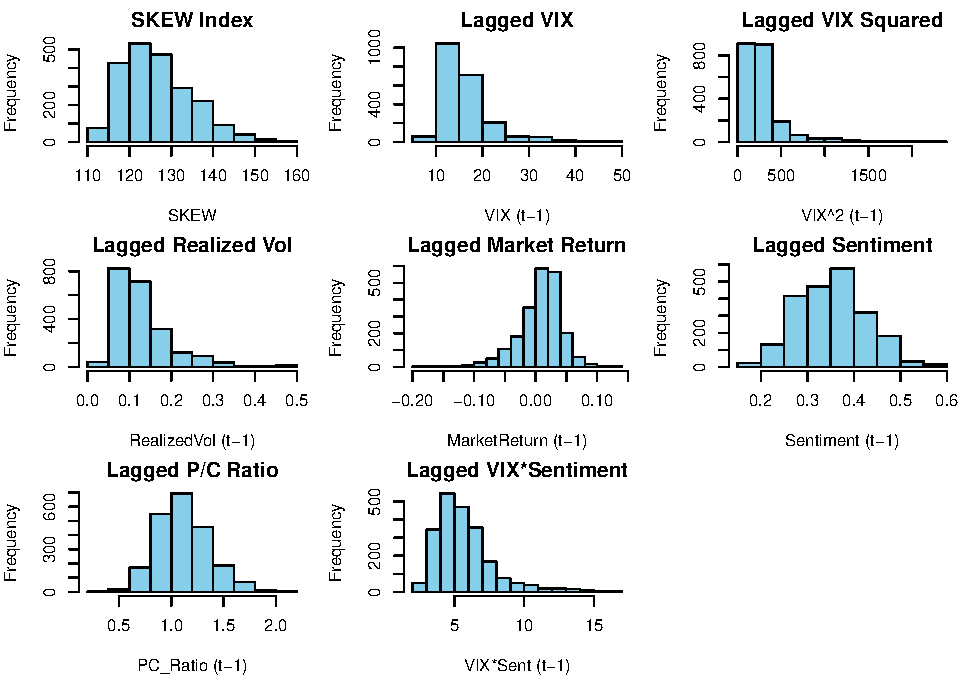
\includegraphics{FinalProject_files/figure-latex/exploratory-data-analysis-1.pdf}

\begin{Shaded}
\begin{Highlighting}[]
  \CommentTok{\#boxplots}
  
  \FunctionTok{par}\NormalTok{(}\AttributeTok{mfrow=}\FunctionTok{c}\NormalTok{(}\DecValTok{3}\NormalTok{,}\DecValTok{3}\NormalTok{), }\AttributeTok{mar=}\FunctionTok{c}\NormalTok{(}\DecValTok{4}\NormalTok{,}\DecValTok{4}\NormalTok{,}\DecValTok{2}\NormalTok{,}\DecValTok{1}\NormalTok{))}
  \FunctionTok{boxplot}\NormalTok{(final\_model\_data}\SpecialCharTok{$}\NormalTok{SKEW, }\AttributeTok{main=}\StringTok{"SKEW Index"}\NormalTok{, }\AttributeTok{col=}\StringTok{"lightgreen"}\NormalTok{)}
  \FunctionTok{boxplot}\NormalTok{(final\_model\_data}\SpecialCharTok{$}\NormalTok{VIX\_lag1, }\AttributeTok{main=}\StringTok{"Lagged VIX"}\NormalTok{, }\AttributeTok{col=}\StringTok{"lightgreen"}\NormalTok{)}
  \FunctionTok{boxplot}\NormalTok{(final\_model\_data}\SpecialCharTok{$}\NormalTok{VIX\_sq\_lag1, }\AttributeTok{main=}\StringTok{"Lagged VIX Squared"}\NormalTok{, }\AttributeTok{col=}\StringTok{"lightgreen"}\NormalTok{)}
  \FunctionTok{boxplot}\NormalTok{(final\_model\_data}\SpecialCharTok{$}\NormalTok{RealizedVol\_lag1, }\AttributeTok{main=}\StringTok{"Lagged Realized Vol"}\NormalTok{, }\AttributeTok{col=}\StringTok{"lightgreen"}\NormalTok{)}
  \FunctionTok{boxplot}\NormalTok{(final\_model\_data}\SpecialCharTok{$}\NormalTok{MarketReturn\_lag1, }\AttributeTok{main=}\StringTok{"Lagged Market Return"}\NormalTok{, }\AttributeTok{col=}\StringTok{"lightgreen"}\NormalTok{)}
  \FunctionTok{boxplot}\NormalTok{(final\_model\_data}\SpecialCharTok{$}\NormalTok{Sentiment\_lag1, }\AttributeTok{main=}\StringTok{"Lagged Sentiment"}\NormalTok{, }\AttributeTok{col=}\StringTok{"lightgreen"}\NormalTok{)}
  \FunctionTok{boxplot}\NormalTok{(final\_model\_data}\SpecialCharTok{$}\NormalTok{PC\_Ratio\_lag1, }\AttributeTok{main=}\StringTok{"Lagged P/C Ratio"}\NormalTok{, }\AttributeTok{col=}\StringTok{"lightgreen"}\NormalTok{)}
  \FunctionTok{boxplot}\NormalTok{(final\_model\_data}\SpecialCharTok{$}\NormalTok{VIX\_Sentiment\_Interaction\_lag1, }\AttributeTok{main=}\StringTok{"Lagged VIX*Sentiment"}\NormalTok{, }\AttributeTok{col=}\StringTok{"lightgreen"}\NormalTok{)}
  \FunctionTok{par}\NormalTok{(}\AttributeTok{mfrow=}\FunctionTok{c}\NormalTok{(}\DecValTok{1}\NormalTok{,}\DecValTok{1}\NormalTok{))}
\end{Highlighting}
\end{Shaded}

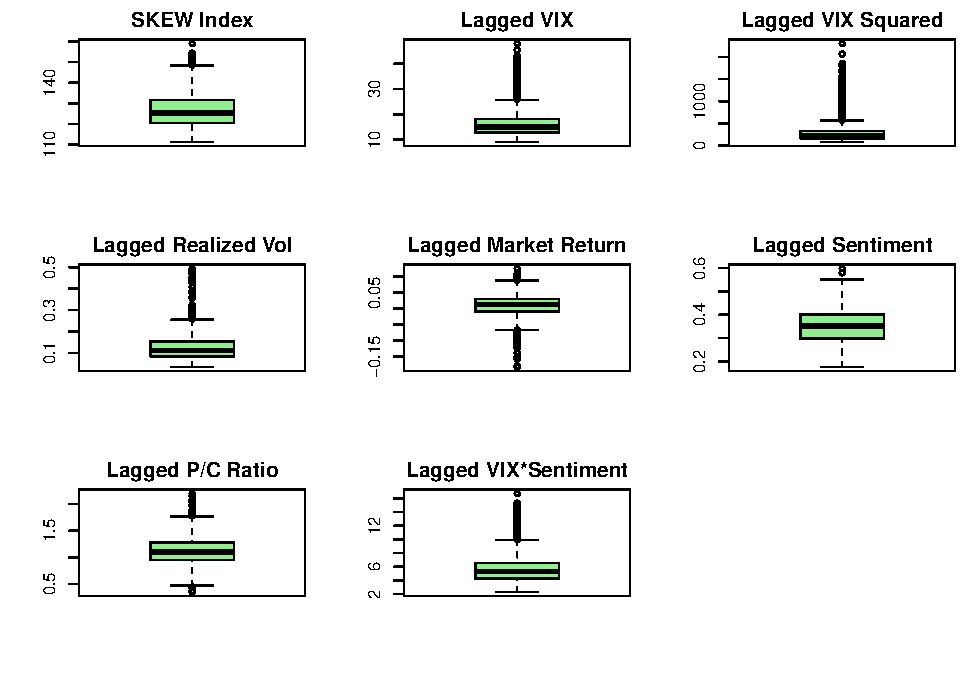
\includegraphics{FinalProject_files/figure-latex/exploratory-data-analysis-2.pdf}

\begin{Shaded}
\begin{Highlighting}[]
  \CommentTok{\#correlation plot}
  
\NormalTok{  numeric\_cols\_for\_corr }\OtherTok{\textless{}{-}}\NormalTok{ final\_model\_data }\SpecialCharTok{\%\textgreater{}\%} \FunctionTok{select}\NormalTok{(}\SpecialCharTok{{-}}\NormalTok{Date)}
\NormalTok{  cor\_matrix\_full }\OtherTok{\textless{}{-}} \FunctionTok{cor}\NormalTok{(numeric\_cols\_for\_corr, }\AttributeTok{use =} \StringTok{"complete.obs"}\NormalTok{)}
  \FunctionTok{corrplot}\NormalTok{(cor\_matrix\_full, }\AttributeTok{method =} \StringTok{"number"}\NormalTok{, }\AttributeTok{type =} \StringTok{"upper"}\NormalTok{, }\AttributeTok{order =} \StringTok{"hclust"}\NormalTok{, }
           \AttributeTok{tl.col =} \StringTok{"black"}\NormalTok{, }\AttributeTok{tl.srt =} \DecValTok{45}\NormalTok{, }\AttributeTok{tl.cex =} \FloatTok{0.7}\NormalTok{, }\AttributeTok{number.cex =} \FloatTok{0.6}\NormalTok{,}
           \AttributeTok{addCoef.col =} \StringTok{"black"}\NormalTok{,}
           \AttributeTok{cl.cex =} \FloatTok{0.7}\NormalTok{)}
  \FunctionTok{title}\NormalTok{(}\StringTok{"Correlation Matrix of Model Variables"}\NormalTok{, }\AttributeTok{line =} \DecValTok{3}\NormalTok{)}
\end{Highlighting}
\end{Shaded}

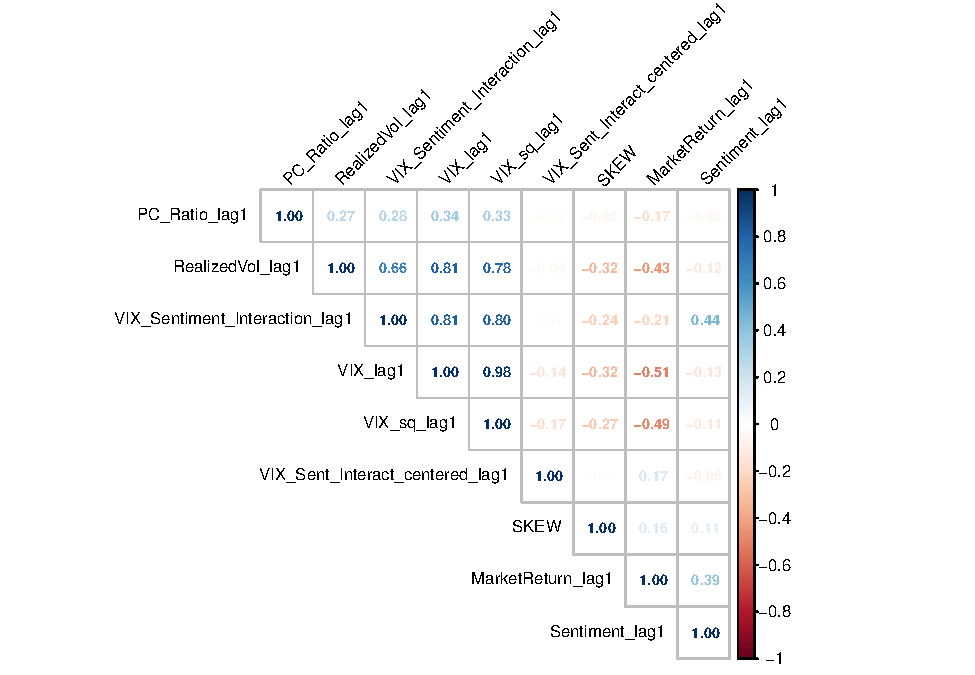
\includegraphics{FinalProject_files/figure-latex/exploratory-data-analysis-3.pdf}

\begin{Shaded}
\begin{Highlighting}[]
\NormalTok{  model1 }\OtherTok{\textless{}{-}} \FunctionTok{lm}\NormalTok{(SKEW }\SpecialCharTok{\textasciitilde{}}\NormalTok{ VIX\_lag1 }\SpecialCharTok{+}\NormalTok{ VIX\_sq\_lag1 }\SpecialCharTok{+}\NormalTok{ RealizedVol\_lag1 }\SpecialCharTok{+} 
\NormalTok{                   MarketReturn\_lag1 }\SpecialCharTok{+}\NormalTok{ Sentiment\_lag1 }\SpecialCharTok{+}\NormalTok{ PC\_Ratio\_lag1 }\SpecialCharTok{+} 
\NormalTok{                   VIX\_Sent\_Interact\_centered\_lag1, }
                 \AttributeTok{data =}\NormalTok{ final\_model\_data)}
  \FunctionTok{summary}\NormalTok{(model1)}
\end{Highlighting}
\end{Shaded}

Call: lm(formula = SKEW \textasciitilde{} VIX\_lag1 + VIX\_sq\_lag1 +
RealizedVol\_lag1 + MarketReturn\_lag1 + Sentiment\_lag1 +
PC\_Ratio\_lag1 + VIX\_Sent\_Interact\_centered\_lag1, data =
final\_model\_data)

Residuals: Min 1Q Median 3Q Max -17.688 -5.342 -1.240 4.349 31.766

Coefficients: Estimate Std. Error t value
Pr(\textgreater\textbar t\textbar)\\
(Intercept) 142.329818 1.750968 81.286 \textless{} 2e-16 \textbf{\emph{
VIX\_lag1 -1.640704 0.148173 -11.073 \textless{} 2e-16 }} VIX\_sq\_lag1
0.029782 0.003104 9.596 \textless{} 2e-16 \textbf{\emph{
RealizedVol\_lag1 -19.189084 4.071824 -4.713 2.6e-06 }}
MarketReturn\_lag1 -11.442986 5.844857 -1.958 0.05038 .\\
Sentiment\_lag1 6.857745 2.392234 2.867 0.00419 ** PC\_Ratio\_lag1
2.183907 0.674255 3.239 0.00122 ** VIX\_Sent\_Interact\_centered\_lag1
-0.125238 0.457637 -0.274 0.78437\\
--- Signif. codes: 0 `\emph{\textbf{' 0.001 '}' 0.01 '}' 0.05 `.' 0.1 '
' 1

Residual standard error: 7.43 on 2157 degrees of freedom Multiple
R-squared: 0.1603, Adjusted R-squared: 0.1575 F-statistic: 58.81 on 7
and 2157 DF, p-value: \textless{} 2.2e-16

\begin{Shaded}
\begin{Highlighting}[]
\NormalTok{  my\_covariate\_labels\_m1\_centered }\OtherTok{\textless{}{-}} \FunctionTok{c}\NormalTok{(}
    \StringTok{"VIX (t{-}1)"}\NormalTok{, }
    \StringTok{"VIX$\^{}\{2\}$ (t{-}1)"}\NormalTok{, }
    \StringTok{"Realized Vol (t{-}1, 21d)"}\NormalTok{, }
    \StringTok{"Market Return (t{-}1, 21d)"}\NormalTok{, }
    \StringTok{"AAII Sentiment (t{-}1, Bullish }\SpecialCharTok{\textbackslash{}\textbackslash{}}\StringTok{\%)"}\NormalTok{,}
    \StringTok{"SPX Put{-}Call Ratio (t{-}1)"}\NormalTok{,}
    \StringTok{"$}\SpecialCharTok{\textbackslash{}\textbackslash{}}\StringTok{text\{VIX\}\_c}\SpecialCharTok{\textbackslash{}\textbackslash{}}\StringTok{ (t}\SpecialCharTok{\textbackslash{}\textbackslash{}}\StringTok{!{-}}\SpecialCharTok{\textbackslash{}\textbackslash{}}\StringTok{!1) }\SpecialCharTok{\textbackslash{}\textbackslash{}}\StringTok{times }\SpecialCharTok{\textbackslash{}\textbackslash{}}\StringTok{text\{Sent\}\_c}\SpecialCharTok{\textbackslash{}\textbackslash{}}\StringTok{ (t}\SpecialCharTok{\textbackslash{}\textbackslash{}}\StringTok{!{-}}\SpecialCharTok{\textbackslash{}\textbackslash{}}\StringTok{!1)$"}
\NormalTok{  )}


  \FunctionTok{stargazer}\NormalTok{(model1, }
            \AttributeTok{type =} \StringTok{"latex"}\NormalTok{,}
            \AttributeTok{title =} \StringTok{"Table 1: OLS Regression for SKEW Index (Centered Interaction)"}\NormalTok{,}
            \AttributeTok{align =} \ConstantTok{TRUE}\NormalTok{, }
            \AttributeTok{dep.var.labels =} \StringTok{"CBOE SKEW Index (Daily)"}\NormalTok{,}
            \AttributeTok{covariate.labels =}\NormalTok{ my\_covariate\_labels\_m1\_centered,}
            \AttributeTok{ci =} \ConstantTok{TRUE}\NormalTok{, }\AttributeTok{ci.level =} \FloatTok{0.95}\NormalTok{, }\AttributeTok{single.row =} \ConstantTok{FALSE}\NormalTok{, }
            \AttributeTok{omit.stat =} \FunctionTok{c}\NormalTok{(}\StringTok{"ser"}\NormalTok{, }\StringTok{"rsq"}\NormalTok{, }\StringTok{"f"}\NormalTok{),}
            \AttributeTok{add.lines =} \FunctionTok{list}\NormalTok{(}
                \FunctionTok{c}\NormalTok{(}\StringTok{"Observations"}\NormalTok{, }\FunctionTok{formatC}\NormalTok{(}\FunctionTok{nobs}\NormalTok{(model1), }\AttributeTok{format=}\StringTok{"d"}\NormalTok{, }\AttributeTok{big.mark=}\StringTok{","}\NormalTok{)),}
                \FunctionTok{c}\NormalTok{(}\StringTok{"R{-}squared"}\NormalTok{, }\FunctionTok{format}\NormalTok{(}\FunctionTok{round}\NormalTok{(}\FunctionTok{summary}\NormalTok{(model1)}\SpecialCharTok{$}\NormalTok{r.squared, }\DecValTok{3}\NormalTok{), }\AttributeTok{nsmall =} \DecValTok{3}\NormalTok{)),}
                \FunctionTok{c}\NormalTok{(}\StringTok{"Adj. R{-}squared"}\NormalTok{, }\FunctionTok{format}\NormalTok{(}\FunctionTok{round}\NormalTok{(}\FunctionTok{summary}\NormalTok{(model1)}\SpecialCharTok{$}\NormalTok{adj.r.squared, }\DecValTok{3}\NormalTok{), }\AttributeTok{nsmall =} \DecValTok{3}\NormalTok{)),}
                \FunctionTok{c}\NormalTok{(}\StringTok{"F{-}statistic"}\NormalTok{, }\FunctionTok{paste0}\NormalTok{(}\FunctionTok{format}\NormalTok{(}\FunctionTok{round}\NormalTok{(}\FunctionTok{summary}\NormalTok{(model1)}\SpecialCharTok{$}\NormalTok{fstatistic[[}\StringTok{"value"}\NormalTok{]],}\DecValTok{2}\NormalTok{),}\AttributeTok{nsmall=}\DecValTok{2}\NormalTok{),}
                                      \FunctionTok{ifelse}\NormalTok{(}\FunctionTok{pf}\NormalTok{(}\FunctionTok{summary}\NormalTok{(model1)}\SpecialCharTok{$}\NormalTok{fstatistic[[}\StringTok{"value"}\NormalTok{]],}
                                                \FunctionTok{summary}\NormalTok{(model1)}\SpecialCharTok{$}\NormalTok{fstatistic[[}\StringTok{"numdf"}\NormalTok{]],}
                                                \FunctionTok{summary}\NormalTok{(model1)}\SpecialCharTok{$}\NormalTok{fstatistic[[}\StringTok{"dendf"}\NormalTok{]],}
                                                \AttributeTok{lower.tail=}\ConstantTok{FALSE}\NormalTok{)}\SpecialCharTok{\textless{}}\FloatTok{0.001}\NormalTok{,}\StringTok{"\^{}\{***\}"}\NormalTok{,}
                                             \FunctionTok{ifelse}\NormalTok{(}\FunctionTok{pf}\NormalTok{(}\FunctionTok{summary}\NormalTok{(model1)}\SpecialCharTok{$}\NormalTok{fstatistic[[}\StringTok{"value"}\NormalTok{]],}
                                                       \FunctionTok{summary}\NormalTok{(model1)}\SpecialCharTok{$}\NormalTok{fstatistic[[}\StringTok{"numdf"}\NormalTok{]],}
                                                       \FunctionTok{summary}\NormalTok{(model1)}\SpecialCharTok{$}\NormalTok{fstatistic[[}\StringTok{"dendf"}\NormalTok{]],}
                                                       \AttributeTok{lower.tail=}\ConstantTok{FALSE}\NormalTok{)}\SpecialCharTok{\textless{}}\FloatTok{0.01}\NormalTok{,}\StringTok{"\^{}\{**\}"}\NormalTok{,}
                                                    \FunctionTok{ifelse}\NormalTok{(}\FunctionTok{pf}\NormalTok{(}\FunctionTok{summary}\NormalTok{(model1)}\SpecialCharTok{$}\NormalTok{fstatistic[[}\StringTok{"value"}\NormalTok{]],}
                                                              \FunctionTok{summary}\NormalTok{(model1)}\SpecialCharTok{$}\NormalTok{fstatistic[[}\StringTok{"numdf"}\NormalTok{]],}
                                                              \FunctionTok{summary}\NormalTok{(model1)}\SpecialCharTok{$}\NormalTok{fstatistic[[}\StringTok{"dendf"}\NormalTok{]],}
                                                              \AttributeTok{lower.tail=}\ConstantTok{FALSE}\NormalTok{)}\SpecialCharTok{\textless{}}\FloatTok{0.05}\NormalTok{,}\StringTok{"\^{}\{*\}"}\NormalTok{, }\StringTok{""}\NormalTok{))),}
                                      \StringTok{" (df = "}\NormalTok{, }\FunctionTok{summary}\NormalTok{(model1)}\SpecialCharTok{$}\NormalTok{fstatistic[[}\StringTok{"numdf"}\NormalTok{]], }\StringTok{", "}\NormalTok{, }\FunctionTok{summary}\NormalTok{(model1)}\SpecialCharTok{$}\NormalTok{fstatistic[[}\StringTok{"dendf"}\NormalTok{]],}\StringTok{")"}\NormalTok{))),}
              \AttributeTok{star.cutoffs =} \FunctionTok{c}\NormalTok{(}\FloatTok{0.05}\NormalTok{, }\FloatTok{0.01}\NormalTok{, }\FloatTok{0.001}\NormalTok{), }
              \AttributeTok{notes =} \FunctionTok{c}\NormalTok{(}\StringTok{"$\^{}\{*\}$p$\textless{}$.05; $\^{}\{**\}$p$\textless{}$.01; $\^{}\{***\}$p$\textless{}$.001. OLS Standard Errors."}\NormalTok{), }
              \AttributeTok{notes.align =} \StringTok{"l"}\NormalTok{, }
              \AttributeTok{notes.append =} \ConstantTok{FALSE}\NormalTok{,}
              \AttributeTok{notes.label =} \StringTok{""}\NormalTok{,}
              \AttributeTok{header =} \ConstantTok{FALSE}\NormalTok{, }
              \AttributeTok{float =} \ConstantTok{FALSE}\NormalTok{, }
              \AttributeTok{no.space =} \ConstantTok{TRUE}\NormalTok{, }
              \AttributeTok{font.size =} \StringTok{"small"}\NormalTok{,}
              \AttributeTok{digits =} \DecValTok{3}
\NormalTok{      )}
\end{Highlighting}
\end{Shaded}

\begingroup 
\small 
\begin{tabular}{@{\extracolsep{5pt}}lD{.}{.}{-3} } 
\\[-1.8ex]\hline 
\hline \\[-1.8ex] 
 & \multicolumn{1}{c}{\textit{Dependent variable:}} \\ 
\cline{2-2} 
\\[-1.8ex] & \multicolumn{1}{c}{CBOE SKEW Index (Daily)} \\ 
\hline \\[-1.8ex] 
 VIX (t-1) & -1.641^{***} \\ 
  & \multicolumn{1}{c}{(-1.931$, $-1.350)} \\ 
  VIX$^{2}$ (t-1) & 0.030^{***} \\ 
  & \multicolumn{1}{c}{(0.024$, $0.036)} \\ 
  Realized Vol (t-1, 21d) & -19.189^{***} \\ 
  & \multicolumn{1}{c}{(-27.170$, $-11.208)} \\ 
  Market Return (t-1, 21d) & -11.443 \\ 
  & \multicolumn{1}{c}{(-22.899$, $0.013)} \\ 
  AAII Sentiment (t-1, Bullish \%) & 6.858^{**} \\ 
  & \multicolumn{1}{c}{(2.169$, $11.546)} \\ 
  SPX Put-Call Ratio (t-1) & 2.184^{**} \\ 
  & \multicolumn{1}{c}{(0.862$, $3.505)} \\ 
  $\text{VIX}_c\ (t\!-\!1) \times \text{Sent}_c\ (t\!-\!1)$ & -0.125 \\ 
  & \multicolumn{1}{c}{(-1.022$, $0.772)} \\ 
  Constant & 142.330^{***} \\ 
  & \multicolumn{1}{c}{(138.898$, $145.762)} \\ 
 \hline \\[-1.8ex] 
Observations & 2,165 \\ 
R-squared & 0.160 \\ 
Adj. R-squared & 0.158 \\ 
F-statistic & 58.81^{***} (df = 7, 2157) \\ 
Observations & \multicolumn{1}{c}{2,165} \\ 
Adjusted R$^{2}$ & \multicolumn{1}{c}{0.158} \\ 
\hline 
\hline \\[-1.8ex] 
\multicolumn{2}{l}{$^{*}$p$<$.05; $^{**}$p$<$.01; $^{***}$p$<$.001. OLS Standard Errors.} \\ 
\end{tabular} 
\endgroup

\begin{Shaded}
\begin{Highlighting}[]
  \FunctionTok{par}\NormalTok{(}\AttributeTok{mfrow=}\FunctionTok{c}\NormalTok{(}\DecValTok{2}\NormalTok{,}\DecValTok{2}\NormalTok{)) }
  \FunctionTok{plot}\NormalTok{(model1) }
\end{Highlighting}
\end{Shaded}

\begin{figure}
\centering
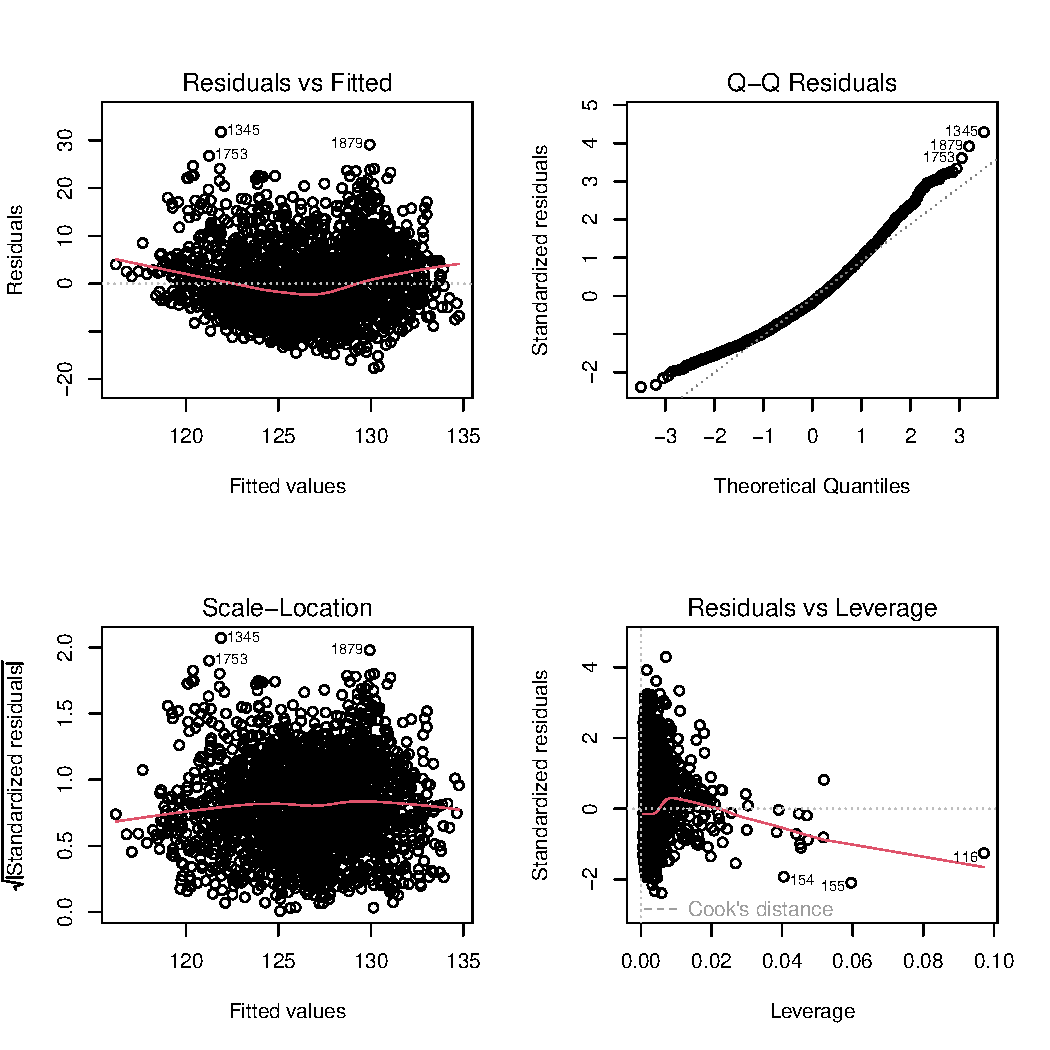
\includegraphics{FinalProject_files/figure-latex/model1-diagnostics-1.pdf}
\caption{Regression Diagnostic Plots for OLS Model}
\end{figure}

\begin{Shaded}
\begin{Highlighting}[]
  \FunctionTok{par}\NormalTok{(}\AttributeTok{mfrow=}\FunctionTok{c}\NormalTok{(}\DecValTok{1}\NormalTok{,}\DecValTok{1}\NormalTok{))}
  
  \FunctionTok{crPlots}\NormalTok{(model1, }
        \AttributeTok{terms =} \SpecialCharTok{\textasciitilde{}}\NormalTok{ ., }
        \AttributeTok{layout =} \ConstantTok{NULL}\NormalTok{, }
        \AttributeTok{ask =} \ConstantTok{FALSE}\NormalTok{, }
        \AttributeTok{smooth =} \FunctionTok{list}\NormalTok{(}\AttributeTok{smoother =}\NormalTok{ loessLine, }\AttributeTok{col.lines =} \StringTok{"blue"}\NormalTok{),}
        \AttributeTok{col =} \StringTok{"black"}\NormalTok{,}
        \AttributeTok{pch =} \DecValTok{19}\NormalTok{,      }
        \AttributeTok{cex =} \FloatTok{0.7}\NormalTok{,}
        \AttributeTok{main=}\StringTok{"Component+Residual Plots (Model 1)"}\NormalTok{)     }
\end{Highlighting}
\end{Shaded}

\begin{figure}
\centering
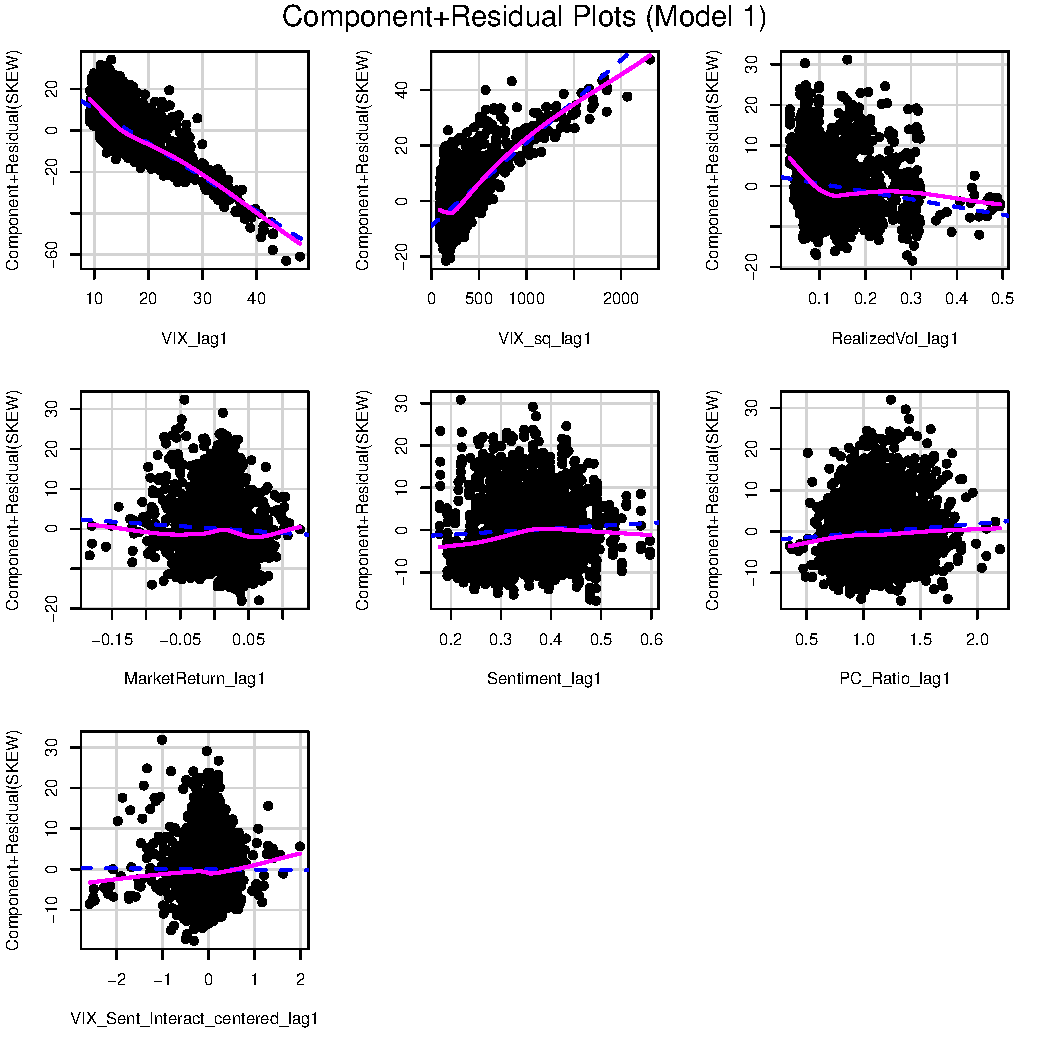
\includegraphics{FinalProject_files/figure-latex/model1-diagnostics-2.pdf}
\caption{Regression Diagnostic Plots for OLS Model}
\end{figure}

\begin{Shaded}
\begin{Highlighting}[]
  \FunctionTok{print}\NormalTok{(}\StringTok{"{-}{-}{-} Normality of Residuals {-}{-}{-}"}\NormalTok{)}
\end{Highlighting}
\end{Shaded}

{[}1{]} ``--- Normality of Residuals ---''

\begin{Shaded}
\begin{Highlighting}[]
\NormalTok{  shapiro\_test\_result }\OtherTok{\textless{}{-}} \FunctionTok{shapiro.test}\NormalTok{(}\FunctionTok{residuals}\NormalTok{(model1))}
  \FunctionTok{print}\NormalTok{(shapiro\_test\_result)}
\end{Highlighting}
\end{Shaded}

\begin{verbatim}
Shapiro-Wilk normality test
\end{verbatim}

data: residuals(model1) W = 0.96534, p-value \textless{} 2.2e-16

\begin{Shaded}
\begin{Highlighting}[]
  \FunctionTok{hist}\NormalTok{(}\FunctionTok{residuals}\NormalTok{(model1), }\AttributeTok{main=}\StringTok{"Histogram of Residuals"}\NormalTok{, }\AttributeTok{xlab=}\StringTok{"Residuals"}\NormalTok{, }\AttributeTok{breaks=}\DecValTok{50}\NormalTok{, }\AttributeTok{col=}\StringTok{"lightblue"}\NormalTok{)}
\end{Highlighting}
\end{Shaded}

\begin{figure}
\centering
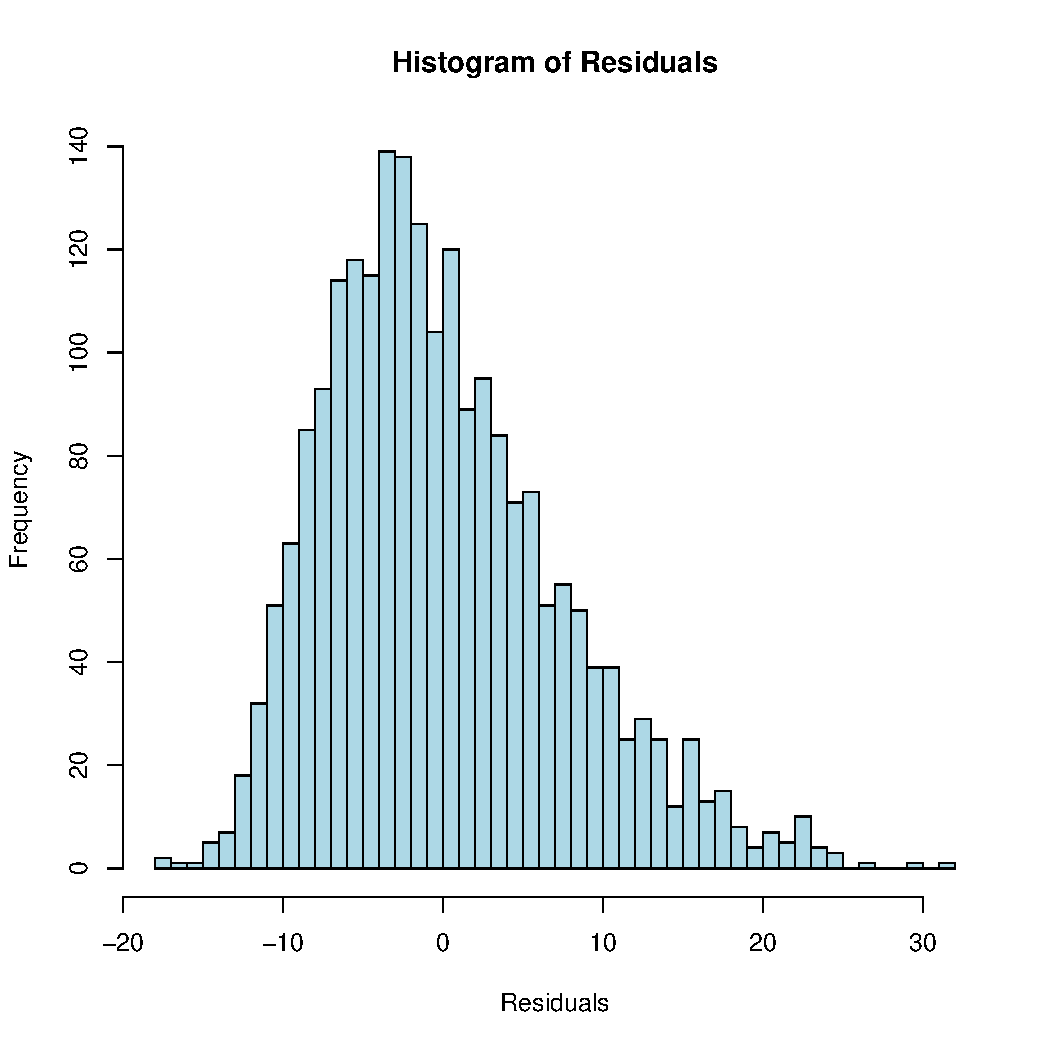
\includegraphics{FinalProject_files/figure-latex/model1-diagnostics-3.pdf}
\caption{Regression Diagnostic Plots for OLS Model}
\end{figure}

\begin{Shaded}
\begin{Highlighting}[]
  \FunctionTok{print}\NormalTok{(}\FunctionTok{paste}\NormalTok{(}\StringTok{"Skewness of residuals:"}\NormalTok{, }\FunctionTok{skewness}\NormalTok{(}\FunctionTok{residuals}\NormalTok{(model1))))}
\end{Highlighting}
\end{Shaded}

{[}1{]} ``Skewness of residuals: 0.744755613212608''

\begin{Shaded}
\begin{Highlighting}[]
  \FunctionTok{print}\NormalTok{(}\FunctionTok{paste}\NormalTok{(}\StringTok{"Kurtosis of residuals (excess kurtosis):"}\NormalTok{, }\FunctionTok{kurtosis}\NormalTok{(}\FunctionTok{residuals}\NormalTok{(model1)) }\SpecialCharTok{{-}} \DecValTok{3}\NormalTok{))}
\end{Highlighting}
\end{Shaded}

{[}1{]} ``Kurtosis of residuals (excess kurtosis): 0.45261610468358''

\begin{Shaded}
\begin{Highlighting}[]
  \FunctionTok{print}\NormalTok{(}\StringTok{"{-}{-}{-} Homoscedasticity {-}{-}{-}"}\NormalTok{)}
\end{Highlighting}
\end{Shaded}

{[}1{]} ``--- Homoscedasticity ---''

\begin{Shaded}
\begin{Highlighting}[]
\NormalTok{  bp\_test\_result }\OtherTok{\textless{}{-}} \FunctionTok{bptest}\NormalTok{(model1, }\AttributeTok{studentize =} \ConstantTok{FALSE}\NormalTok{)}
  \FunctionTok{print}\NormalTok{(bp\_test\_result)}
\end{Highlighting}
\end{Shaded}

\begin{verbatim}
Breusch-Pagan test
\end{verbatim}

data: model1 BP = 58.866, df = 7, p-value = 2.541e-10

\begin{Shaded}
\begin{Highlighting}[]
  \FunctionTok{print}\NormalTok{(}\StringTok{"{-}{-}{-} Autocorrelation of Residuals {-}{-}{-}"}\NormalTok{)}
\end{Highlighting}
\end{Shaded}

{[}1{]} ``--- Autocorrelation of Residuals ---''

\begin{Shaded}
\begin{Highlighting}[]
\NormalTok{  dw\_test\_result }\OtherTok{\textless{}{-}} \FunctionTok{dwtest}\NormalTok{(model1)}
  \FunctionTok{print}\NormalTok{(dw\_test\_result)}
\end{Highlighting}
\end{Shaded}

\begin{verbatim}
Durbin-Watson test
\end{verbatim}

data: model1 DW = 0.27423, p-value \textless{} 2.2e-16 alternative
hypothesis: true autocorrelation is greater than 0

\begin{Shaded}
\begin{Highlighting}[]
  \FunctionTok{par}\NormalTok{(}\AttributeTok{mfrow=}\FunctionTok{c}\NormalTok{(}\DecValTok{1}\NormalTok{,}\DecValTok{2}\NormalTok{))}
  \FunctionTok{acf}\NormalTok{(}\FunctionTok{residuals}\NormalTok{(model1), }\AttributeTok{main=}\StringTok{"ACF of Residuals"}\NormalTok{)}
  \FunctionTok{pacf}\NormalTok{(}\FunctionTok{residuals}\NormalTok{(model1), }\AttributeTok{main=}\StringTok{"PACF of Residuals"}\NormalTok{)}
\end{Highlighting}
\end{Shaded}

\begin{figure}
\centering
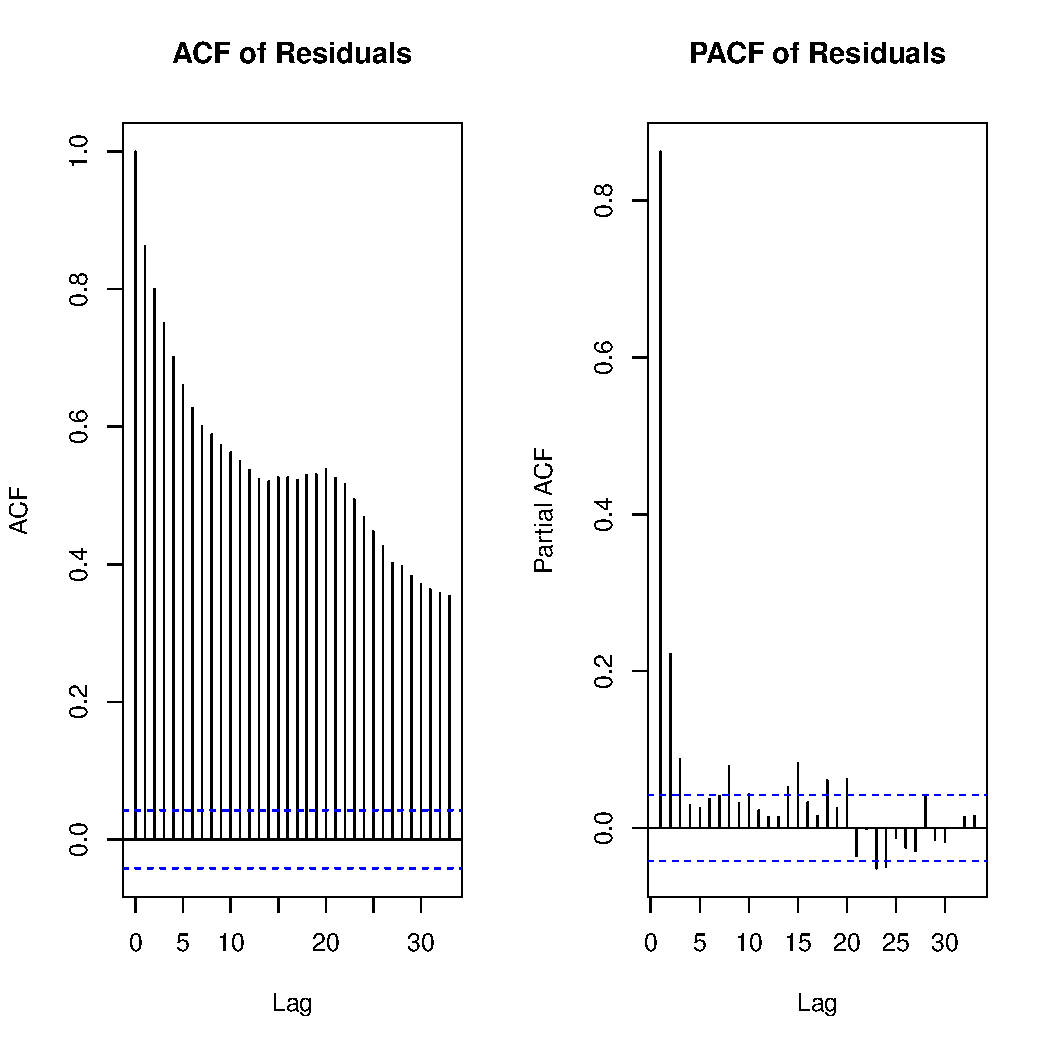
\includegraphics{FinalProject_files/figure-latex/model1-diagnostics-4.pdf}
\caption{Regression Diagnostic Plots for OLS Model}
\end{figure}

\begin{Shaded}
\begin{Highlighting}[]
  \FunctionTok{par}\NormalTok{(}\AttributeTok{mfrow=}\FunctionTok{c}\NormalTok{(}\DecValTok{1}\NormalTok{,}\DecValTok{1}\NormalTok{))}
\NormalTok{  ljung\_box\_test\_10 }\OtherTok{\textless{}{-}} \FunctionTok{Box.test}\NormalTok{(}\FunctionTok{residuals}\NormalTok{(model1), }\AttributeTok{lag =} \DecValTok{10}\NormalTok{, }\AttributeTok{type =} \StringTok{"Ljung{-}Box"}\NormalTok{)}
\NormalTok{  ljung\_box\_test\_20 }\OtherTok{\textless{}{-}} \FunctionTok{Box.test}\NormalTok{(}\FunctionTok{residuals}\NormalTok{(model1), }\AttributeTok{lag =} \DecValTok{20}\NormalTok{, }\AttributeTok{type =} \StringTok{"Ljung{-}Box"}\NormalTok{)}
  \FunctionTok{print}\NormalTok{(}\StringTok{"Ljung{-}Box test for autocorrelation (10 lags):"}\NormalTok{)}
\end{Highlighting}
\end{Shaded}

{[}1{]} ``Ljung-Box test for autocorrelation (10 lags):''

\begin{Shaded}
\begin{Highlighting}[]
  \FunctionTok{print}\NormalTok{(ljung\_box\_test\_10)}
\end{Highlighting}
\end{Shaded}

\begin{verbatim}
Box-Ljung test
\end{verbatim}

data: residuals(model1) X-squared = 10035, df = 10, p-value \textless{}
2.2e-16

\begin{Shaded}
\begin{Highlighting}[]
  \FunctionTok{print}\NormalTok{(}\StringTok{"Ljung{-}Box test for autocorrelation (20 lags):"}\NormalTok{)}
\end{Highlighting}
\end{Shaded}

{[}1{]} ``Ljung-Box test for autocorrelation (20 lags):''

\begin{Shaded}
\begin{Highlighting}[]
  \FunctionTok{print}\NormalTok{(ljung\_box\_test\_20)}
\end{Highlighting}
\end{Shaded}

\begin{verbatim}
Box-Ljung test
\end{verbatim}

data: residuals(model1) X-squared = 16182, df = 20, p-value \textless{}
2.2e-16

\begin{Shaded}
\begin{Highlighting}[]
  \FunctionTok{print}\NormalTok{(}\StringTok{"{-}{-}{-} Multicollinearity {-}{-}{-}"}\NormalTok{)}
\end{Highlighting}
\end{Shaded}

{[}1{]} ``--- Multicollinearity ---''

\begin{Shaded}
\begin{Highlighting}[]
\NormalTok{  vif\_values }\OtherTok{\textless{}{-}} \FunctionTok{vif}\NormalTok{(model1)}
  \FunctionTok{print}\NormalTok{(vif\_values)}
\end{Highlighting}
\end{Shaded}

\begin{verbatim}
                   VIX_lag1                     VIX_sq_lag1 
                  25.064134                       21.865569 
           RealizedVol_lag1               MarketReturn_lag1 
                   3.011822                        1.621272 
             Sentiment_lag1                   PC_Ratio_lag1 
                   1.209796                        1.134291 
\end{verbatim}

VIX\_Sent\_Interact\_centered\_lag1 1.110096

\begin{Shaded}
\begin{Highlighting}[]
  \FunctionTok{print}\NormalTok{(}\StringTok{"{-}{-}{-} Outliers and Influential Points {-}{-}{-}"}\NormalTok{)}
\end{Highlighting}
\end{Shaded}

{[}1{]} ``--- Outliers and Influential Points ---''

\begin{Shaded}
\begin{Highlighting}[]
\NormalTok{  cooksd }\OtherTok{\textless{}{-}} \FunctionTok{cooks.distance}\NormalTok{(model1)}
  \FunctionTok{plot}\NormalTok{(cooksd, }\AttributeTok{pch=}\StringTok{"*"}\NormalTok{, }\AttributeTok{cex=}\DecValTok{1}\NormalTok{, }\AttributeTok{main=}\StringTok{"Cook\textquotesingle{}s Distance Plot"}\NormalTok{, }\AttributeTok{ylab=}\StringTok{"Cook\textquotesingle{}s Distance"}\NormalTok{)}
  \FunctionTok{abline}\NormalTok{(}\AttributeTok{h =} \DecValTok{4}\SpecialCharTok{/}\FunctionTok{nobs}\NormalTok{(model1), }\AttributeTok{col=}\StringTok{"red"}\NormalTok{, }\AttributeTok{lty=}\DecValTok{2}\NormalTok{)}
\end{Highlighting}
\end{Shaded}

\begin{figure}
\centering
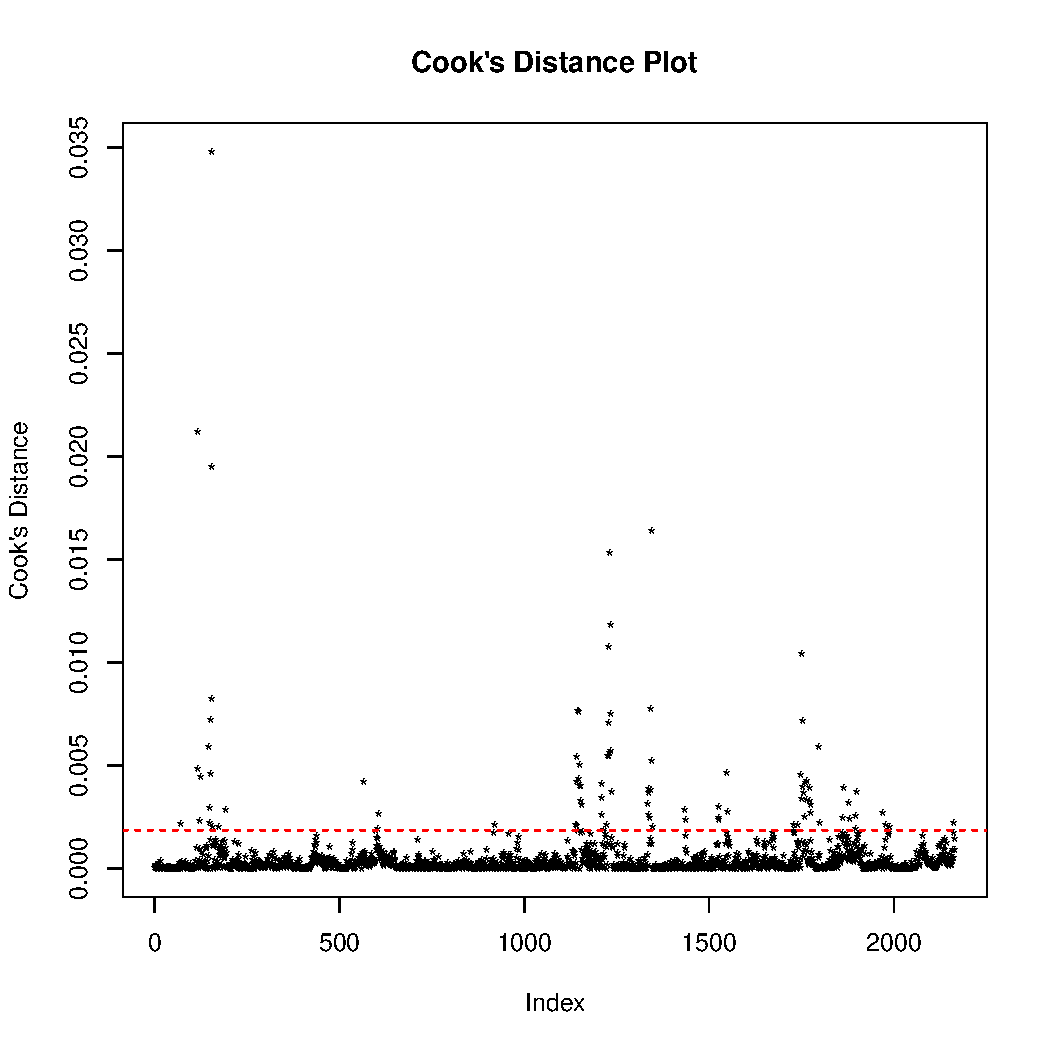
\includegraphics{FinalProject_files/figure-latex/model1-diagnostics-5.pdf}
\caption{Regression Diagnostic Plots for OLS Model}
\end{figure}

\begin{Shaded}
\begin{Highlighting}[]
\NormalTok{  influential\_threshold\_4\_n }\OtherTok{\textless{}{-}} \DecValTok{4}\SpecialCharTok{/}\FunctionTok{nobs}\NormalTok{(model1)}
\NormalTok{  influential\_points\_4\_n }\OtherTok{\textless{}{-}} \FunctionTok{which}\NormalTok{(cooksd }\SpecialCharTok{\textgreater{}}\NormalTok{ influential\_threshold\_4\_n)}
  \FunctionTok{print}\NormalTok{(}\FunctionTok{paste}\NormalTok{(}\StringTok{"Number of points with Cook\textquotesingle{}s D \textgreater{} 4/n:"}\NormalTok{, }\FunctionTok{length}\NormalTok{(influential\_points\_4\_n)))}
\end{Highlighting}
\end{Shaded}

{[}1{]} ``Number of points with Cook's D \textgreater{} 4/n: 94''

\begin{Shaded}
\begin{Highlighting}[]
  \ControlFlowTok{if}\NormalTok{(}\FunctionTok{length}\NormalTok{(influential\_points\_4\_n) }\SpecialCharTok{\textgreater{}} \DecValTok{0} \SpecialCharTok{\&\&} \FunctionTok{length}\NormalTok{(influential\_points\_4\_n) }\SpecialCharTok{\textless{}} \DecValTok{20}\NormalTok{) \{}
      \FunctionTok{print}\NormalTok{(}\FunctionTok{paste}\NormalTok{(}\StringTok{"Indices of points with Cook\textquotesingle{}s D \textgreater{} 4/n:"}\NormalTok{, }\FunctionTok{paste}\NormalTok{(}\FunctionTok{head}\NormalTok{(influential\_points\_4\_n, }\DecValTok{10}\NormalTok{), }\AttributeTok{collapse=}\StringTok{", "}\NormalTok{)))}
\NormalTok{  \}}
\NormalTok{  influential\_points\_1 }\OtherTok{\textless{}{-}} \FunctionTok{which}\NormalTok{(cooksd }\SpecialCharTok{\textgreater{}} \DecValTok{1}\NormalTok{)}
  \FunctionTok{print}\NormalTok{(}\FunctionTok{paste}\NormalTok{(}\StringTok{"Number of points with Cook\textquotesingle{}s D \textgreater{} 1:"}\NormalTok{, }\FunctionTok{length}\NormalTok{(influential\_points\_1)))}
\end{Highlighting}
\end{Shaded}

{[}1{]} ``Number of points with Cook's D \textgreater{} 1: 0''

\begin{Shaded}
\begin{Highlighting}[]
  \ControlFlowTok{if}\NormalTok{(}\FunctionTok{length}\NormalTok{(influential\_points\_1) }\SpecialCharTok{\textgreater{}} \DecValTok{0}\NormalTok{) \{}
      \FunctionTok{print}\NormalTok{(}\FunctionTok{paste}\NormalTok{(}\StringTok{"Indices of points with Cook\textquotesingle{}s D \textgreater{} 1:"}\NormalTok{, }\FunctionTok{paste}\NormalTok{(influential\_points\_1, }\AttributeTok{collapse=}\StringTok{", "}\NormalTok{)))}
\NormalTok{  \}}
    
\NormalTok{  residuals\_df\_m1 }\OtherTok{\textless{}{-}} \FunctionTok{data.frame}\NormalTok{(}\AttributeTok{Date =}\NormalTok{ final\_model\_data}\SpecialCharTok{$}\NormalTok{Date, }\AttributeTok{Residuals =} \FunctionTok{residuals}\NormalTok{(model1))}
\NormalTok{  p\_res\_time\_m1 }\OtherTok{\textless{}{-}} \FunctionTok{ggplot}\NormalTok{(residuals\_df\_m1, }\FunctionTok{aes}\NormalTok{(}\AttributeTok{x =}\NormalTok{ Date, }\AttributeTok{y =}\NormalTok{ Residuals)) }\SpecialCharTok{+}
    \FunctionTok{geom\_line}\NormalTok{(}\AttributeTok{color =} \StringTok{"steelblue"}\NormalTok{) }\SpecialCharTok{+} \FunctionTok{geom\_hline}\NormalTok{(}\AttributeTok{yintercept =} \DecValTok{0}\NormalTok{, }\AttributeTok{linetype =} \StringTok{"dashed"}\NormalTok{, }\AttributeTok{color =} \StringTok{"red"}\NormalTok{) }\SpecialCharTok{+}
    \FunctionTok{labs}\NormalTok{(}\AttributeTok{title =} \StringTok{"Model 1 Residuals vs. Time"}\NormalTok{, }\AttributeTok{x =} \StringTok{"Date"}\NormalTok{, }\AttributeTok{y =} \StringTok{"Residuals"}\NormalTok{) }\SpecialCharTok{+} \FunctionTok{theme\_minimal}\NormalTok{()}
  \FunctionTok{print}\NormalTok{(p\_res\_time\_m1)}
\end{Highlighting}
\end{Shaded}

\begin{figure}
\centering
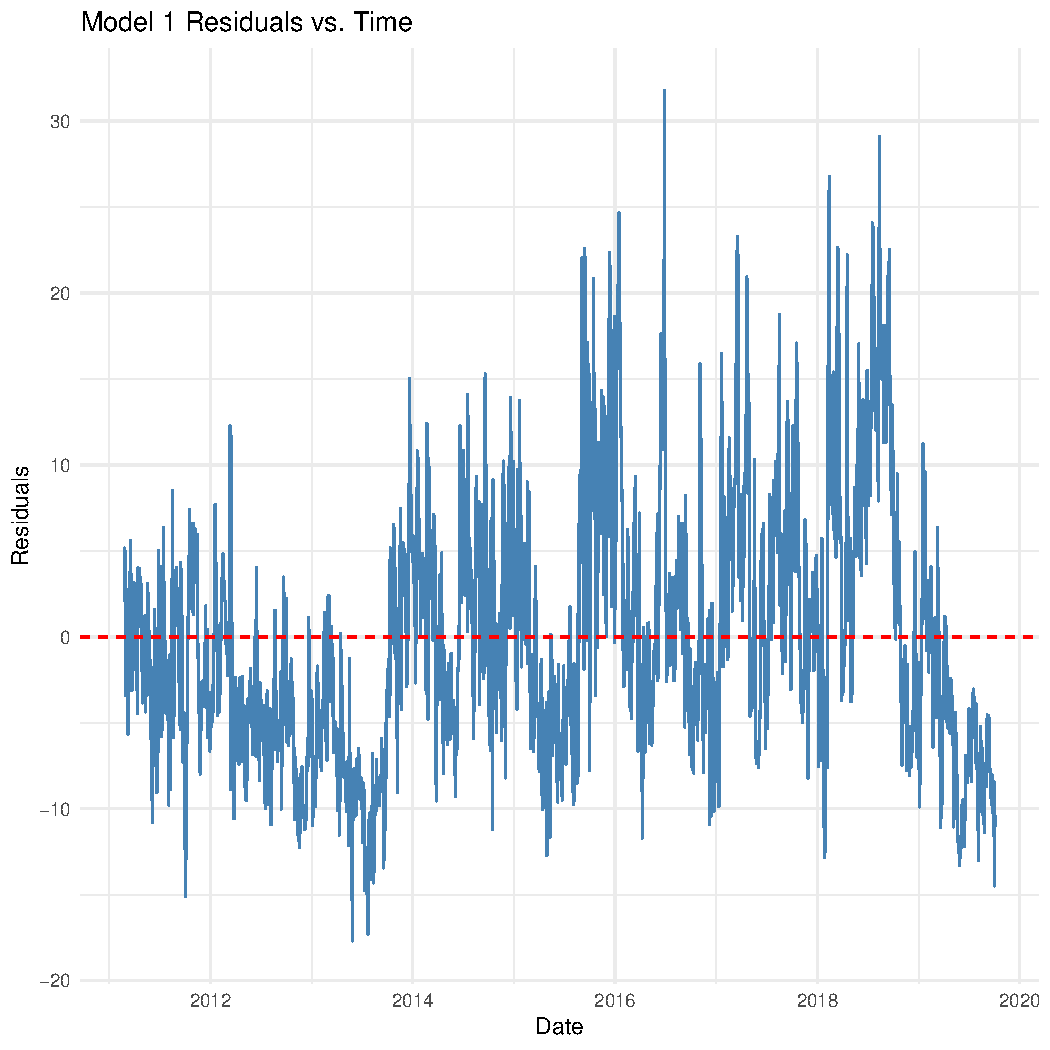
\includegraphics{FinalProject_files/figure-latex/model1-diagnostics-6.pdf}
\caption{Regression Diagnostic Plots for OLS Model}
\end{figure}

\begin{Shaded}
\begin{Highlighting}[]
\NormalTok{  nw\_lag\_m1 }\OtherTok{\textless{}{-}} \FunctionTok{floor}\NormalTok{(}\DecValTok{4}\SpecialCharTok{*}\NormalTok{(}\FunctionTok{nobs}\NormalTok{(model1)}\SpecialCharTok{/}\DecValTok{100}\NormalTok{)}\SpecialCharTok{\^{}}\NormalTok{(}\DecValTok{2}\SpecialCharTok{/}\DecValTok{9}\NormalTok{)) }
\NormalTok{  model1\_hac\_summary }\OtherTok{\textless{}{-}} \FunctionTok{coeftest}\NormalTok{(model1, }\AttributeTok{vcov. =} \FunctionTok{NeweyWest}\NormalTok{(model1, }\AttributeTok{lag =}\NormalTok{ nw\_lag\_m1, }\AttributeTok{prewhite =} \ConstantTok{FALSE}\NormalTok{, }\AttributeTok{adjust =} \ConstantTok{TRUE}\NormalTok{))}
  
  \FunctionTok{stargazer}\NormalTok{(model1, }
            \AttributeTok{type =} \StringTok{"latex"}\NormalTok{,}
            \AttributeTok{title =} \StringTok{"Table 2: SKEW Index Regression with Newey{-}West HAC SEs (Model 1)"}\NormalTok{,}
            \AttributeTok{align =} \ConstantTok{TRUE}\NormalTok{, }
            \AttributeTok{dep.var.labels =} \StringTok{"CBOE SKEW Index (Daily)"}\NormalTok{,}
            \AttributeTok{covariate.labels =}\NormalTok{ my\_covariate\_labels\_m1\_centered, }
            \AttributeTok{coef =} \FunctionTok{list}\NormalTok{(}\FunctionTok{coef}\NormalTok{(model1)),}
            \AttributeTok{se =} \FunctionTok{list}\NormalTok{(model1\_hac\_summary[, }\StringTok{"Std. Error"}\NormalTok{]),}
            \AttributeTok{t =} \FunctionTok{list}\NormalTok{(model1\_hac\_summary[, }\StringTok{"t value"}\NormalTok{]),}
            \AttributeTok{p =} \FunctionTok{list}\NormalTok{(model1\_hac\_summary[, }\StringTok{"Pr(\textgreater{}|t|)"}\NormalTok{]),}
            \AttributeTok{omit.stat =} \FunctionTok{c}\NormalTok{(}\StringTok{"ser"}\NormalTok{, }\StringTok{"rsq"}\NormalTok{, }\StringTok{"f"}\NormalTok{, }\StringTok{"adj.rsq"}\NormalTok{), }
            \AttributeTok{add.lines =} \FunctionTok{list}\NormalTok{(}
                \FunctionTok{c}\NormalTok{(}\StringTok{"Observations"}\NormalTok{, }\FunctionTok{formatC}\NormalTok{(}\FunctionTok{nobs}\NormalTok{(model1), }\AttributeTok{format=}\StringTok{"d"}\NormalTok{, }\AttributeTok{big.mark=}\StringTok{","}\NormalTok{)),}
                \FunctionTok{c}\NormalTok{(}\StringTok{"R{-}squared (OLS)"}\NormalTok{, }\FunctionTok{format}\NormalTok{(}\FunctionTok{round}\NormalTok{(}\FunctionTok{summary}\NormalTok{(model1)}\SpecialCharTok{$}\NormalTok{r.squared, }\DecValTok{3}\NormalTok{), }\AttributeTok{nsmall =} \DecValTok{3}\NormalTok{)),}
                \FunctionTok{c}\NormalTok{(}\StringTok{"Adj. R{-}squared (OLS)"}\NormalTok{, }\FunctionTok{format}\NormalTok{(}\FunctionTok{round}\NormalTok{(}\FunctionTok{summary}\NormalTok{(model1)}\SpecialCharTok{$}\NormalTok{adj.r.squared, }\DecValTok{3}\NormalTok{), }\AttributeTok{nsmall =} \DecValTok{3}\NormalTok{)),}
                \FunctionTok{c}\NormalTok{(}\StringTok{"Newey{-}West Lag Chosen"}\NormalTok{, nw\_lag\_m1),}
                \FunctionTok{c}\NormalTok{(}\StringTok{"Durbin{-}Watson Stat. (OLS)"}\NormalTok{, }\FunctionTok{format}\NormalTok{(}\FunctionTok{round}\NormalTok{(}\FunctionTok{dwtest}\NormalTok{(model1)}\SpecialCharTok{$}\NormalTok{statistic,}\DecValTok{2}\NormalTok{),}\AttributeTok{nsmall=}\DecValTok{2}\NormalTok{))}
\NormalTok{            ),}
            \AttributeTok{star.cutoffs =} \FunctionTok{c}\NormalTok{(}\FloatTok{0.05}\NormalTok{, }\FloatTok{0.01}\NormalTok{, }\FloatTok{0.001}\NormalTok{), }
            \AttributeTok{notes =} \StringTok{"$\^{}\{*\}$p$\textless{}$.05; $\^{}\{**\}$p$\textless{}$.01; $\^{}\{***\}$p$\textless{}$.001. Newey{-}West HAC Standard Errors."}\NormalTok{,}
            \AttributeTok{notes.align =} \StringTok{"l"}\NormalTok{, }\AttributeTok{notes.append =} \ConstantTok{FALSE}\NormalTok{, }\AttributeTok{notes.label =} \StringTok{""}\NormalTok{,    }
            \AttributeTok{header =} \ConstantTok{FALSE}\NormalTok{, }\AttributeTok{float =} \ConstantTok{FALSE}\NormalTok{, }\AttributeTok{no.space =} \ConstantTok{TRUE}\NormalTok{, }\AttributeTok{font.size =} \StringTok{"small"}\NormalTok{,}
            \AttributeTok{digits =} \DecValTok{3}
\NormalTok{  )}
\end{Highlighting}
\end{Shaded}

\begingroup 
\small 
\begin{tabular}{@{\extracolsep{5pt}}lD{.}{.}{-3} } 
\\[-1.8ex]\hline 
\hline \\[-1.8ex] 
 & \multicolumn{1}{c}{\textit{Dependent variable:}} \\ 
\cline{2-2} 
\\[-1.8ex] & \multicolumn{1}{c}{CBOE SKEW Index (Daily)} \\ 
\hline \\[-1.8ex] 
 VIX (t-1) & -1.641^{***} \\ 
  & (0.308) \\ 
  VIX$^{2}$ (t-1) & 0.030^{***} \\ 
  & (0.007) \\ 
  Realized Vol (t-1, 21d) & -19.189^{*} \\ 
  & (9.353) \\ 
  Market Return (t-1, 21d) & -11.443 \\ 
  & (11.445) \\ 
  AAII Sentiment (t-1, Bullish \%) & 6.858 \\ 
  & (5.337) \\ 
  SPX Put-Call Ratio (t-1) & 2.184^{*} \\ 
  & (0.980) \\ 
  $\text{VIX}_c\ (t\!-\!1) \times \text{Sent}_c\ (t\!-\!1)$ & -0.125 \\ 
  & (1.034) \\ 
  Constant & 142.330^{***} \\ 
  & (3.344) \\ 
 \hline \\[-1.8ex] 
Observations & 2,165 \\ 
R-squared (OLS) & 0.160 \\ 
Adj. R-squared (OLS) & 0.158 \\ 
Newey-West Lag Chosen & 7 \\ 
Durbin-Watson Stat. (OLS) & 0.27 \\ 
Observations & \multicolumn{1}{c}{2,165} \\ 
\hline 
\hline \\[-1.8ex] 
\multicolumn{2}{l}{$^{*}$p$<$.05; $^{**}$p$<$.01; $^{***}$p$<$.001. Newey-West HAC Standard Errors.} \\ 
\end{tabular} 
\endgroup

\begin{Shaded}
\begin{Highlighting}[]
\NormalTok{  final\_model\_data\_log }\OtherTok{\textless{}{-}}\NormalTok{ final\_model\_data }\SpecialCharTok{\%\textgreater{}\%}
  \FunctionTok{filter}\NormalTok{(SKEW }\SpecialCharTok{\textgreater{}} \DecValTok{0} \SpecialCharTok{\&}\NormalTok{ VIX\_lag1 }\SpecialCharTok{\textgreater{}} \DecValTok{0} \SpecialCharTok{\&}\NormalTok{ RealizedVol\_lag1 }\SpecialCharTok{\textgreater{}} \DecValTok{0} \SpecialCharTok{\&}\NormalTok{ PC\_Ratio\_lag1 }\SpecialCharTok{\textgreater{}} \DecValTok{0} \SpecialCharTok{\&}\NormalTok{ Sentiment\_lag1 }\SpecialCharTok{\textgreater{}} \DecValTok{0}\NormalTok{) }
  
\NormalTok{  final\_model\_data\_log }\OtherTok{\textless{}{-}}\NormalTok{ final\_model\_data\_log }\SpecialCharTok{\%\textgreater{}\%}
    \FunctionTok{mutate}\NormalTok{(}
      \AttributeTok{log\_SKEW =} \FunctionTok{log}\NormalTok{(SKEW),}
      \AttributeTok{log\_VIX\_lag1 =} \FunctionTok{log}\NormalTok{(VIX\_lag1),}
      \AttributeTok{log\_RealizedVol\_lag1 =} \FunctionTok{log}\NormalTok{(RealizedVol\_lag1),}
      \AttributeTok{log\_PC\_Ratio\_lag1 =} \FunctionTok{log}\NormalTok{(PC\_Ratio\_lag1),}
      \AttributeTok{log\_Sentiment\_lag1 =} \FunctionTok{log}\NormalTok{(Sentiment\_lag1) }
\NormalTok{    ) }\SpecialCharTok{\%\textgreater{}\%}
    \FunctionTok{mutate}\NormalTok{(}
      \AttributeTok{log\_VIX\_lag1\_centered\_logmodel =}\NormalTok{ log\_VIX\_lag1 }\SpecialCharTok{{-}} \FunctionTok{mean}\NormalTok{(log\_VIX\_lag1, }\AttributeTok{na.rm=}\ConstantTok{TRUE}\NormalTok{),}
      \AttributeTok{log\_Sentiment\_lag1\_centered\_logmodel =}\NormalTok{ log\_Sentiment\_lag1 }\SpecialCharTok{{-}} \FunctionTok{mean}\NormalTok{(log\_Sentiment\_lag1, }\AttributeTok{na.rm=}\ConstantTok{TRUE}\NormalTok{),}
      \AttributeTok{logVIX\_logSent\_Interact\_centered\_lag1 =}\NormalTok{ log\_VIX\_lag1\_centered\_logmodel }\SpecialCharTok{*}\NormalTok{ log\_Sentiment\_lag1\_centered\_logmodel}
\NormalTok{    )}
  
\NormalTok{    model2\_log }\OtherTok{\textless{}{-}} \FunctionTok{lm}\NormalTok{(log\_SKEW }\SpecialCharTok{\textasciitilde{}}\NormalTok{ log\_VIX\_lag1 }\SpecialCharTok{+}\NormalTok{ log\_RealizedVol\_lag1 }\SpecialCharTok{+} 
\NormalTok{                           MarketReturn\_lag1 }\SpecialCharTok{+}\NormalTok{ log\_Sentiment\_lag1 }\SpecialCharTok{+}\NormalTok{ log\_PC\_Ratio\_lag1 }\SpecialCharTok{+}
\NormalTok{                           logVIX\_logSent\_Interact\_centered\_lag1, }
                         \AttributeTok{data =}\NormalTok{ final\_model\_data\_log)}
    
\NormalTok{    my\_covariate\_labels\_m2\_log }\OtherTok{\textless{}{-}} \FunctionTok{c}\NormalTok{(}
    \StringTok{"log(VIX (t{-}1))"}\NormalTok{, }
    \StringTok{"log(RealizedVol (t{-}1))"}\NormalTok{, }
    \StringTok{"Market Return (t{-}1)"}\NormalTok{, }
    \StringTok{"log(Sentiment (t{-}1))"}\NormalTok{, }
    \StringTok{"log(P/C Ratio (t{-}1))"}\NormalTok{,}
    \StringTok{"$}\SpecialCharTok{\textbackslash{}\textbackslash{}}\StringTok{log(}\SpecialCharTok{\textbackslash{}\textbackslash{}}\StringTok{text\{VIX\}\_c}\SpecialCharTok{\textbackslash{}\textbackslash{}}\StringTok{ (t\{{-}\}1)) }\SpecialCharTok{\textbackslash{}\textbackslash{}}\StringTok{times }\SpecialCharTok{\textbackslash{}\textbackslash{}}\StringTok{log(}\SpecialCharTok{\textbackslash{}\textbackslash{}}\StringTok{text\{Sent\}\_c}\SpecialCharTok{\textbackslash{}\textbackslash{}}\StringTok{ (t\{{-}\}1))$"}
\NormalTok{  )}

    \FunctionTok{stargazer}\NormalTok{(model2\_log, }
              \AttributeTok{type =} \StringTok{"latex"}\NormalTok{,}
              \AttributeTok{title =} \StringTok{"Table 3: OLS Regression for log(SKEW) (Model 2)"}\NormalTok{,}
              \AttributeTok{align =} \ConstantTok{TRUE}\NormalTok{, }
              \AttributeTok{dep.var.labels =} \StringTok{"log(CBOE SKEW Index)"}\NormalTok{,}
              \AttributeTok{covariate.labels =}\NormalTok{ my\_covariate\_labels\_m2\_log,}
              \AttributeTok{ci =} \ConstantTok{TRUE}\NormalTok{, }\AttributeTok{ci.level=}\FloatTok{0.95}\NormalTok{, }\AttributeTok{single.row=}\ConstantTok{FALSE}\NormalTok{,}
              \AttributeTok{omit.stat=}\FunctionTok{c}\NormalTok{(}\StringTok{"ser"}\NormalTok{,}\StringTok{"rsq"}\NormalTok{,}\StringTok{"f"}\NormalTok{),}
              \AttributeTok{add.lines =} \FunctionTok{list}\NormalTok{(}
                  \FunctionTok{c}\NormalTok{(}\StringTok{"Observations"}\NormalTok{, }\FunctionTok{formatC}\NormalTok{(}\FunctionTok{nobs}\NormalTok{(model2\_log), }\AttributeTok{format=}\StringTok{"d"}\NormalTok{, }\AttributeTok{big.mark=}\StringTok{","}\NormalTok{)),}
                  \FunctionTok{c}\NormalTok{(}\StringTok{"R{-}squared"}\NormalTok{, }\FunctionTok{format}\NormalTok{(}\FunctionTok{round}\NormalTok{(}\FunctionTok{summary}\NormalTok{(model2\_log)}\SpecialCharTok{$}\NormalTok{r.squared,}\DecValTok{3}\NormalTok{),}\AttributeTok{nsmall=}\DecValTok{3}\NormalTok{)),}
                  \FunctionTok{c}\NormalTok{(}\StringTok{"Adj. R{-}squared"}\NormalTok{, }\FunctionTok{format}\NormalTok{(}\FunctionTok{round}\NormalTok{(}\FunctionTok{summary}\NormalTok{(model2\_log)}\SpecialCharTok{$}\NormalTok{adj.r.squared,}\DecValTok{3}\NormalTok{),}\AttributeTok{nsmall=}\DecValTok{3}\NormalTok{)),}
                  \FunctionTok{c}\NormalTok{(}\StringTok{"F{-}statistic"}\NormalTok{, }\FunctionTok{paste0}\NormalTok{(}\FunctionTok{format}\NormalTok{(}\FunctionTok{round}\NormalTok{(}\FunctionTok{summary}\NormalTok{(model2\_log)}\SpecialCharTok{$}\NormalTok{fstatistic[[}\StringTok{"value"}\NormalTok{]],}\DecValTok{2}\NormalTok{),}\AttributeTok{nsmall=}\DecValTok{2}\NormalTok{),}
                                      \FunctionTok{ifelse}\NormalTok{(}\FunctionTok{pf}\NormalTok{(}\FunctionTok{summary}\NormalTok{(model2\_log)}\SpecialCharTok{$}\NormalTok{fstatistic[[}\StringTok{"value"}\NormalTok{]],}
                                                \FunctionTok{summary}\NormalTok{(model2\_log)}\SpecialCharTok{$}\NormalTok{fstatistic[[}\StringTok{"numdf"}\NormalTok{]],}
                                                \FunctionTok{summary}\NormalTok{(model2\_log)}\SpecialCharTok{$}\NormalTok{fstatistic[[}\StringTok{"dendf"}\NormalTok{]],}
                                                \AttributeTok{lower.tail=}\ConstantTok{FALSE}\NormalTok{)}\SpecialCharTok{\textless{}}\FloatTok{0.001}\NormalTok{,}\StringTok{"\^{}\{***\}"}\NormalTok{,}
                                             \FunctionTok{ifelse}\NormalTok{(}\FunctionTok{pf}\NormalTok{(}\FunctionTok{summary}\NormalTok{(model2\_log)}\SpecialCharTok{$}\NormalTok{fstatistic[[}\StringTok{"value"}\NormalTok{]],}
                                                       \FunctionTok{summary}\NormalTok{(model2\_log)}\SpecialCharTok{$}\NormalTok{fstatistic[[}\StringTok{"numdf"}\NormalTok{]],}
                                                       \FunctionTok{summary}\NormalTok{(model2\_log)}\SpecialCharTok{$}\NormalTok{fstatistic[[}\StringTok{"dendf"}\NormalTok{]],}
                                                       \AttributeTok{lower.tail=}\ConstantTok{FALSE}\NormalTok{)}\SpecialCharTok{\textless{}}\FloatTok{0.01}\NormalTok{,}\StringTok{"\^{}\{**\}"}\NormalTok{,}
                                                    \FunctionTok{ifelse}\NormalTok{(}\FunctionTok{pf}\NormalTok{(}\FunctionTok{summary}\NormalTok{(model2\_log)}\SpecialCharTok{$}\NormalTok{fstatistic[[}\StringTok{"value"}\NormalTok{]],}
                                                              \FunctionTok{summary}\NormalTok{(model2\_log)}\SpecialCharTok{$}\NormalTok{fstatistic[[}\StringTok{"numdf"}\NormalTok{]],}
                                                              \FunctionTok{summary}\NormalTok{(model2\_log)}\SpecialCharTok{$}\NormalTok{fstatistic[[}\StringTok{"dendf"}\NormalTok{]],}
                                                              \AttributeTok{lower.tail=}\ConstantTok{FALSE}\NormalTok{)}\SpecialCharTok{\textless{}}\FloatTok{0.05}\NormalTok{,}\StringTok{"\^{}\{*\}"}\NormalTok{, }\StringTok{""}\NormalTok{))),}
                                      \StringTok{" (df = "}\NormalTok{, }\FunctionTok{summary}\NormalTok{(model2\_log)}\SpecialCharTok{$}\NormalTok{fstatistic[[}\StringTok{"numdf"}\NormalTok{]], }\StringTok{", "}\NormalTok{, }\FunctionTok{summary}\NormalTok{(model2\_log)}\SpecialCharTok{$}\NormalTok{fstatistic[[}\StringTok{"dendf"}\NormalTok{]],}\StringTok{")"}\NormalTok{))}
\NormalTok{              ),}
              \AttributeTok{star.cutoffs =} \FunctionTok{c}\NormalTok{(}\FloatTok{0.05}\NormalTok{, }\FloatTok{0.01}\NormalTok{, }\FloatTok{0.001}\NormalTok{), }
              \AttributeTok{notes =} \StringTok{"$\^{}\{*\}$p$\textless{}$.05; $\^{}\{**\}$p$\textless{}$.01; $\^{}\{***\}$p$\textless{}$.001. OLS Standard Errors."}\NormalTok{,}
              \AttributeTok{notes.align=}\StringTok{"l"}\NormalTok{, }\AttributeTok{notes.append=}\ConstantTok{FALSE}\NormalTok{, }\AttributeTok{notes.label=}\StringTok{""}\NormalTok{,    }
              \AttributeTok{header=}\ConstantTok{FALSE}\NormalTok{, }\AttributeTok{float=}\ConstantTok{FALSE}\NormalTok{, }\AttributeTok{no.space=}\ConstantTok{TRUE}\NormalTok{, }\AttributeTok{font.size=}\StringTok{"small"}\NormalTok{,}
              \AttributeTok{digits =} \DecValTok{3}
\NormalTok{    )}
\end{Highlighting}
\end{Shaded}

\begingroup 
\small 
\begin{tabular}{@{\extracolsep{5pt}}lD{.}{.}{-3} } 
\\[-1.8ex]\hline 
\hline \\[-1.8ex] 
 & \multicolumn{1}{c}{\textit{Dependent variable:}} \\ 
\cline{2-2} 
\\[-1.8ex] & \multicolumn{1}{c}{log(CBOE SKEW Index)} \\ 
\hline \\[-1.8ex] 
 log(VIX (t-1)) & -0.043^{***} \\ 
  & \multicolumn{1}{c}{(-0.058$, $-0.028)} \\ 
  log(RealizedVol (t-1)) & -0.038^{***} \\ 
  & \multicolumn{1}{c}{(-0.046$, $-0.029)} \\ 
  Market Return (t-1) & -0.093^{*} \\ 
  & \multicolumn{1}{c}{(-0.181$, $-0.006)} \\ 
  log(Sentiment (t-1)) & 0.020^{**} \\ 
  & \multicolumn{1}{c}{(0.008$, $0.032)} \\ 
  log(P/C Ratio (t-1)) & 0.020^{***} \\ 
  & \multicolumn{1}{c}{(0.008$, $0.031)} \\ 
  $\log(\text{VIX}_c\ (t{-}1)) \times \log(\text{Sent}_c\ (t{-}1))$ & -0.044^{*} \\ 
  & \multicolumn{1}{c}{(-0.086$, $-0.002)} \\ 
  Constant & 4.897^{***} \\ 
  & \multicolumn{1}{c}{(4.837$, $4.957)} \\ 
 \hline \\[-1.8ex] 
Observations & 2,165 \\ 
R-squared & 0.179 \\ 
Adj. R-squared & 0.177 \\ 
F-statistic & 78.51^{***} (df = 6, 2158) \\ 
Observations & \multicolumn{1}{c}{2,165} \\ 
Adjusted R$^{2}$ & \multicolumn{1}{c}{0.177} \\ 
\hline 
\hline \\[-1.8ex] 
\multicolumn{2}{l}{$^{*}$p$<$.05; $^{**}$p$<$.01; $^{***}$p$<$.001. OLS Standard Errors.} \\ 
\end{tabular} 
\endgroup

\begin{Shaded}
\begin{Highlighting}[]
  \FunctionTok{par}\NormalTok{(}\AttributeTok{mfrow=}\FunctionTok{c}\NormalTok{(}\DecValTok{2}\NormalTok{,}\DecValTok{2}\NormalTok{)); }\FunctionTok{plot}\NormalTok{(model2\_log); }\FunctionTok{par}\NormalTok{(}\AttributeTok{mfrow=}\FunctionTok{c}\NormalTok{(}\DecValTok{1}\NormalTok{,}\DecValTok{1}\NormalTok{))}
\end{Highlighting}
\end{Shaded}

\begin{figure}
\centering
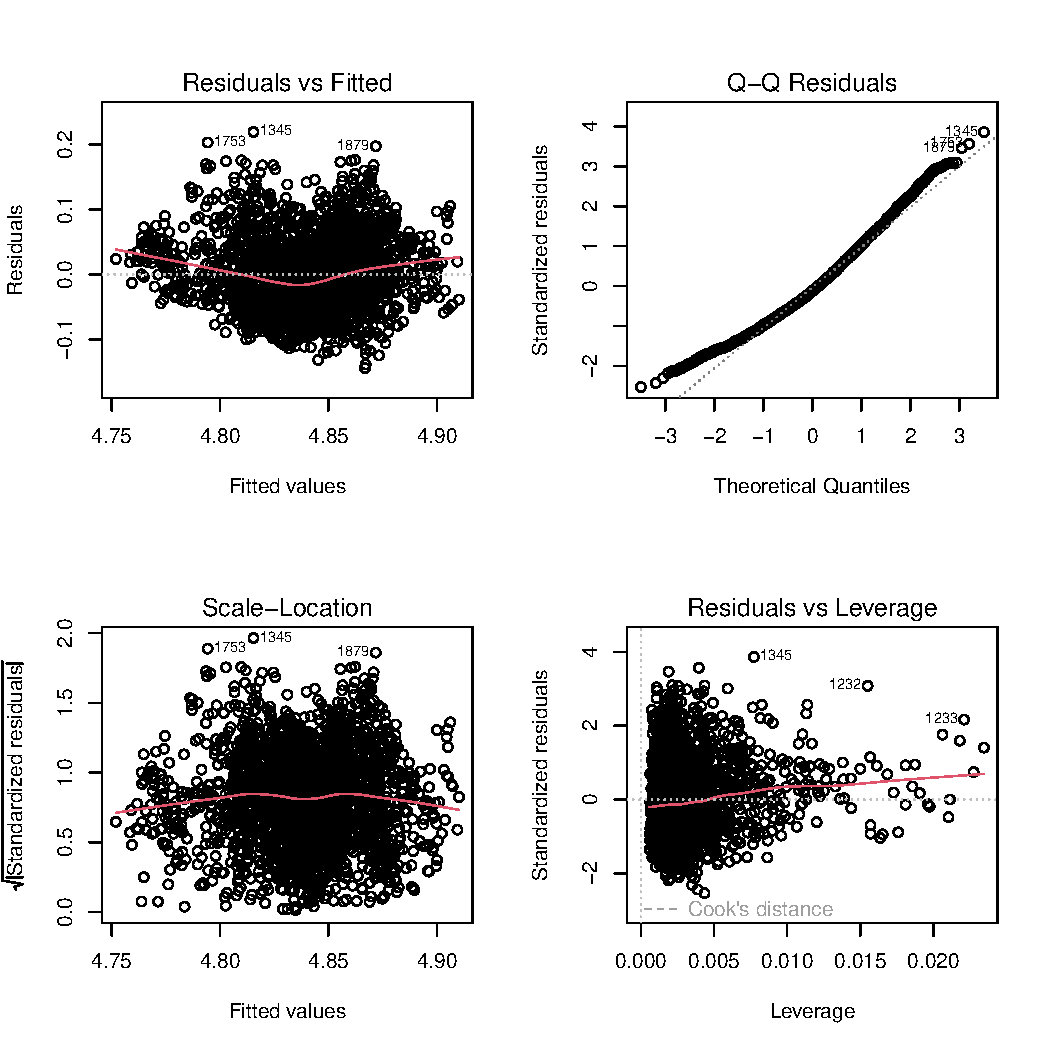
\includegraphics{FinalProject_files/figure-latex/model2-diagnostics-1.pdf}
\caption{Regression Diagnostic Plots for Log Transformed Model}
\end{figure}

\begin{Shaded}
\begin{Highlighting}[]
\NormalTok{    crPlots\_m2\_output }\OtherTok{\textless{}{-}} \FunctionTok{crPlots}\NormalTok{(model2\_log,}
                                 \AttributeTok{terms=} \SpecialCharTok{\textasciitilde{}}\NormalTok{ .,}
                                 \AttributeTok{layout=}\ConstantTok{NULL}\NormalTok{,}
                                 \AttributeTok{ask=}\ConstantTok{FALSE}\NormalTok{,}
                                 \AttributeTok{smooth=}\FunctionTok{list}\NormalTok{(}\AttributeTok{smoother=}\NormalTok{loessLine,}
                                             \AttributeTok{col.lines=}\StringTok{"red"}\NormalTok{,}
                                             \AttributeTok{spread=}\ConstantTok{FALSE}\NormalTok{),}
                                 \AttributeTok{col=}\StringTok{"darkgray"}\NormalTok{,}
                                 \AttributeTok{pch=}\DecValTok{1}\NormalTok{,}
                                 \AttributeTok{cex=}\FloatTok{0.7}\NormalTok{,}
                                 \AttributeTok{main=}\StringTok{"Component+Residual Plots (Model 2)"}\NormalTok{)}
\end{Highlighting}
\end{Shaded}

\begin{figure}
\centering
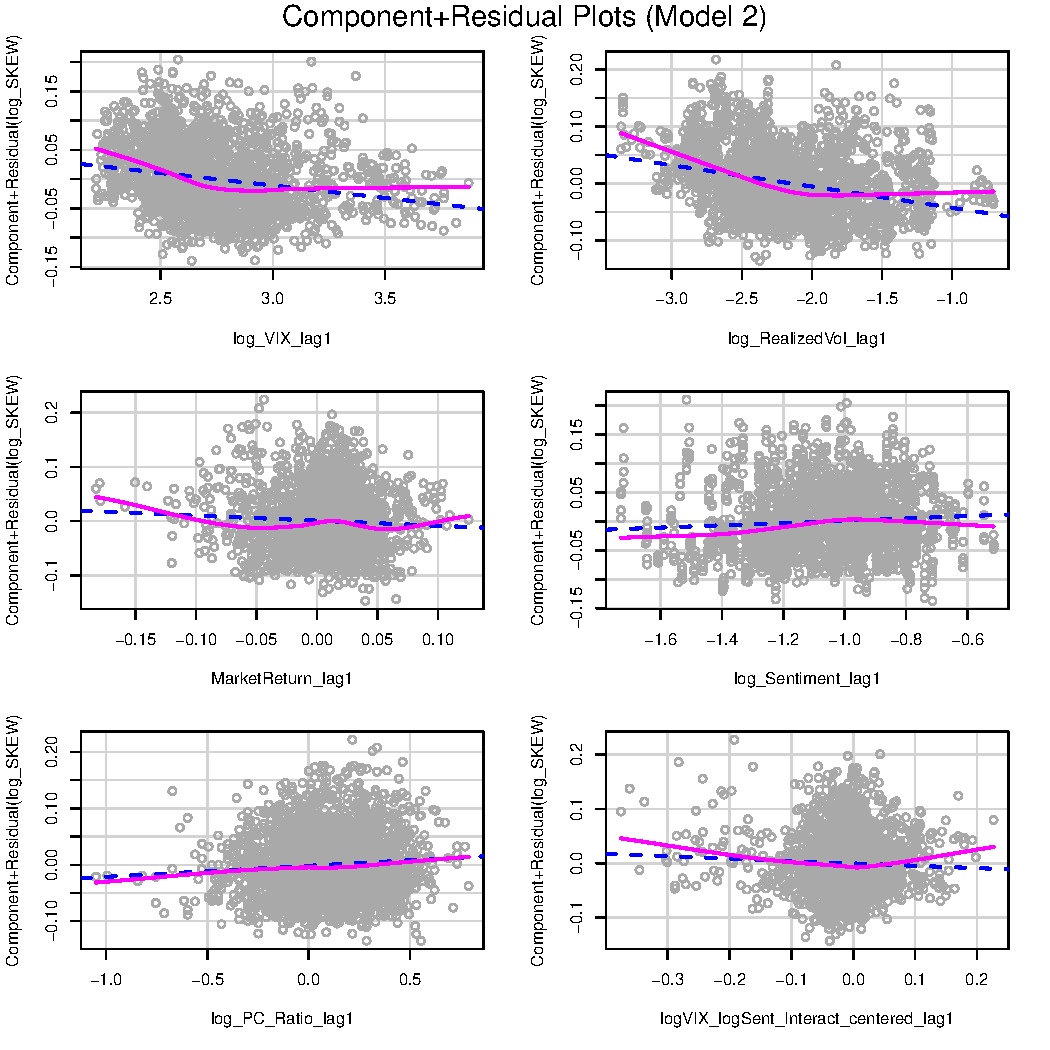
\includegraphics{FinalProject_files/figure-latex/model2-diagnostics-2.pdf}
\caption{Regression Diagnostic Plots for Log Transformed Model}
\end{figure}

\begin{Shaded}
\begin{Highlighting}[]
\NormalTok{    shapiro\_test\_m2 }\OtherTok{\textless{}{-}} \FunctionTok{shapiro.test}\NormalTok{(}\FunctionTok{residuals}\NormalTok{(model2\_log))}
    \FunctionTok{hist}\NormalTok{(}\FunctionTok{residuals}\NormalTok{(model2\_log), }\AttributeTok{breaks=}\DecValTok{50}\NormalTok{, }\AttributeTok{main=}\StringTok{"Residuals Histogram (Model 2)"}\NormalTok{, }\AttributeTok{col=}\StringTok{"lightcoral"}\NormalTok{)}
\end{Highlighting}
\end{Shaded}

\begin{figure}
\centering
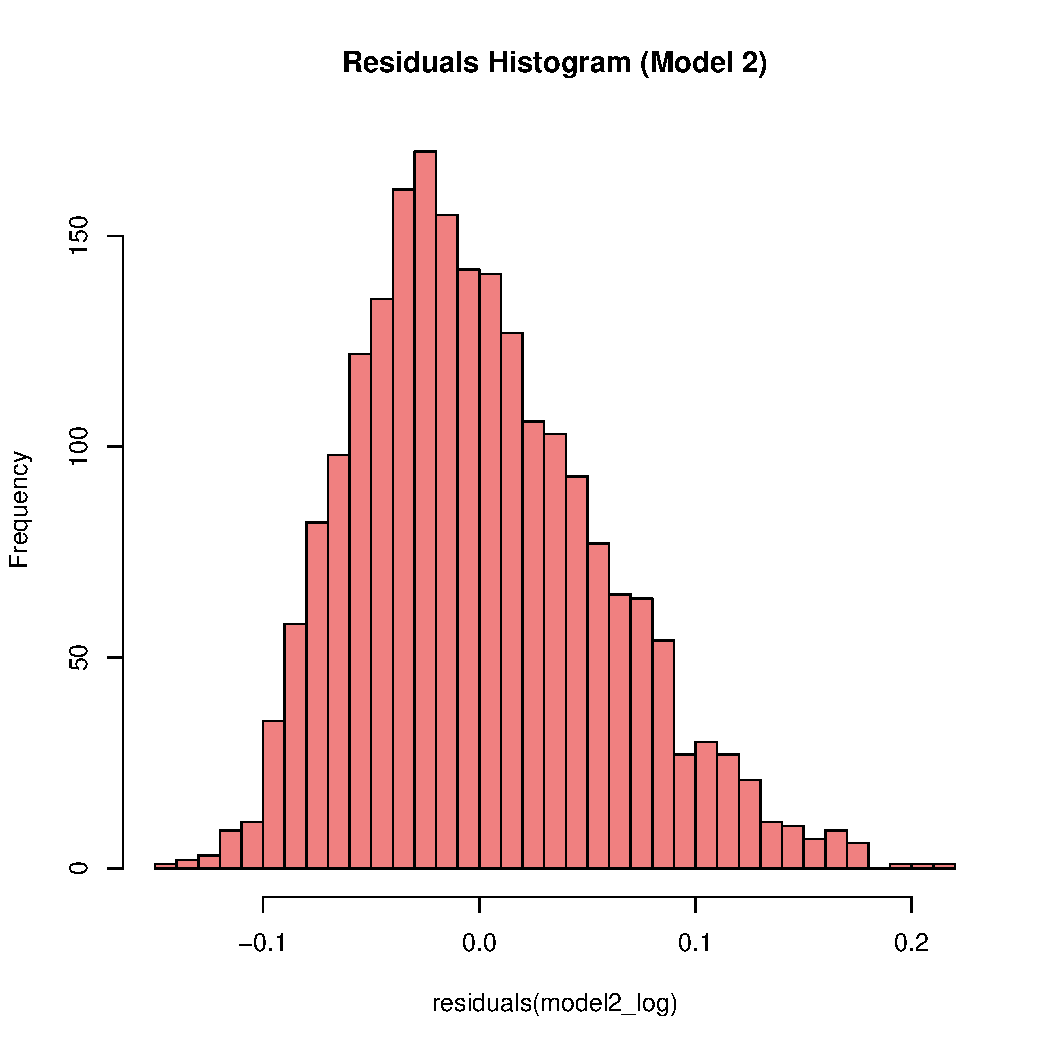
\includegraphics{FinalProject_files/figure-latex/model2-diagnostics-3.pdf}
\caption{Regression Diagnostic Plots for Log Transformed Model}
\end{figure}

\begin{Shaded}
\begin{Highlighting}[]
\NormalTok{    skewness\_m2\_res }\OtherTok{\textless{}{-}} \FunctionTok{skewness}\NormalTok{(}\FunctionTok{residuals}\NormalTok{(model2\_log))}
\NormalTok{    kurtosis\_m2\_res }\OtherTok{\textless{}{-}} \FunctionTok{kurtosis}\NormalTok{(}\FunctionTok{residuals}\NormalTok{(model2\_log))}\SpecialCharTok{{-}}\DecValTok{3}
    
\NormalTok{    bp\_test\_m2 }\OtherTok{\textless{}{-}} \FunctionTok{bptest}\NormalTok{(model2\_log, }\AttributeTok{studentize=}\ConstantTok{FALSE}\NormalTok{)}
    
\NormalTok{    dw\_test\_m2 }\OtherTok{\textless{}{-}} \FunctionTok{dwtest}\NormalTok{(model2\_log)}
    \FunctionTok{par}\NormalTok{(}\AttributeTok{mfrow=}\FunctionTok{c}\NormalTok{(}\DecValTok{1}\NormalTok{,}\DecValTok{2}\NormalTok{)); }\FunctionTok{acf}\NormalTok{(}\FunctionTok{residuals}\NormalTok{(model2\_log), }\AttributeTok{main=}\StringTok{"ACF Residuals (Model 2)"}\NormalTok{); }\FunctionTok{pacf}\NormalTok{(}\FunctionTok{residuals}\NormalTok{(model2\_log), }\AttributeTok{main=}\StringTok{"PACF Residuals (Model 2)"}\NormalTok{); }\FunctionTok{par}\NormalTok{(}\AttributeTok{mfrow=}\FunctionTok{c}\NormalTok{(}\DecValTok{1}\NormalTok{,}\DecValTok{1}\NormalTok{))}
\end{Highlighting}
\end{Shaded}

\begin{figure}
\centering
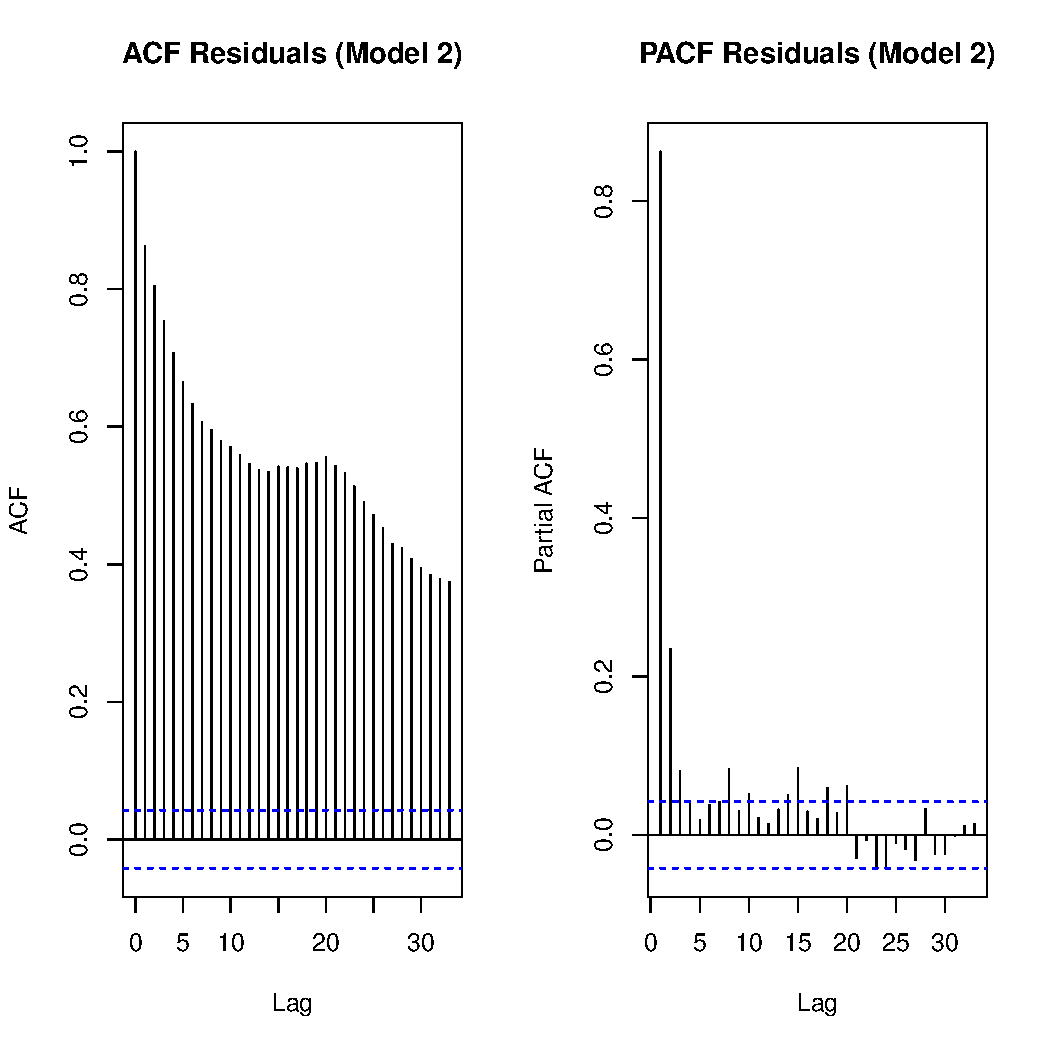
\includegraphics{FinalProject_files/figure-latex/model2-diagnostics-4.pdf}
\caption{Regression Diagnostic Plots for Log Transformed Model}
\end{figure}

\begin{Shaded}
\begin{Highlighting}[]
\NormalTok{    ljung\_box\_10\_m2 }\OtherTok{\textless{}{-}} \FunctionTok{Box.test}\NormalTok{(}\FunctionTok{residuals}\NormalTok{(model2\_log), }\AttributeTok{lag=}\DecValTok{10}\NormalTok{, }\AttributeTok{type=}\StringTok{"Ljung{-}Box"}\NormalTok{)}
\NormalTok{    ljung\_box\_20\_m2 }\OtherTok{\textless{}{-}} \FunctionTok{Box.test}\NormalTok{(}\FunctionTok{residuals}\NormalTok{(model2\_log), }\AttributeTok{lag=}\DecValTok{20}\NormalTok{, }\AttributeTok{type=}\StringTok{"Ljung{-}Box"}\NormalTok{)}
      
\NormalTok{    vif\_m2 }\OtherTok{\textless{}{-}} \FunctionTok{vif}\NormalTok{(model2\_log)}
      
\NormalTok{    cooksd\_m2 }\OtherTok{\textless{}{-}} \FunctionTok{cooks.distance}\NormalTok{(model2\_log)}
    \FunctionTok{plot}\NormalTok{(cooksd\_m2, }\AttributeTok{type=}\StringTok{"h"}\NormalTok{, }\AttributeTok{pch=}\StringTok{"*"}\NormalTok{, }\AttributeTok{cex=}\DecValTok{1}\NormalTok{, }\AttributeTok{main=}\StringTok{"Cook\textquotesingle{}s Distance Plot (Model 2)"}\NormalTok{, }\AttributeTok{ylab=}\StringTok{"Cook\textquotesingle{}s Distance"}\NormalTok{, }\AttributeTok{las=}\DecValTok{1}\NormalTok{)}
    \FunctionTok{abline}\NormalTok{(}\AttributeTok{h =} \DecValTok{4}\SpecialCharTok{/}\FunctionTok{nobs}\NormalTok{(model2\_log), }\AttributeTok{col=}\StringTok{"red"}\NormalTok{, }\AttributeTok{lty=}\DecValTok{2}\NormalTok{) }
\end{Highlighting}
\end{Shaded}

\begin{figure}
\centering
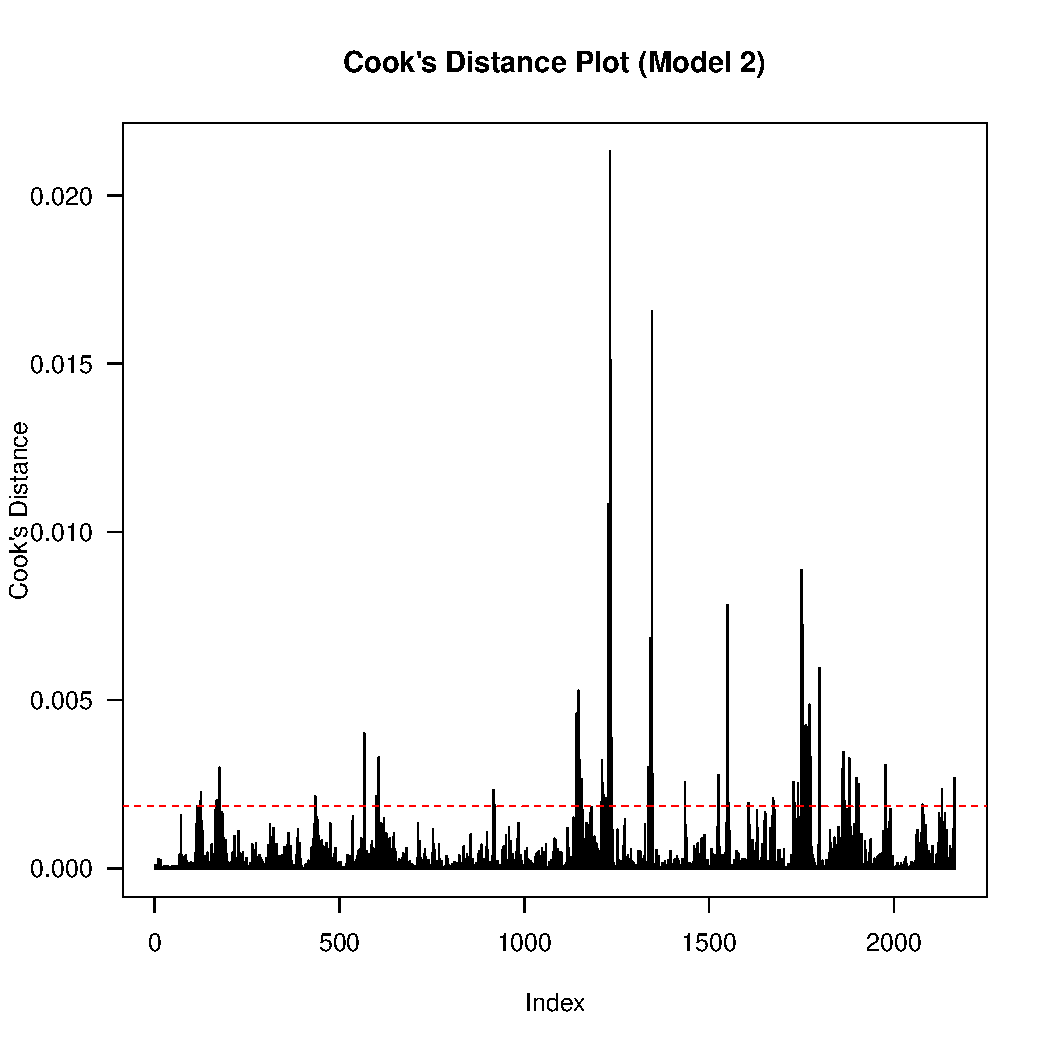
\includegraphics{FinalProject_files/figure-latex/model2-diagnostics-5.pdf}
\caption{Regression Diagnostic Plots for Log Transformed Model}
\end{figure}

\begin{Shaded}
\begin{Highlighting}[]
\NormalTok{    influential\_threshold\_4\_n\_m2 }\OtherTok{\textless{}{-}} \DecValTok{4}\SpecialCharTok{/}\FunctionTok{nobs}\NormalTok{(model2\_log)}
\NormalTok{    influential\_points\_4\_n\_m2 }\OtherTok{\textless{}{-}} \FunctionTok{which}\NormalTok{(cooksd\_m2 }\SpecialCharTok{\textgreater{}}\NormalTok{ influential\_threshold\_4\_n\_m2)}
      
    \ControlFlowTok{if}\NormalTok{ (}\SpecialCharTok{!}\FunctionTok{is.null}\NormalTok{(model2\_log}\SpecialCharTok{$}\NormalTok{na.action) }\SpecialCharTok{\&\&} \FunctionTok{length}\NormalTok{(model2\_log}\SpecialCharTok{$}\NormalTok{na.action) }\SpecialCharTok{\textgreater{}} \DecValTok{0} \SpecialCharTok{\&\&} \FunctionTok{length}\NormalTok{(final\_model\_data\_log}\SpecialCharTok{$}\NormalTok{Date[}\SpecialCharTok{{-}}\FunctionTok{na.action}\NormalTok{(model2\_log)]) }\SpecialCharTok{==} \FunctionTok{length}\NormalTok{(}\FunctionTok{residuals}\NormalTok{(model2\_log)) ) \{}
\NormalTok{      residuals\_df\_m2 }\OtherTok{\textless{}{-}} \FunctionTok{data.frame}\NormalTok{(}\AttributeTok{Date =}\NormalTok{ final\_model\_data\_log}\SpecialCharTok{$}\NormalTok{Date[}\SpecialCharTok{{-}}\NormalTok{model2\_log}\SpecialCharTok{$}\NormalTok{na.action], }\AttributeTok{Residuals =} \FunctionTok{residuals}\NormalTok{(model2\_log))}
\NormalTok{    \} }\ControlFlowTok{else} \ControlFlowTok{if}\NormalTok{ (}\FunctionTok{nrow}\NormalTok{(final\_model\_data\_log) }\SpecialCharTok{==} \FunctionTok{length}\NormalTok{(}\FunctionTok{residuals}\NormalTok{(model2\_log))) \{ }
\NormalTok{       residuals\_df\_m2 }\OtherTok{\textless{}{-}} \FunctionTok{data.frame}\NormalTok{(}\AttributeTok{Date =}\NormalTok{ final\_model\_data\_log}\SpecialCharTok{$}\NormalTok{Date, }\AttributeTok{Residuals =} \FunctionTok{residuals}\NormalTok{(model2\_log))}
\NormalTok{    \} }\ControlFlowTok{else}\NormalTok{ \{}
\NormalTok{      residuals\_df\_m2 }\OtherTok{\textless{}{-}} \ConstantTok{NULL} 
\NormalTok{    \}}
    \ControlFlowTok{if}\NormalTok{(}\SpecialCharTok{!}\FunctionTok{is.null}\NormalTok{(residuals\_df\_m2))\{}
\NormalTok{      p\_res\_time\_m2 }\OtherTok{\textless{}{-}} \FunctionTok{ggplot}\NormalTok{(residuals\_df\_m2, }\FunctionTok{aes}\NormalTok{(}\AttributeTok{x =}\NormalTok{ Date, }\AttributeTok{y =}\NormalTok{ Residuals)) }\SpecialCharTok{+}
        \FunctionTok{geom\_line}\NormalTok{(}\AttributeTok{color =} \StringTok{"coral"}\NormalTok{) }\SpecialCharTok{+} \FunctionTok{geom\_hline}\NormalTok{(}\AttributeTok{yintercept =} \DecValTok{0}\NormalTok{, }\AttributeTok{linetype =} \StringTok{"dashed"}\NormalTok{, }\AttributeTok{color =} \StringTok{"red"}\NormalTok{) }\SpecialCharTok{+}
        \FunctionTok{labs}\NormalTok{(}\AttributeTok{title =} \StringTok{"Model 2 (Log) Residuals vs. Time"}\NormalTok{, }\AttributeTok{x =} \StringTok{"Date"}\NormalTok{, }\AttributeTok{y =} \StringTok{"Residuals"}\NormalTok{) }\SpecialCharTok{+} \FunctionTok{theme\_minimal}\NormalTok{()}
      \FunctionTok{print}\NormalTok{(p\_res\_time\_m2)}
\NormalTok{    \}}
\end{Highlighting}
\end{Shaded}

\begin{figure}
\centering
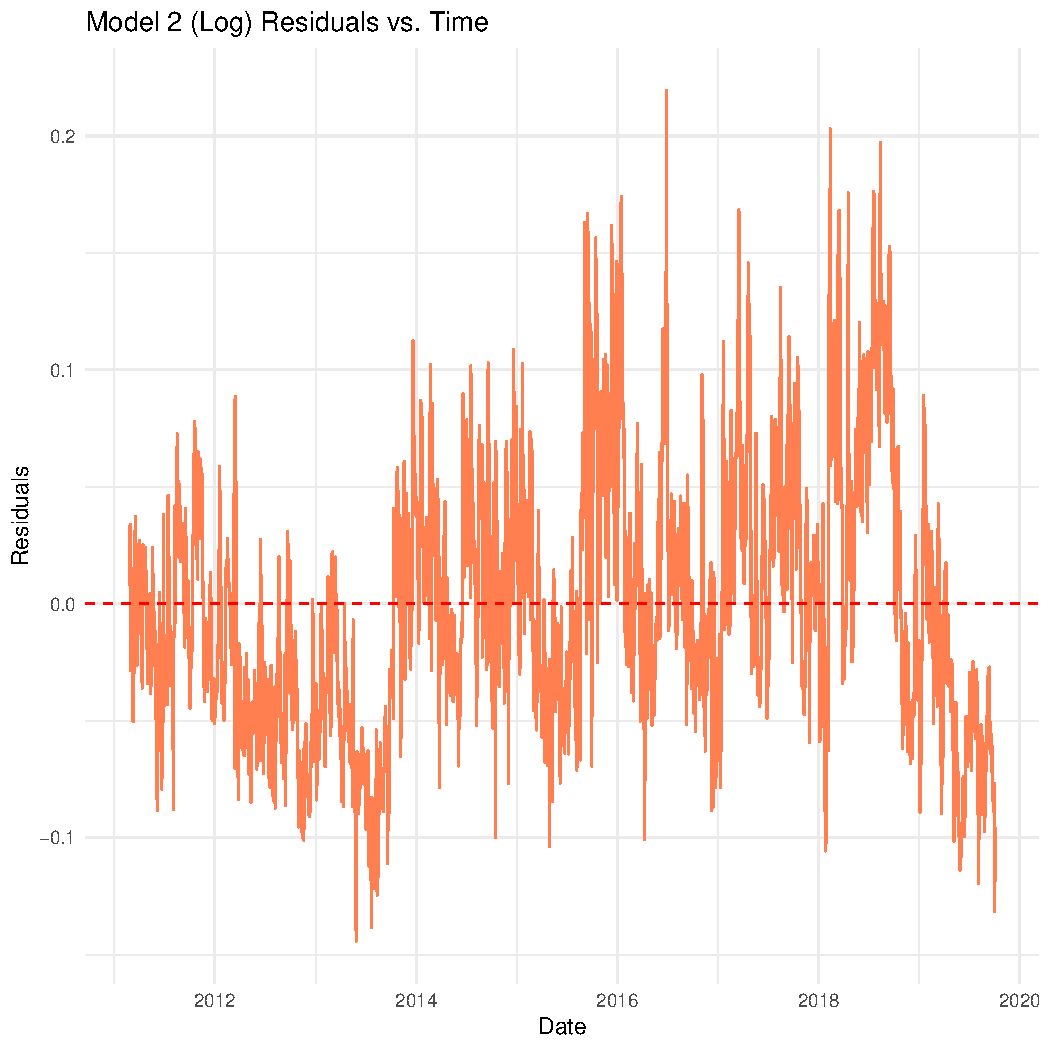
\includegraphics{FinalProject_files/figure-latex/model2-diagnostics-6.pdf}
\caption{Regression Diagnostic Plots for Log Transformed Model}
\end{figure}

\begin{Shaded}
\begin{Highlighting}[]
    \FunctionTok{cat}\NormalTok{(}\StringTok{"}\SpecialCharTok{\textbackslash{}n}\StringTok{{-}{-}{-} Shapiro{-}Wilk Normality Test (Model 2) {-}{-}{-}}\SpecialCharTok{\textbackslash{}n}\StringTok{"}\NormalTok{)}
\end{Highlighting}
\end{Shaded}

\begin{verbatim}
## 
## --- Shapiro-Wilk Normality Test (Model 2) ---
\end{verbatim}

\begin{Shaded}
\begin{Highlighting}[]
    \FunctionTok{print}\NormalTok{(shapiro\_test\_m2)}
\end{Highlighting}
\end{Shaded}

\begin{verbatim}
## 
##  Shapiro-Wilk normality test
## 
## data:  residuals(model2_log)
## W = 0.9798, p-value < 2.2e-16
\end{verbatim}

\begin{Shaded}
\begin{Highlighting}[]
    \FunctionTok{cat}\NormalTok{(}\StringTok{"}\SpecialCharTok{\textbackslash{}n}\StringTok{Skewness (Model 2 Residuals):"}\NormalTok{, }\FunctionTok{round}\NormalTok{(skewness\_m2\_res,}\DecValTok{3}\NormalTok{), }\StringTok{"}\SpecialCharTok{\textbackslash{}n}\StringTok{"}\NormalTok{)}
\end{Highlighting}
\end{Shaded}

\begin{verbatim}
## 
## Skewness (Model 2 Residuals): 0.548
\end{verbatim}

\begin{Shaded}
\begin{Highlighting}[]
    \FunctionTok{cat}\NormalTok{(}\StringTok{"Excess Kurtosis (Model 2 Residuals):"}\NormalTok{, }\FunctionTok{round}\NormalTok{(kurtosis\_m2\_res,}\DecValTok{3}\NormalTok{), }\StringTok{"}\SpecialCharTok{\textbackslash{}n}\StringTok{"}\NormalTok{)}
\end{Highlighting}
\end{Shaded}

\begin{verbatim}
## Excess Kurtosis (Model 2 Residuals): 0.083
\end{verbatim}

\begin{Shaded}
\begin{Highlighting}[]
    \FunctionTok{cat}\NormalTok{(}\StringTok{"}\SpecialCharTok{\textbackslash{}n}\StringTok{{-}{-}{-} Breusch{-}Pagan Homoscedasticity Test (Model 2) {-}{-}{-}}\SpecialCharTok{\textbackslash{}n}\StringTok{"}\NormalTok{)}
\end{Highlighting}
\end{Shaded}

\begin{verbatim}
## 
## --- Breusch-Pagan Homoscedasticity Test (Model 2) ---
\end{verbatim}

\begin{Shaded}
\begin{Highlighting}[]
    \FunctionTok{print}\NormalTok{(bp\_test\_m2)}
\end{Highlighting}
\end{Shaded}

\begin{verbatim}
## 
##  Breusch-Pagan test
## 
## data:  model2_log
## BP = 35.793, df = 6, p-value = 3.024e-06
\end{verbatim}

\begin{Shaded}
\begin{Highlighting}[]
    \FunctionTok{cat}\NormalTok{(}\StringTok{"}\SpecialCharTok{\textbackslash{}n}\StringTok{{-}{-}{-} Durbin{-}Watson Autocorrelation Test (Model 2) {-}{-}{-}}\SpecialCharTok{\textbackslash{}n}\StringTok{"}\NormalTok{)}
\end{Highlighting}
\end{Shaded}

\begin{verbatim}
## 
## --- Durbin-Watson Autocorrelation Test (Model 2) ---
\end{verbatim}

\begin{Shaded}
\begin{Highlighting}[]
    \FunctionTok{print}\NormalTok{(dw\_test\_m2)}
\end{Highlighting}
\end{Shaded}

\begin{verbatim}
## 
##  Durbin-Watson test
## 
## data:  model2_log
## DW = 0.27364, p-value < 2.2e-16
## alternative hypothesis: true autocorrelation is greater than 0
\end{verbatim}

\begin{Shaded}
\begin{Highlighting}[]
    \FunctionTok{cat}\NormalTok{(}\StringTok{"}\SpecialCharTok{\textbackslash{}n}\StringTok{{-}{-}{-} Ljung{-}Box Autocorrelation Test (10 lags, Model 2) {-}{-}{-}}\SpecialCharTok{\textbackslash{}n}\StringTok{"}\NormalTok{)}
\end{Highlighting}
\end{Shaded}

\begin{verbatim}
## 
## --- Ljung-Box Autocorrelation Test (10 lags, Model 2) ---
\end{verbatim}

\begin{Shaded}
\begin{Highlighting}[]
    \FunctionTok{print}\NormalTok{(ljung\_box\_10\_m2)}
\end{Highlighting}
\end{Shaded}

\begin{verbatim}
## 
##  Box-Ljung test
## 
## data:  residuals(model2_log)
## X-squared = 10167, df = 10, p-value < 2.2e-16
\end{verbatim}

\begin{Shaded}
\begin{Highlighting}[]
    \FunctionTok{cat}\NormalTok{(}\StringTok{"}\SpecialCharTok{\textbackslash{}n}\StringTok{{-}{-}{-} Ljung{-}Box Autocorrelation Test (20 lags, Model 2) {-}{-}{-}}\SpecialCharTok{\textbackslash{}n}\StringTok{"}\NormalTok{)}
\end{Highlighting}
\end{Shaded}

\begin{verbatim}
## 
## --- Ljung-Box Autocorrelation Test (20 lags, Model 2) ---
\end{verbatim}

\begin{Shaded}
\begin{Highlighting}[]
    \FunctionTok{print}\NormalTok{(ljung\_box\_20\_m2)}
\end{Highlighting}
\end{Shaded}

\begin{verbatim}
## 
##  Box-Ljung test
## 
## data:  residuals(model2_log)
## X-squared = 16642, df = 20, p-value < 2.2e-16
\end{verbatim}

\begin{Shaded}
\begin{Highlighting}[]
    \FunctionTok{cat}\NormalTok{(}\StringTok{"}\SpecialCharTok{\textbackslash{}n}\StringTok{{-}{-}{-} Variance Inflation Factors (Model 2) {-}{-}{-}}\SpecialCharTok{\textbackslash{}n}\StringTok{"}\NormalTok{)}
\end{Highlighting}
\end{Shaded}

\begin{verbatim}
## 
## --- Variance Inflation Factors (Model 2) ---
\end{verbatim}

\begin{Shaded}
\begin{Highlighting}[]
    \FunctionTok{print}\NormalTok{(vif\_m2)}
\end{Highlighting}
\end{Shaded}

\begin{verbatim}
##                          log_VIX_lag1                  log_RealizedVol_lag1 
##                              3.222413                              2.736576 
##                     MarketReturn_lag1                    log_Sentiment_lag1 
##                              1.590752                              1.189602 
##                     log_PC_Ratio_lag1 logVIX_logSent_Interact_centered_lag1 
##                              1.118945                              1.039206
\end{verbatim}

\begin{Shaded}
\begin{Highlighting}[]
    \FunctionTok{cat}\NormalTok{(}\StringTok{"}\SpecialCharTok{\textbackslash{}n}\StringTok{{-}{-}{-} Influential Points (Model 2) {-}{-}{-}}\SpecialCharTok{\textbackslash{}n}\StringTok{"}\NormalTok{)}
\end{Highlighting}
\end{Shaded}

\begin{verbatim}
## 
## --- Influential Points (Model 2) ---
\end{verbatim}

\begin{Shaded}
\begin{Highlighting}[]
    \FunctionTok{cat}\NormalTok{(}\StringTok{"Number of points with Cook\textquotesingle{}s D \textgreater{} 4/n:"}\NormalTok{, }\FunctionTok{length}\NormalTok{(influential\_points\_4\_n\_m2), }\StringTok{"}\SpecialCharTok{\textbackslash{}n}\StringTok{"}\NormalTok{)}
\end{Highlighting}
\end{Shaded}

\begin{verbatim}
## Number of points with Cook's D > 4/n: 100
\end{verbatim}

\begin{Shaded}
\begin{Highlighting}[]
    \ControlFlowTok{if}\NormalTok{(}\FunctionTok{length}\NormalTok{(influential\_points\_4\_n\_m2) }\SpecialCharTok{\textgreater{}} \DecValTok{0} \SpecialCharTok{\&\&} \FunctionTok{length}\NormalTok{(influential\_points\_4\_n\_m2) }\SpecialCharTok{\textless{}} \DecValTok{20}\NormalTok{) \{}
        \FunctionTok{cat}\NormalTok{(}\StringTok{"Indices of points with Cook\textquotesingle{}s D \textgreater{} 4/n (first 10):"}\NormalTok{, }\FunctionTok{paste}\NormalTok{(}\FunctionTok{head}\NormalTok{(influential\_points\_4\_n\_m2, }\DecValTok{10}\NormalTok{), }\AttributeTok{collapse=}\StringTok{", "}\NormalTok{), }\StringTok{"}\SpecialCharTok{\textbackslash{}n}\StringTok{"}\NormalTok{)}
\NormalTok{    \}}
\NormalTok{    influential\_points\_1\_m2 }\OtherTok{\textless{}{-}} \FunctionTok{which}\NormalTok{(cooksd\_m2 }\SpecialCharTok{\textgreater{}} \DecValTok{1}\NormalTok{)}
    \FunctionTok{cat}\NormalTok{(}\StringTok{"Number of points with Cook\textquotesingle{}s D \textgreater{} 1:"}\NormalTok{, }\FunctionTok{length}\NormalTok{(influential\_points\_1\_m2), }\StringTok{"}\SpecialCharTok{\textbackslash{}n}\StringTok{"}\NormalTok{)}
\end{Highlighting}
\end{Shaded}

\begin{verbatim}
## Number of points with Cook's D > 1: 0
\end{verbatim}

\begin{Shaded}
\begin{Highlighting}[]
    \ControlFlowTok{if}\NormalTok{(}\FunctionTok{length}\NormalTok{(influential\_points\_1\_m2) }\SpecialCharTok{\textgreater{}} \DecValTok{0}\NormalTok{) \{}
        \FunctionTok{cat}\NormalTok{(}\StringTok{"Indices of points with Cook\textquotesingle{}s D \textgreater{} 1:"}\NormalTok{, }\FunctionTok{paste}\NormalTok{(influential\_points\_1\_m2, }\AttributeTok{collapse=}\StringTok{", "}\NormalTok{), }\StringTok{"}\SpecialCharTok{\textbackslash{}n}\StringTok{"}\NormalTok{)}
\NormalTok{    \}}
\end{Highlighting}
\end{Shaded}

\begin{Shaded}
\begin{Highlighting}[]
\NormalTok{  nw\_lag\_m2 }\OtherTok{\textless{}{-}} \FunctionTok{floor}\NormalTok{(}\DecValTok{4}\SpecialCharTok{*}\NormalTok{(}\FunctionTok{nobs}\NormalTok{(model2\_log)}\SpecialCharTok{/}\DecValTok{100}\NormalTok{)}\SpecialCharTok{\^{}}\NormalTok{(}\DecValTok{2}\SpecialCharTok{/}\DecValTok{9}\NormalTok{)) }
\NormalTok{  model2\_log\_hac\_summary }\OtherTok{\textless{}{-}} \FunctionTok{coeftest}\NormalTok{(model2\_log, }\AttributeTok{vcov. =} \FunctionTok{NeweyWest}\NormalTok{(model2\_log, }\AttributeTok{lag =}\NormalTok{ nw\_lag\_m2, }\AttributeTok{prewhite =} \ConstantTok{FALSE}\NormalTok{, }\AttributeTok{adjust =} \ConstantTok{TRUE}\NormalTok{))}
  \FunctionTok{print}\NormalTok{(model2\_log\_hac\_summary)}
\end{Highlighting}
\end{Shaded}

t test of coefficients:

\begin{verbatim}
                                    Estimate Std. Error t value  Pr(>|t|)
\end{verbatim}

(Intercept) 4.8966239 0.0672105 72.8551 \textless{} 2.2e-16
log\_VIX\_lag1 -0.0429481 0.0157489 -2.7271 0.0064419
log\_RealizedVol\_lag1 -0.0375033 0.0101894 -3.6806 0.0002384
MarketReturn\_lag1 -0.0934942 0.0941889 -0.9926 0.3210044
log\_Sentiment\_lag1 0.0199118 0.0143564 1.3870 0.1655955
log\_PC\_Ratio\_lag1 0.0195837 0.0080337 2.4377 0.0148620
logVIX\_logSent\_Interact\_centered\_lag1 -0.0436371 0.0496226 -0.8794
0.3792928

(Intercept) \emph{\textbf{ log\_VIX\_lag1 } log\_RealizedVol\_lag1 }**
MarketReturn\_lag1\\
log\_Sentiment\_lag1\\
log\_PC\_Ratio\_lag1 *\\
logVIX\_logSent\_Interact\_centered\_lag1\\
--- Signif. codes: 0 `\emph{\textbf{' 0.001 '}' 0.01 '}' 0.05 `.' 0.1 '
' 1

\begin{Shaded}
\begin{Highlighting}[]
  \FunctionTok{colnames}\NormalTok{(model2\_log\_hac\_summary) }\OtherTok{\textless{}{-}} \FunctionTok{c}\NormalTok{(}\StringTok{"Estimate"}\NormalTok{, }\StringTok{"Std. Error"}\NormalTok{, }\StringTok{"t value"}\NormalTok{, }\StringTok{"Pr(\textgreater{}|t|)"}\NormalTok{)}
      

  \FunctionTok{stargazer}\NormalTok{(model2\_log, }
          \AttributeTok{type =} \StringTok{"latex"}\NormalTok{, }
          \AttributeTok{title =} \StringTok{"Table 4: OLSLog(SKEW) Index Regression with Newey{-}West HAC SEs (Model 2)"}\NormalTok{,}
          \AttributeTok{align =} \ConstantTok{TRUE}\NormalTok{, }
          \AttributeTok{dep.var.labels =} \StringTok{"log(CBOE SKEW Index)"}\NormalTok{,}
          \AttributeTok{covariate.labels =}\NormalTok{ my\_covariate\_labels\_m2\_log,}
          \AttributeTok{ci =} \ConstantTok{TRUE}\NormalTok{, }\AttributeTok{ci.level =} \FloatTok{0.95}\NormalTok{, }\AttributeTok{single.row =} \ConstantTok{FALSE}\NormalTok{,}
          \AttributeTok{omit.stat =} \FunctionTok{c}\NormalTok{(}\StringTok{"ser"}\NormalTok{, }\StringTok{"rsq"}\NormalTok{, }\StringTok{"f"}\NormalTok{), }
          \AttributeTok{add.lines =} \FunctionTok{list}\NormalTok{(}
              \FunctionTok{c}\NormalTok{(}\StringTok{"Observations"}\NormalTok{, }\FunctionTok{formatC}\NormalTok{(}\FunctionTok{nobs}\NormalTok{(model2\_log), }\AttributeTok{format=}\StringTok{"d"}\NormalTok{, }\AttributeTok{big.mark=}\StringTok{","}\NormalTok{)),}
              \FunctionTok{c}\NormalTok{(}\StringTok{"R{-}squared"}\NormalTok{, }\FunctionTok{format}\NormalTok{(}\FunctionTok{round}\NormalTok{(}\FunctionTok{summary}\NormalTok{(model2\_log)}\SpecialCharTok{$}\NormalTok{r.squared, }\DecValTok{3}\NormalTok{), }\AttributeTok{nsmall =} \DecValTok{3}\NormalTok{)),}
              \FunctionTok{c}\NormalTok{(}\StringTok{"Adj. R{-}squared"}\NormalTok{, }\FunctionTok{format}\NormalTok{(}\FunctionTok{round}\NormalTok{(}\FunctionTok{summary}\NormalTok{(model2\_log)}\SpecialCharTok{$}\NormalTok{adj.r.squared, }\DecValTok{3}\NormalTok{), }\AttributeTok{nsmall =} \DecValTok{3}\NormalTok{)),}
              \FunctionTok{c}\NormalTok{(}\StringTok{"F{-}statistic"}\NormalTok{, }\FunctionTok{paste0}\NormalTok{(}
                  \FunctionTok{format}\NormalTok{(}\FunctionTok{round}\NormalTok{(}\FunctionTok{summary}\NormalTok{(model2\_log)}\SpecialCharTok{$}\NormalTok{fstatistic[[}\StringTok{"value"}\NormalTok{]], }\DecValTok{2}\NormalTok{), }\AttributeTok{nsmall=}\DecValTok{2}\NormalTok{),}
                  \FunctionTok{ifelse}\NormalTok{(}\FunctionTok{pf}\NormalTok{(}\FunctionTok{summary}\NormalTok{(model2\_log)}\SpecialCharTok{$}\NormalTok{fstatistic[[}\StringTok{"value"}\NormalTok{]],}
                            \FunctionTok{summary}\NormalTok{(model2\_log)}\SpecialCharTok{$}\NormalTok{fstatistic[[}\StringTok{"numdf"}\NormalTok{]], }\FunctionTok{summary}\NormalTok{(model2\_log)}\SpecialCharTok{$}\NormalTok{fstatistic[[}\StringTok{"dendf"}\NormalTok{]], }\AttributeTok{lower.tail=}\ConstantTok{FALSE}\NormalTok{) }\SpecialCharTok{\textless{}} \FloatTok{0.001}\NormalTok{, }\StringTok{"***"}\NormalTok{,}
                         \FunctionTok{ifelse}\NormalTok{(}\FunctionTok{pf}\NormalTok{(}\FunctionTok{summary}\NormalTok{(model2\_log)}\SpecialCharTok{$}\NormalTok{fstatistic[[}\StringTok{"value"}\NormalTok{]], }\FunctionTok{summary}\NormalTok{(model2\_log)}\SpecialCharTok{$}\NormalTok{fstatistic[[}\StringTok{"numdf"}\NormalTok{]], }\FunctionTok{summary}\NormalTok{(model2\_log)}\SpecialCharTok{$}\NormalTok{fstatistic[[}\StringTok{"dendf"}\NormalTok{]], }\AttributeTok{lower.tail=}\ConstantTok{FALSE}\NormalTok{) }\SpecialCharTok{\textless{}} \FloatTok{0.01}\NormalTok{, }\StringTok{"**"}\NormalTok{,}
                                \FunctionTok{ifelse}\NormalTok{(}\FunctionTok{pf}\NormalTok{(}\FunctionTok{summary}\NormalTok{(model2\_log)}\SpecialCharTok{$}\NormalTok{fstatistic[[}\StringTok{"value"}\NormalTok{]], }\FunctionTok{summary}\NormalTok{(model2\_log)}\SpecialCharTok{$}\NormalTok{fstatistic[[}\StringTok{"numdf"}\NormalTok{]], }\FunctionTok{summary}\NormalTok{(model2\_log)}\SpecialCharTok{$}\NormalTok{fstatistic[[}\StringTok{"dendf"}\NormalTok{]], }\AttributeTok{lower.tail=}\ConstantTok{FALSE}\NormalTok{) }\SpecialCharTok{\textless{}} \FloatTok{0.05}\NormalTok{, }\StringTok{"*"}\NormalTok{, }\StringTok{""}\NormalTok{))),}
                  \StringTok{" (df = "}\NormalTok{, }\FunctionTok{summary}\NormalTok{(model2\_log)}\SpecialCharTok{$}\NormalTok{fstatistic[[}\StringTok{"numdf"}\NormalTok{]], }\StringTok{", "}\NormalTok{, }\FunctionTok{summary}\NormalTok{(model2\_log)}\SpecialCharTok{$}\NormalTok{fstatistic[[}\StringTok{"dendf"}\NormalTok{]], }\StringTok{")"}\NormalTok{))}
\NormalTok{          ),}
          \AttributeTok{star.cutoffs =} \FunctionTok{c}\NormalTok{(}\FloatTok{0.05}\NormalTok{, }\FloatTok{0.01}\NormalTok{, }\FloatTok{0.001}\NormalTok{),}
          \AttributeTok{notes =} \FunctionTok{c}\NormalTok{(}\StringTok{"$\^{}\{*\}$p$\textless{}$.05; $\^{}\{**\}$p$\textless{}$.01; $\^{}\{***\}$p$\textless{}$.001. Newey{-}West HAC Standard Errors."}\NormalTok{),}
          \AttributeTok{notes.align =} \StringTok{"l"}\NormalTok{, }
          \AttributeTok{notes.append =} \ConstantTok{FALSE}\NormalTok{, }
          \AttributeTok{header =} \ConstantTok{FALSE}\NormalTok{, }
          \AttributeTok{float =} \ConstantTok{FALSE}\NormalTok{,}
          \AttributeTok{no.space =} \ConstantTok{TRUE}\NormalTok{, }
          \AttributeTok{font.size =} \StringTok{"small"}\NormalTok{, }
          \AttributeTok{digits =} \DecValTok{3}\NormalTok{)}
\end{Highlighting}
\end{Shaded}

\begingroup 
\small 
\begin{tabular}{@{\extracolsep{5pt}}lD{.}{.}{-3} } 
\\[-1.8ex]\hline 
\hline \\[-1.8ex] 
 & \multicolumn{1}{c}{\textit{Dependent variable:}} \\ 
\cline{2-2} 
\\[-1.8ex] & \multicolumn{1}{c}{log(CBOE SKEW Index)} \\ 
\hline \\[-1.8ex] 
 log(VIX (t-1)) & -0.043^{***} \\ 
  & \multicolumn{1}{c}{(-0.058$, $-0.028)} \\ 
  log(RealizedVol (t-1)) & -0.038^{***} \\ 
  & \multicolumn{1}{c}{(-0.046$, $-0.029)} \\ 
  Market Return (t-1) & -0.093^{*} \\ 
  & \multicolumn{1}{c}{(-0.181$, $-0.006)} \\ 
  log(Sentiment (t-1)) & 0.020^{**} \\ 
  & \multicolumn{1}{c}{(0.008$, $0.032)} \\ 
  log(P/C Ratio (t-1)) & 0.020^{***} \\ 
  & \multicolumn{1}{c}{(0.008$, $0.031)} \\ 
  $\log(\text{VIX}_c\ (t{-}1)) \times \log(\text{Sent}_c\ (t{-}1))$ & -0.044^{*} \\ 
  & \multicolumn{1}{c}{(-0.086$, $-0.002)} \\ 
  Constant & 4.897^{***} \\ 
  & \multicolumn{1}{c}{(4.837$, $4.957)} \\ 
 \hline \\[-1.8ex] 
Observations & 2,165 \\ 
R-squared & 0.179 \\ 
Adj. R-squared & 0.177 \\ 
F-statistic & 78.51*** (df = 6, 2158) \\ 
Observations & \multicolumn{1}{c}{2,165} \\ 
Adjusted R$^{2}$ & \multicolumn{1}{c}{0.177} \\ 
\hline 
\hline \\[-1.8ex] 
\textit{Note:}  & \multicolumn{1}{l}{$^{*}$p$<$.05; $^{**}$p$<$.01; $^{***}$p$<$.001. Newey-West HAC Standard Errors.} \\ 
\end{tabular} 
\endgroup

\begin{Shaded}
\begin{Highlighting}[]
\NormalTok{  model3\_log }\OtherTok{\textless{}{-}} \FunctionTok{lm}\NormalTok{(log\_SKEW }\SpecialCharTok{\textasciitilde{}}\NormalTok{ log\_VIX\_lag1 }\SpecialCharTok{+}\NormalTok{ log\_RealizedVol\_lag1 }\SpecialCharTok{+}\NormalTok{ log\_PC\_Ratio\_lag1,}
                     \AttributeTok{data =}\NormalTok{ final\_model\_data\_log)}
  
  \FunctionTok{summary}\NormalTok{(model3\_log)}
\end{Highlighting}
\end{Shaded}

\begin{verbatim}
## 
## Call:
## lm(formula = log_SKEW ~ log_VIX_lag1 + log_RealizedVol_lag1 + 
##     log_PC_Ratio_lag1, data = final_model_data_log)
## 
## Residuals:
##       Min        1Q    Median        3Q       Max 
## -0.138506 -0.041790 -0.006619  0.037302  0.220947 
## 
## Coefficients:
##                       Estimate Std. Error t value Pr(>|t|)    
## (Intercept)           4.852184   0.028124 172.526  < 2e-16 ***
## log_VIX_lag1         -0.036167   0.007364  -4.911 9.73e-07 ***
## log_RealizedVol_lag1 -0.039505   0.004373  -9.033  < 2e-16 ***
## log_PC_Ratio_lag1     0.019308   0.005683   3.398 0.000692 ***
## ---
## Signif. codes:  0 '***' 0.001 '**' 0.01 '*' 0.05 '.' 0.1 ' ' 1
## 
## Residual standard error: 0.05721 on 2161 degrees of freedom
## Multiple R-squared:  0.1729, Adjusted R-squared:  0.1718 
## F-statistic: 150.6 on 3 and 2161 DF,  p-value: < 2.2e-16
\end{verbatim}

\begin{Shaded}
\begin{Highlighting}[]
  \FunctionTok{par}\NormalTok{(}\AttributeTok{mfrow=}\FunctionTok{c}\NormalTok{(}\DecValTok{2}\NormalTok{,}\DecValTok{2}\NormalTok{)); }\FunctionTok{plot}\NormalTok{(model3\_log); }\FunctionTok{par}\NormalTok{(}\AttributeTok{mfrow=}\FunctionTok{c}\NormalTok{(}\DecValTok{1}\NormalTok{,}\DecValTok{1}\NormalTok{))}
\end{Highlighting}
\end{Shaded}

\begin{figure}
\centering
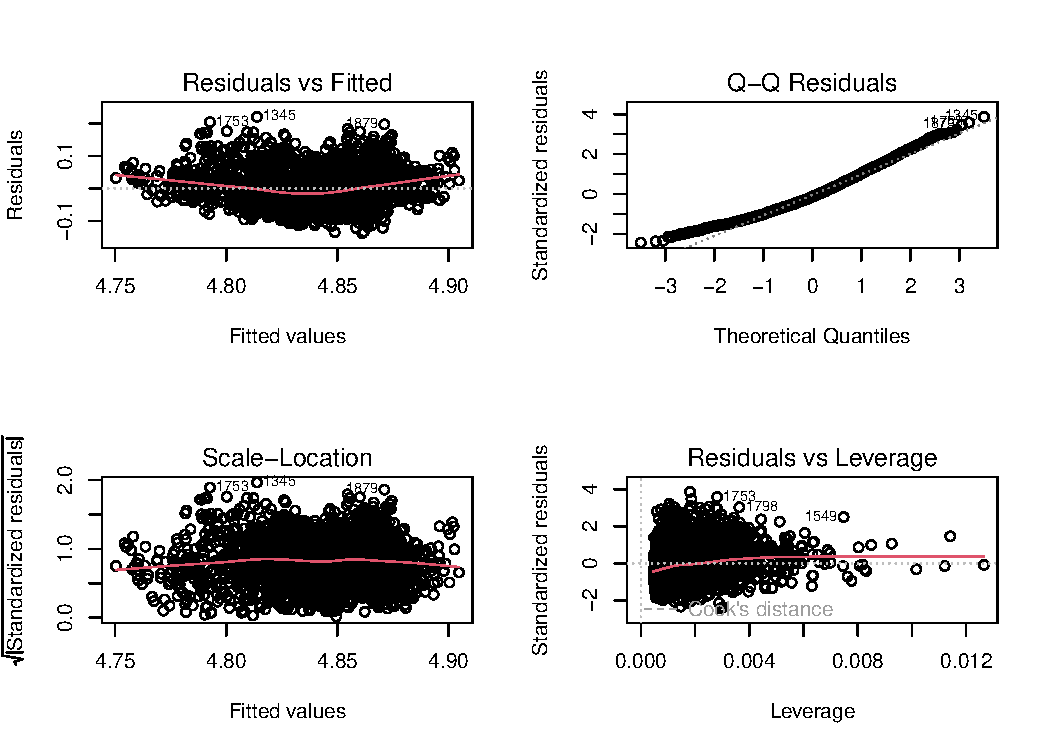
\includegraphics{FinalProject_files/figure-latex/model3-parsimonious-log-log-1.pdf}
\caption{Standard Diagnostic Plots for Model 3 (OLS)}
\end{figure}

\begin{Shaded}
\begin{Highlighting}[]
  \FunctionTok{crPlots}\NormalTok{(model3\_log, }\AttributeTok{terms =} \SpecialCharTok{\textasciitilde{}}\NormalTok{ ., }\AttributeTok{layout=}\ConstantTok{NULL}\NormalTok{, }\AttributeTok{ask=}\ConstantTok{FALSE}\NormalTok{, }\AttributeTok{smooth=}\FunctionTok{list}\NormalTok{(}\AttributeTok{smoother=}\NormalTok{loessLine, }\AttributeTok{col.lines=}\StringTok{"purple"}\NormalTok{, }\AttributeTok{spread=}\ConstantTok{FALSE}\NormalTok{), }\AttributeTok{col=}\StringTok{"darkgrey"}\NormalTok{, }\AttributeTok{pch=}\DecValTok{1}\NormalTok{, }\AttributeTok{cex=}\FloatTok{0.7}\NormalTok{, }\AttributeTok{main=}\StringTok{"Component+Residual Plots (Model 3 OLS)"}\NormalTok{)}
\end{Highlighting}
\end{Shaded}

\begin{figure}
\centering
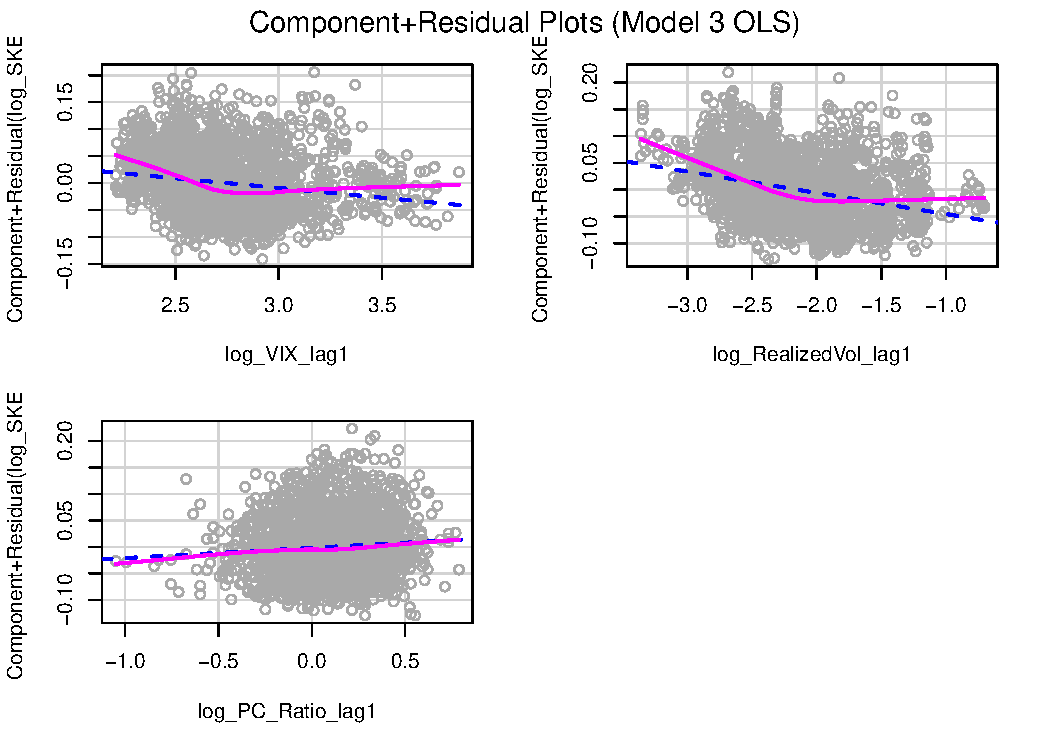
\includegraphics{FinalProject_files/figure-latex/model3-parsimonious-log-log-2.pdf}
\caption{Standard Diagnostic Plots for Model 3 (OLS)}
\end{figure}

\begin{Shaded}
\begin{Highlighting}[]
  \FunctionTok{cat}\NormalTok{(}\StringTok{"}\SpecialCharTok{\textbackslash{}n}\StringTok{{-}{-} Normality of Residuals {-}{-}}\SpecialCharTok{\textbackslash{}n}\StringTok{"}\NormalTok{)}
\end{Highlighting}
\end{Shaded}

\begin{verbatim}
## 
## -- Normality of Residuals --
\end{verbatim}

\begin{Shaded}
\begin{Highlighting}[]
  \FunctionTok{hist}\NormalTok{(}\FunctionTok{residuals}\NormalTok{(model3\_log), }\AttributeTok{breaks=}\DecValTok{50}\NormalTok{, }\AttributeTok{main=}\StringTok{"Histogram of Residuals (Model 3 OLS)"}\NormalTok{, }\AttributeTok{col=}\StringTok{"salmon"}\NormalTok{)}
\end{Highlighting}
\end{Shaded}

\begin{figure}
\centering
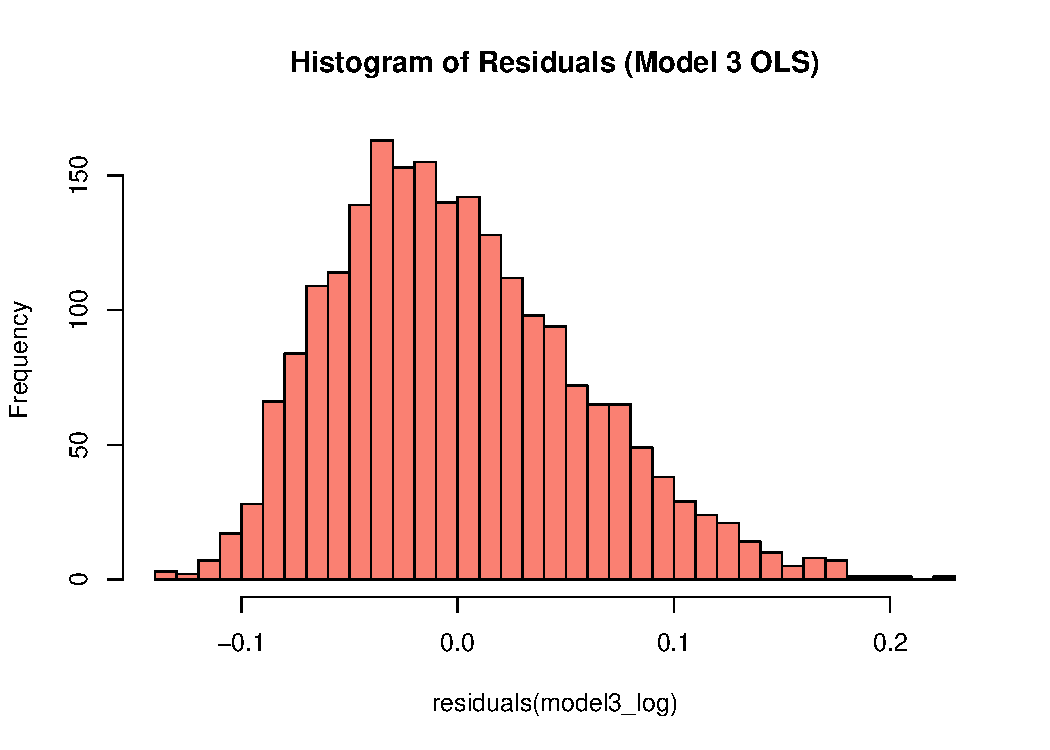
\includegraphics{FinalProject_files/figure-latex/model3-parsimonious-log-log-3.pdf}
\caption{Standard Diagnostic Plots for Model 3 (OLS)}
\end{figure}

\begin{Shaded}
\begin{Highlighting}[]
\NormalTok{  shapiro\_test\_m3 }\OtherTok{\textless{}{-}} \FunctionTok{shapiro.test}\NormalTok{(}\FunctionTok{residuals}\NormalTok{(model3\_log))}
  \FunctionTok{print}\NormalTok{(shapiro\_test\_m3)}
\end{Highlighting}
\end{Shaded}

\begin{verbatim}
## 
##  Shapiro-Wilk normality test
## 
## data:  residuals(model3_log)
## W = 0.97888, p-value < 2.2e-16
\end{verbatim}

\begin{Shaded}
\begin{Highlighting}[]
  \FunctionTok{cat}\NormalTok{(}\StringTok{"Skewness (Model 3 OLS Residuals):"}\NormalTok{, }\FunctionTok{skewness}\NormalTok{(}\FunctionTok{residuals}\NormalTok{(model3\_log)), }\StringTok{"}\SpecialCharTok{\textbackslash{}n}\StringTok{"}\NormalTok{)}
\end{Highlighting}
\end{Shaded}

\begin{verbatim}
## Skewness (Model 3 OLS Residuals): 0.5525604
\end{verbatim}

\begin{Shaded}
\begin{Highlighting}[]
  \FunctionTok{cat}\NormalTok{(}\StringTok{"Excess Kurtosis (Model 3 OLS Residuals):"}\NormalTok{, }\FunctionTok{kurtosis}\NormalTok{(}\FunctionTok{residuals}\NormalTok{(model3\_log)) }\SpecialCharTok{{-}} \DecValTok{3}\NormalTok{, }\StringTok{"}\SpecialCharTok{\textbackslash{}n}\StringTok{"}\NormalTok{)}
\end{Highlighting}
\end{Shaded}

\begin{verbatim}
## Excess Kurtosis (Model 3 OLS Residuals): 0.0569077
\end{verbatim}

\begin{Shaded}
\begin{Highlighting}[]
  \FunctionTok{cat}\NormalTok{(}\StringTok{"}\SpecialCharTok{\textbackslash{}n}\StringTok{{-}{-} Homoscedasticity (Breusch{-}Pagan Test) {-}{-}}\SpecialCharTok{\textbackslash{}n}\StringTok{"}\NormalTok{)}
\end{Highlighting}
\end{Shaded}

\begin{verbatim}
## 
## -- Homoscedasticity (Breusch-Pagan Test) --
\end{verbatim}

\begin{Shaded}
\begin{Highlighting}[]
\NormalTok{  bp\_test\_m3 }\OtherTok{\textless{}{-}} \FunctionTok{bptest}\NormalTok{(model3\_log, }\AttributeTok{studentize=}\ConstantTok{FALSE}\NormalTok{)}
  \FunctionTok{print}\NormalTok{(bp\_test\_m3)}
\end{Highlighting}
\end{Shaded}

\begin{verbatim}
## 
##  Breusch-Pagan test
## 
## data:  model3_log
## BP = 6.7456, df = 3, p-value = 0.08046
\end{verbatim}

\begin{Shaded}
\begin{Highlighting}[]
  \FunctionTok{cat}\NormalTok{(}\StringTok{"}\SpecialCharTok{\textbackslash{}n}\StringTok{{-}{-} Independence of Residuals (Durbin{-}Watson \& Ljung{-}Box) {-}{-}}\SpecialCharTok{\textbackslash{}n}\StringTok{"}\NormalTok{)}
\end{Highlighting}
\end{Shaded}

\begin{verbatim}
## 
## -- Independence of Residuals (Durbin-Watson & Ljung-Box) --
\end{verbatim}

\begin{Shaded}
\begin{Highlighting}[]
\NormalTok{  dw\_test\_m3 }\OtherTok{\textless{}{-}} \FunctionTok{dwtest}\NormalTok{(model3\_log)}
  \FunctionTok{print}\NormalTok{(dw\_test\_m3)}
\end{Highlighting}
\end{Shaded}

\begin{verbatim}
## 
##  Durbin-Watson test
## 
## data:  model3_log
## DW = 0.27002, p-value < 2.2e-16
## alternative hypothesis: true autocorrelation is greater than 0
\end{verbatim}

\begin{Shaded}
\begin{Highlighting}[]
  \FunctionTok{par}\NormalTok{(}\AttributeTok{mfrow=}\FunctionTok{c}\NormalTok{(}\DecValTok{1}\NormalTok{,}\DecValTok{2}\NormalTok{)); }\FunctionTok{acf}\NormalTok{(}\FunctionTok{residuals}\NormalTok{(model3\_log), }\AttributeTok{main=}\StringTok{"ACF Residuals (Model 3 OLS)"}\NormalTok{); }\FunctionTok{pacf}\NormalTok{(}\FunctionTok{residuals}\NormalTok{(model3\_log), }\AttributeTok{main=}\StringTok{"PACF Residuals (Model 3 OLS)"}\NormalTok{); }\FunctionTok{par}\NormalTok{(}\AttributeTok{mfrow=}\FunctionTok{c}\NormalTok{(}\DecValTok{1}\NormalTok{,}\DecValTok{1}\NormalTok{))}
\end{Highlighting}
\end{Shaded}

\begin{figure}
\centering
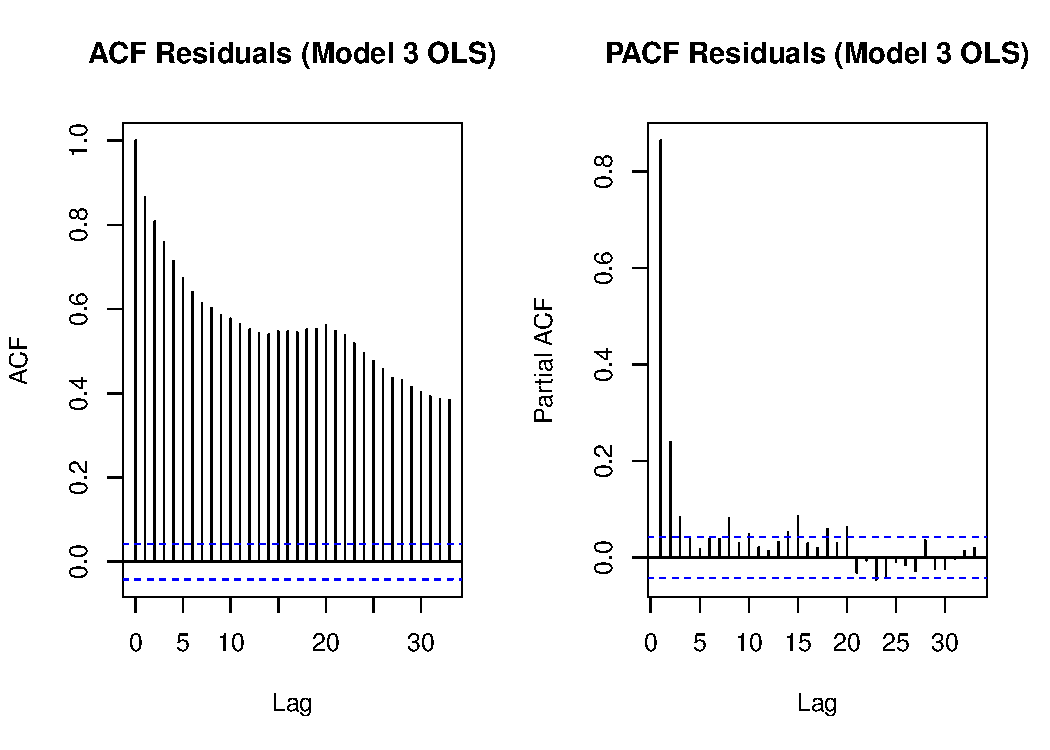
\includegraphics{FinalProject_files/figure-latex/model3-parsimonious-log-log-4.pdf}
\caption{Standard Diagnostic Plots for Model 3 (OLS)}
\end{figure}

\begin{Shaded}
\begin{Highlighting}[]
\NormalTok{  ljung\_box\_10\_m3 }\OtherTok{\textless{}{-}} \FunctionTok{Box.test}\NormalTok{(}\FunctionTok{residuals}\NormalTok{(model3\_log), }\AttributeTok{lag=}\DecValTok{10}\NormalTok{, }\AttributeTok{type=}\StringTok{"Ljung{-}Box"}\NormalTok{)}
  \FunctionTok{print}\NormalTok{(ljung\_box\_10\_m3)}
\end{Highlighting}
\end{Shaded}

\begin{verbatim}
## 
##  Box-Ljung test
## 
## data:  residuals(model3_log)
## X-squared = 10340, df = 10, p-value < 2.2e-16
\end{verbatim}

\begin{Shaded}
\begin{Highlighting}[]
  \FunctionTok{cat}\NormalTok{(}\StringTok{"}\SpecialCharTok{\textbackslash{}n}\StringTok{{-}{-} Multicollinearity (VIFs) {-}{-}}\SpecialCharTok{\textbackslash{}n}\StringTok{"}\NormalTok{)}
\end{Highlighting}
\end{Shaded}

\begin{verbatim}
## 
## -- Multicollinearity (VIFs) --
\end{verbatim}

\begin{Shaded}
\begin{Highlighting}[]
\NormalTok{  vif\_m3 }\OtherTok{\textless{}{-}} \FunctionTok{vif}\NormalTok{(model3\_log)}
  \FunctionTok{print}\NormalTok{(vif\_m3)}
\end{Highlighting}
\end{Shaded}

\begin{verbatim}
##         log_VIX_lag1 log_RealizedVol_lag1    log_PC_Ratio_lag1 
##             2.843912             2.693415             1.118418
\end{verbatim}

\begin{Shaded}
\begin{Highlighting}[]
  \FunctionTok{cat}\NormalTok{(}\StringTok{"}\SpecialCharTok{\textbackslash{}n}\StringTok{{-}{-} Influential Points (Cook\textquotesingle{}s Distance) {-}{-}}\SpecialCharTok{\textbackslash{}n}\StringTok{"}\NormalTok{)}
\end{Highlighting}
\end{Shaded}

\begin{verbatim}
## 
## -- Influential Points (Cook's Distance) --
\end{verbatim}

\begin{Shaded}
\begin{Highlighting}[]
\NormalTok{  cooksd\_m3 }\OtherTok{\textless{}{-}} \FunctionTok{cooks.distance}\NormalTok{(model3\_log)}
  \FunctionTok{plot}\NormalTok{(cooksd\_m3, }\AttributeTok{type=}\StringTok{"h"}\NormalTok{, }\AttributeTok{main=}\StringTok{"Cook\textquotesingle{}s Distance Plot (Model 3 OLS)"}\NormalTok{, }\AttributeTok{ylab=}\StringTok{"Cook\textquotesingle{}s Distance"}\NormalTok{)}
  \FunctionTok{abline}\NormalTok{(}\AttributeTok{h =} \DecValTok{4}\SpecialCharTok{/}\FunctionTok{nobs}\NormalTok{(model3\_log), }\AttributeTok{col=}\StringTok{"darkred"}\NormalTok{, }\AttributeTok{lty=}\DecValTok{2}\NormalTok{)}
\end{Highlighting}
\end{Shaded}

\begin{figure}
\centering
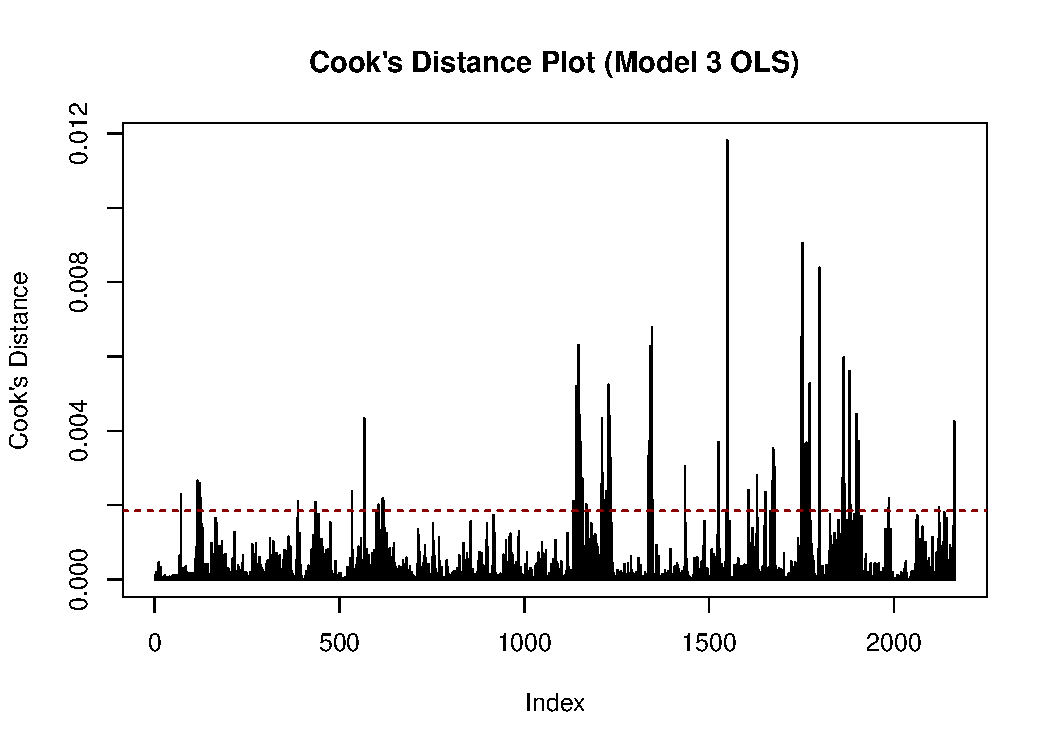
\includegraphics{FinalProject_files/figure-latex/model3-parsimonious-log-log-5.pdf}
\caption{Standard Diagnostic Plots for Model 3 (OLS)}
\end{figure}

\begin{Shaded}
\begin{Highlighting}[]
  \FunctionTok{cat}\NormalTok{(}\StringTok{"}\SpecialCharTok{\textbackslash{}n}\StringTok{{-}{-}{-} Model 3 with HAC Standard Errors {-}{-}{-}}\SpecialCharTok{\textbackslash{}n}\StringTok{"}\NormalTok{)}
\end{Highlighting}
\end{Shaded}

\begin{verbatim}
## 
## --- Model 3 with HAC Standard Errors ---
\end{verbatim}

\begin{Shaded}
\begin{Highlighting}[]
\NormalTok{  nw\_lag\_m3 }\OtherTok{\textless{}{-}} \FunctionTok{floor}\NormalTok{(}\DecValTok{4}\SpecialCharTok{*}\NormalTok{(}\FunctionTok{nobs}\NormalTok{(model3\_log)}\SpecialCharTok{/}\DecValTok{100}\NormalTok{)}\SpecialCharTok{\^{}}\NormalTok{(}\DecValTok{2}\SpecialCharTok{/}\DecValTok{9}\NormalTok{))}
\NormalTok{  model3\_log\_hac\_summary }\OtherTok{\textless{}{-}} \FunctionTok{coeftest}\NormalTok{(model3\_log, }\AttributeTok{vcov. =} \FunctionTok{NeweyWest}\NormalTok{(model3\_log, }\AttributeTok{lag =}\NormalTok{ nw\_lag\_m3, }\AttributeTok{prewhite =} \ConstantTok{FALSE}\NormalTok{, }\AttributeTok{adjust =} \ConstantTok{TRUE}\NormalTok{))}
  \FunctionTok{print}\NormalTok{(model3\_log\_hac\_summary)}
\end{Highlighting}
\end{Shaded}

\begin{verbatim}
## 
## t test of coefficients:
## 
##                        Estimate Std. Error t value  Pr(>|t|)    
## (Intercept)           4.8521842  0.0591626 82.0144 < 2.2e-16 ***
## log_VIX_lag1         -0.0361670  0.0148889 -2.4291   0.01522 *  
## log_RealizedVol_lag1 -0.0395053  0.0101164 -3.9051 9.709e-05 ***
## log_PC_Ratio_lag1     0.0193084  0.0080644  2.3943   0.01674 *  
## ---
## Signif. codes:  0 '***' 0.001 '**' 0.01 '*' 0.05 '.' 0.1 ' ' 1
\end{verbatim}

\begin{Shaded}
\begin{Highlighting}[]
  \FunctionTok{cat}\NormalTok{(}\StringTok{"}\SpecialCharTok{\textbackslash{}n}\StringTok{{-}{-}{-} Stargazer Table for Model 3 (HAC SEs) {-}{-}{-}}\SpecialCharTok{\textbackslash{}n}\StringTok{"}\NormalTok{)}
\end{Highlighting}
\end{Shaded}

\begin{verbatim}
## 
## --- Stargazer Table for Model 3 (HAC SEs) ---
\end{verbatim}

\begin{Shaded}
\begin{Highlighting}[]
\NormalTok{  my\_covariate\_labels\_m3\_log }\OtherTok{\textless{}{-}} \FunctionTok{c}\NormalTok{(}
    \StringTok{"log(VIX (t{-}1))"}\NormalTok{,}
    \StringTok{"log(RealizedVol (t{-}1))"}\NormalTok{,}
    \StringTok{"log(P/C Ratio (t{-}1))"}
\NormalTok{  )}
  
\NormalTok{  nw\_lag\_m3\_for\_table }\OtherTok{\textless{}{-}} \FunctionTok{floor}\NormalTok{(}\DecValTok{4}\SpecialCharTok{*}\NormalTok{(}\FunctionTok{nobs}\NormalTok{(model3\_log)}\SpecialCharTok{/}\DecValTok{100}\NormalTok{)}\SpecialCharTok{\^{}}\NormalTok{(}\DecValTok{2}\SpecialCharTok{/}\DecValTok{9}\NormalTok{))}
\NormalTok{  model3\_log\_hac\_summary }\OtherTok{\textless{}{-}} \FunctionTok{coeftest}\NormalTok{(model3\_log, }\AttributeTok{vcov. =} \FunctionTok{NeweyWest}\NormalTok{(model3\_log, }\AttributeTok{lag =}\NormalTok{ nw\_lag\_m3\_for\_table, }\AttributeTok{prewhite =} \ConstantTok{FALSE}\NormalTok{, }\AttributeTok{adjust =} \ConstantTok{TRUE}\NormalTok{))}
\NormalTok{  dw\_test\_m3 }\OtherTok{\textless{}{-}} \FunctionTok{dwtest}\NormalTok{(model3\_log)}


  
\NormalTok{  my\_covariate\_labels\_m3\_log }\OtherTok{\textless{}{-}} \FunctionTok{c}\NormalTok{(}
    \StringTok{"log(VIX (t{-}1))"}\NormalTok{,}
    \StringTok{"log(RealizedVol (t{-}1))"}\NormalTok{,}
    \StringTok{"log(P/C Ratio (t{-}1))"}
\NormalTok{  )}
\end{Highlighting}
\end{Shaded}

\begin{Shaded}
\begin{Highlighting}[]
\FunctionTok{stargazer}\NormalTok{(model3\_log,}
          \AttributeTok{type =} \StringTok{"latex"}\NormalTok{,}
          \AttributeTok{title =} \StringTok{"Table 5: Parsimonious Log(SKEW) Index Regression with Newey{-}West HAC SEs (Model 3)"}\NormalTok{,}
          \AttributeTok{align =} \ConstantTok{TRUE}\NormalTok{,}
          \AttributeTok{dep.var.labels =} \StringTok{"log(CBOE SKEW Index)"}\NormalTok{,}
          \AttributeTok{covariate.labels =}\NormalTok{ my\_covariate\_labels\_m3\_log,}
          \AttributeTok{coef =} \FunctionTok{list}\NormalTok{(}\FunctionTok{coef}\NormalTok{(model3\_log)),}
          \AttributeTok{se =} \FunctionTok{list}\NormalTok{(model3\_log\_hac\_summary[, }\StringTok{"Std. Error"}\NormalTok{]),}
          \AttributeTok{t =} \FunctionTok{list}\NormalTok{(model3\_log\_hac\_summary[, }\StringTok{"t value"}\NormalTok{]),}
          \AttributeTok{p =} \FunctionTok{list}\NormalTok{(model3\_log\_hac\_summary[, }\StringTok{"Pr(\textgreater{}|t|)"}\NormalTok{]),}
          \AttributeTok{ci =} \ConstantTok{TRUE}\NormalTok{, }
          \AttributeTok{omit.stat =} \FunctionTok{c}\NormalTok{(}\StringTok{"ser"}\NormalTok{, }\StringTok{"f"}\NormalTok{, }\StringTok{"bic"}\NormalTok{, }\StringTok{"aic"}\NormalTok{, }\StringTok{"ll"}\NormalTok{),}
          \AttributeTok{add.lines =} \FunctionTok{list}\NormalTok{(}
            \FunctionTok{c}\NormalTok{(}\StringTok{"Observations"}\NormalTok{, }\FunctionTok{formatC}\NormalTok{(}\FunctionTok{nobs}\NormalTok{(model3\_log), }\AttributeTok{format=}\StringTok{"d"}\NormalTok{, }\AttributeTok{big.mark=}\StringTok{","}\NormalTok{)),}
            \FunctionTok{c}\NormalTok{(}\StringTok{"R{-}squared (OLS)"}\NormalTok{, }\FunctionTok{format}\NormalTok{(}\FunctionTok{round}\NormalTok{(}\FunctionTok{summary}\NormalTok{(model3\_log)}\SpecialCharTok{$}\NormalTok{r.squared, }\DecValTok{3}\NormalTok{), }\AttributeTok{nsmall =} \DecValTok{3}\NormalTok{)),}
            \FunctionTok{c}\NormalTok{(}\StringTok{"Adj. R{-}squared (OLS)"}\NormalTok{, }\FunctionTok{format}\NormalTok{(}\FunctionTok{round}\NormalTok{(}\FunctionTok{summary}\NormalTok{(model3\_log)}\SpecialCharTok{$}\NormalTok{adj.r.squared, }\DecValTok{3}\NormalTok{), }\AttributeTok{nsmall =} \DecValTok{3}\NormalTok{)),}
            \FunctionTok{c}\NormalTok{(}\StringTok{"Newey{-}West Lag Chosen"}\NormalTok{, nw\_lag\_m3\_for\_table),}
            \FunctionTok{c}\NormalTok{(}\StringTok{"Durbin{-}Watson Stat. (OLS)"}\NormalTok{, }\FunctionTok{format}\NormalTok{(}\FunctionTok{round}\NormalTok{(dw\_test\_m3}\SpecialCharTok{$}\NormalTok{statistic, }\DecValTok{2}\NormalTok{), }\AttributeTok{nsmall=}\DecValTok{2}\NormalTok{))}
\NormalTok{          ),}
          \AttributeTok{star.cutoffs =} \FunctionTok{c}\NormalTok{(}\FloatTok{0.05}\NormalTok{, }\FloatTok{0.01}\NormalTok{, }\FloatTok{0.001}\NormalTok{),}
          \AttributeTok{notes =} \StringTok{"$\^{}\{*\}$p$\textless{}$.05; $\^{}\{**\}$p$\textless{}$.01; $\^{}\{***\}$p$\textless{}$.001. Newey{-}West HAC Standard Errors."}\NormalTok{,}
          \AttributeTok{notes.align =} \StringTok{"l"}\NormalTok{,}
          \AttributeTok{notes.append =} \ConstantTok{FALSE}\NormalTok{,}
          \AttributeTok{header =} \ConstantTok{FALSE}\NormalTok{,}
          \AttributeTok{float =} \ConstantTok{FALSE}\NormalTok{,}
          \AttributeTok{no.space =} \ConstantTok{TRUE}\NormalTok{,}
          \AttributeTok{font.size =} \StringTok{"small"}\NormalTok{,}
          \AttributeTok{digits =} \DecValTok{3}\NormalTok{)}
\end{Highlighting}
\end{Shaded}

\begingroup 
\small 
\begin{tabular}{@{\extracolsep{5pt}}lD{.}{.}{-3} } 
\\[-1.8ex]\hline 
\hline \\[-1.8ex] 
 & \multicolumn{1}{c}{\textit{Dependent variable:}} \\ 
\cline{2-2} 
\\[-1.8ex] & \multicolumn{1}{c}{log(CBOE SKEW Index)} \\ 
\hline \\[-1.8ex] 
 log(VIX (t-1)) & -0.036^{*} \\ 
  & \multicolumn{1}{c}{(-0.065$, $-0.007)} \\ 
  log(RealizedVol (t-1)) & -0.040^{***} \\ 
  & \multicolumn{1}{c}{(-0.059$, $-0.020)} \\ 
  log(P/C Ratio (t-1)) & 0.019^{*} \\ 
  & \multicolumn{1}{c}{(0.004$, $0.035)} \\ 
  Constant & 4.852^{***} \\ 
  & \multicolumn{1}{c}{(4.736$, $4.968)} \\ 
 \hline \\[-1.8ex] 
Observations & 2,165 \\ 
R-squared (OLS) & 0.173 \\ 
Adj. R-squared (OLS) & 0.172 \\ 
Newey-West Lag Chosen & 7 \\ 
Durbin-Watson Stat. (OLS) & 0.27 \\ 
Observations & \multicolumn{1}{c}{2,165} \\ 
R$^{2}$ & \multicolumn{1}{c}{0.173} \\ 
Adjusted R$^{2}$ & \multicolumn{1}{c}{0.172} \\ 
\hline 
\hline \\[-1.8ex] 
\textit{Note:}  & \multicolumn{1}{l}{$^{*}$p$<$.05; $^{**}$p$<$.01; $^{***}$p$<$.001. Newey-West HAC Standard Errors.} \\ 
\end{tabular} 
\endgroup

\begin{Shaded}
\begin{Highlighting}[]
\NormalTok{  calculate\_rmse }\OtherTok{\textless{}{-}} \ControlFlowTok{function}\NormalTok{(actual, predicted) \{}
    \FunctionTok{sqrt}\NormalTok{(}\FunctionTok{mean}\NormalTok{((actual }\SpecialCharTok{{-}}\NormalTok{ predicted)}\SpecialCharTok{\^{}}\DecValTok{2}\NormalTok{, }\AttributeTok{na.rm =} \ConstantTok{TRUE}\NormalTok{))}
\NormalTok{  \}}
  
\NormalTok{  calculate\_rsquared\_oos }\OtherTok{\textless{}{-}} \ControlFlowTok{function}\NormalTok{(actual, predicted) \{}
\NormalTok{    tss }\OtherTok{\textless{}{-}} \FunctionTok{sum}\NormalTok{((actual }\SpecialCharTok{{-}} \FunctionTok{mean}\NormalTok{(actual, }\AttributeTok{na.rm =} \ConstantTok{TRUE}\NormalTok{))}\SpecialCharTok{\^{}}\DecValTok{2}\NormalTok{, }\AttributeTok{na.rm =} \ConstantTok{TRUE}\NormalTok{)}
\NormalTok{    rss }\OtherTok{\textless{}{-}} \FunctionTok{sum}\NormalTok{((actual }\SpecialCharTok{{-}}\NormalTok{ predicted)}\SpecialCharTok{\^{}}\DecValTok{2}\NormalTok{, }\AttributeTok{na.rm =} \ConstantTok{TRUE}\NormalTok{)}
    \ControlFlowTok{if}\NormalTok{ (tss }\SpecialCharTok{==} \DecValTok{0}\NormalTok{) }\FunctionTok{return}\NormalTok{(}\ConstantTok{NA}\NormalTok{)}
    \FunctionTok{return}\NormalTok{(}\DecValTok{1} \SpecialCharTok{{-}}\NormalTok{ (rss }\SpecialCharTok{/}\NormalTok{ tss))}
\NormalTok{  \}}
  
  \FunctionTok{cat}\NormalTok{(}\StringTok{"}\SpecialCharTok{\textbackslash{}n}\StringTok{{-}{-}{-} Model 1 (Levels): Rolling Origin k{-}Fold Cross{-}Validation {-}{-}{-}}\SpecialCharTok{\textbackslash{}n}\StringTok{"}\NormalTok{)}
\end{Highlighting}
\end{Shaded}

\begin{verbatim}
## 
## --- Model 1 (Levels): Rolling Origin k-Fold Cross-Validation ---
\end{verbatim}

\begin{Shaded}
\begin{Highlighting}[]
\NormalTok{  data\_for\_cv\_m1 }\OtherTok{\textless{}{-}}\NormalTok{ final\_model\_data}
\NormalTok{  k\_folds\_m1 }\OtherTok{\textless{}{-}} \DecValTok{5}
\NormalTok{  n\_obs\_m1 }\OtherTok{\textless{}{-}} \FunctionTok{nrow}\NormalTok{(data\_for\_cv\_m1)}
\NormalTok{  initial\_train\_percent\_m1 }\OtherTok{\textless{}{-}} \FloatTok{0.70}
\NormalTok{  initial\_train\_window\_m1 }\OtherTok{\textless{}{-}} \FunctionTok{floor}\NormalTok{(initial\_train\_percent\_m1 }\SpecialCharTok{*}\NormalTok{ n\_obs\_m1)}
\NormalTok{  remaining\_obs\_m1 }\OtherTok{\textless{}{-}}\NormalTok{ n\_obs\_m1 }\SpecialCharTok{{-}}\NormalTok{ initial\_train\_window\_m1}
\NormalTok{  fold\_size\_m1 }\OtherTok{\textless{}{-}} \FunctionTok{floor}\NormalTok{(remaining\_obs\_m1 }\SpecialCharTok{/}\NormalTok{ k\_folds\_m1)}
  
\NormalTok{  rmse\_scores\_m1 }\OtherTok{\textless{}{-}} \FunctionTok{numeric}\NormalTok{(k\_folds\_m1)}
\NormalTok{  rsquared\_oos\_scores\_m1 }\OtherTok{\textless{}{-}} \FunctionTok{numeric}\NormalTok{(k\_folds\_m1)}
  
\NormalTok{  model1\_formula\_cv }\OtherTok{\textless{}{-}}\NormalTok{ SKEW }\SpecialCharTok{\textasciitilde{}}\NormalTok{ VIX\_lag1 }\SpecialCharTok{+}\NormalTok{ VIX\_sq\_lag1 }\SpecialCharTok{+}\NormalTok{ RealizedVol\_lag1 }\SpecialCharTok{+}
\NormalTok{                              MarketReturn\_lag1 }\SpecialCharTok{+}\NormalTok{ Sentiment\_lag1 }\SpecialCharTok{+}\NormalTok{ PC\_Ratio\_lag1 }\SpecialCharTok{+}
\NormalTok{                              VIX\_Sent\_Interact\_centered\_lag1}
  
  \ControlFlowTok{if}\NormalTok{ (fold\_size\_m1 }\SpecialCharTok{\textgreater{}} \DecValTok{0}\NormalTok{) \{}
    \ControlFlowTok{for}\NormalTok{ (i }\ControlFlowTok{in} \DecValTok{1}\SpecialCharTok{:}\NormalTok{k\_folds\_m1) \{}
\NormalTok{      train\_end\_idx }\OtherTok{\textless{}{-}}\NormalTok{ initial\_train\_window\_m1 }\SpecialCharTok{+}\NormalTok{ (i }\SpecialCharTok{{-}} \DecValTok{1}\NormalTok{) }\SpecialCharTok{*}\NormalTok{ fold\_size\_m1}
\NormalTok{      test\_start\_idx }\OtherTok{\textless{}{-}}\NormalTok{ train\_end\_idx }\SpecialCharTok{+} \DecValTok{1}
      \ControlFlowTok{if}\NormalTok{ (i }\SpecialCharTok{\textless{}}\NormalTok{ k\_folds\_m1) \{}
\NormalTok{        test\_end\_idx }\OtherTok{\textless{}{-}}\NormalTok{ train\_end\_idx }\SpecialCharTok{+}\NormalTok{ fold\_size\_m1}
\NormalTok{      \} }\ControlFlowTok{else}\NormalTok{ \{}
\NormalTok{        test\_end\_idx }\OtherTok{\textless{}{-}}\NormalTok{ n\_obs\_m1}
\NormalTok{      \}}
  
      \ControlFlowTok{if}\NormalTok{ (test\_start\_idx }\SpecialCharTok{\textgreater{}}\NormalTok{ n\_obs\_m1) \{}
\NormalTok{        rmse\_scores\_m1[i] }\OtherTok{\textless{}{-}} \ConstantTok{NA}
\NormalTok{        rsquared\_oos\_scores\_m1[i] }\OtherTok{\textless{}{-}} \ConstantTok{NA}
        \FunctionTok{cat}\NormalTok{(}\FunctionTok{paste}\NormalTok{(}\StringTok{"Fold"}\NormalTok{, i, }\StringTok{"(Model 1): No test data remaining. Skipping.}\SpecialCharTok{\textbackslash{}n}\StringTok{"}\NormalTok{))}
        \ControlFlowTok{next}
\NormalTok{      \}}
      
\NormalTok{      current\_train\_data\_m1 }\OtherTok{\textless{}{-}}\NormalTok{ data\_for\_cv\_m1[}\DecValTok{1}\SpecialCharTok{:}\NormalTok{train\_end\_idx, ]}
\NormalTok{      current\_test\_data\_m1  }\OtherTok{\textless{}{-}}\NormalTok{ data\_for\_cv\_m1[test\_start\_idx}\SpecialCharTok{:}\NormalTok{test\_end\_idx, ]}
  
      \ControlFlowTok{if}\NormalTok{ (}\FunctionTok{nrow}\NormalTok{(current\_test\_data\_m1) }\SpecialCharTok{==} \DecValTok{0}\NormalTok{) \{}
\NormalTok{          rmse\_scores\_m1[i] }\OtherTok{\textless{}{-}} \ConstantTok{NA}
\NormalTok{          rsquared\_oos\_scores\_m1[i] }\OtherTok{\textless{}{-}} \ConstantTok{NA}
          \FunctionTok{cat}\NormalTok{(}\FunctionTok{paste}\NormalTok{(}\StringTok{"Fold"}\NormalTok{, i, }\StringTok{"(Model 1): Test data has 0 rows. Skipping.}\SpecialCharTok{\textbackslash{}n}\StringTok{"}\NormalTok{))}
          \ControlFlowTok{next}
\NormalTok{      \}}
  
\NormalTok{      model\_fit\_cv\_m1 }\OtherTok{\textless{}{-}} \FunctionTok{lm}\NormalTok{(model1\_formula\_cv, }\AttributeTok{data =}\NormalTok{ current\_train\_data\_m1)}
\NormalTok{      predictions\_cv\_m1 }\OtherTok{\textless{}{-}} \FunctionTok{predict}\NormalTok{(model\_fit\_cv\_m1, }\AttributeTok{newdata =}\NormalTok{ current\_test\_data\_m1)}
\NormalTok{      actuals\_cv\_m1 }\OtherTok{\textless{}{-}}\NormalTok{ current\_test\_data\_m1}\SpecialCharTok{$}\NormalTok{SKEW}
      
\NormalTok{      rmse\_scores\_m1[i] }\OtherTok{\textless{}{-}} \FunctionTok{calculate\_rmse}\NormalTok{(actuals\_cv\_m1, predictions\_cv\_m1)}
\NormalTok{      rsquared\_oos\_scores\_m1[i] }\OtherTok{\textless{}{-}} \FunctionTok{calculate\_rsquared\_oos}\NormalTok{(actuals\_cv\_m1, predictions\_cv\_m1)}
      
      \FunctionTok{cat}\NormalTok{(}\FunctionTok{paste}\NormalTok{(}\StringTok{"Fold"}\NormalTok{, i, }\StringTok{"RMSE (Model 1, levels):"}\NormalTok{, }\FunctionTok{round}\NormalTok{(rmse\_scores\_m1[i], }\DecValTok{4}\NormalTok{), }
                \StringTok{"| OOS R{-}squared (Model 1, levels):"}\NormalTok{, }\FunctionTok{round}\NormalTok{(rsquared\_oos\_scores\_m1[i], }\DecValTok{4}\NormalTok{),}
                \StringTok{"| Train Size:"}\NormalTok{, }\FunctionTok{nrow}\NormalTok{(current\_train\_data\_m1), }
                \StringTok{"| Test Size:"}\NormalTok{, }\FunctionTok{nrow}\NormalTok{(current\_test\_data\_m1), }\StringTok{"}\SpecialCharTok{\textbackslash{}n}\StringTok{"}\NormalTok{))}
\NormalTok{    \}}
    
\NormalTok{    mean\_cv\_rmse\_m1 }\OtherTok{\textless{}{-}} \FunctionTok{mean}\NormalTok{(rmse\_scores\_m1, }\AttributeTok{na.rm =} \ConstantTok{TRUE}\NormalTok{)}
\NormalTok{    sd\_cv\_rmse\_m1 }\OtherTok{\textless{}{-}} \FunctionTok{sd}\NormalTok{(rmse\_scores\_m1, }\AttributeTok{na.rm =} \ConstantTok{TRUE}\NormalTok{)}
\NormalTok{    mean\_cv\_rsquared\_oos\_m1 }\OtherTok{\textless{}{-}} \FunctionTok{mean}\NormalTok{(rsquared\_oos\_scores\_m1, }\AttributeTok{na.rm =} \ConstantTok{TRUE}\NormalTok{)}
    
    \FunctionTok{cat}\NormalTok{(}\FunctionTok{paste}\NormalTok{(}\StringTok{"}\SpecialCharTok{\textbackslash{}n}\StringTok{Average Cross{-}Validated RMSE (Model 1, levels):"}\NormalTok{, }\FunctionTok{round}\NormalTok{(mean\_cv\_rmse\_m1, }\DecValTok{4}\NormalTok{), }\StringTok{"}\SpecialCharTok{\textbackslash{}n}\StringTok{"}\NormalTok{))}
    \FunctionTok{cat}\NormalTok{(}\FunctionTok{paste}\NormalTok{(}\StringTok{"Std Dev of Cross{-}Validated RMSE (Model 1, levels):"}\NormalTok{, }\FunctionTok{round}\NormalTok{(sd\_cv\_rmse\_m1, }\DecValTok{4}\NormalTok{), }\StringTok{"}\SpecialCharTok{\textbackslash{}n}\StringTok{"}\NormalTok{))}
    \FunctionTok{cat}\NormalTok{(}\FunctionTok{paste}\NormalTok{(}\StringTok{"Average Out{-}of{-}Sample R{-}squared (Model 1, levels):"}\NormalTok{, }\FunctionTok{round}\NormalTok{(mean\_cv\_rsquared\_oos\_m1, }\DecValTok{4}\NormalTok{), }\StringTok{"}\SpecialCharTok{\textbackslash{}n}\StringTok{"}\NormalTok{))}
    
\NormalTok{  \} }\ControlFlowTok{else}\NormalTok{ \{}
    \FunctionTok{cat}\NormalTok{(}\StringTok{"Fold size for Model 1 CV is 0. Increase k\_folds or adjust initial\_train\_percent\_m1.}\SpecialCharTok{\textbackslash{}n}\StringTok{"}\NormalTok{)}
\NormalTok{  \}}
\end{Highlighting}
\end{Shaded}

\begin{verbatim}
## Fold 1 RMSE (Model 1, levels): 10.4261 | OOS R-squared (Model 1, levels): -1.6195 | Train Size: 1515 | Test Size: 130 
## Fold 2 RMSE (Model 1, levels): 8.9033 | OOS R-squared (Model 1, levels): -0.8249 | Train Size: 1645 | Test Size: 130 
## Fold 3 RMSE (Model 1, levels): 13.1251 | OOS R-squared (Model 1, levels): -1.1375 | Train Size: 1775 | Test Size: 130 
## Fold 4 RMSE (Model 1, levels): 5.6604 | OOS R-squared (Model 1, levels): 0.3514 | Train Size: 1905 | Test Size: 130 
## Fold 5 RMSE (Model 1, levels): 8.903 | OOS R-squared (Model 1, levels): -2.5805 | Train Size: 2035 | Test Size: 130 
## 
## Average Cross-Validated RMSE (Model 1, levels): 9.4036 
## Std Dev of Cross-Validated RMSE (Model 1, levels): 2.7114 
## Average Out-of-Sample R-squared (Model 1, levels): -1.1622
\end{verbatim}

\begin{Shaded}
\begin{Highlighting}[]
  \FunctionTok{cat}\NormalTok{(}\StringTok{"}\SpecialCharTok{\textbackslash{}n\textbackslash{}n}\StringTok{{-}{-}{-} Model 2 (Log{-}Log): Rolling Origin k{-}Fold Cross{-}Validation {-}{-}{-}}\SpecialCharTok{\textbackslash{}n}\StringTok{"}\NormalTok{)}
\end{Highlighting}
\end{Shaded}

\begin{verbatim}
## 
## 
## --- Model 2 (Log-Log): Rolling Origin k-Fold Cross-Validation ---
\end{verbatim}

\begin{Shaded}
\begin{Highlighting}[]
\NormalTok{  data\_for\_cv\_m2 }\OtherTok{\textless{}{-}}\NormalTok{ final\_model\_data\_log}
\NormalTok{  k\_folds\_m2 }\OtherTok{\textless{}{-}} \DecValTok{5}
\NormalTok{  n\_obs\_m2 }\OtherTok{\textless{}{-}} \FunctionTok{nrow}\NormalTok{(data\_for\_cv\_m2)}
\NormalTok{  initial\_train\_percent\_m2 }\OtherTok{\textless{}{-}} \FloatTok{0.70}
\NormalTok{  initial\_train\_window\_m2 }\OtherTok{\textless{}{-}} \FunctionTok{floor}\NormalTok{(initial\_train\_percent\_m2 }\SpecialCharTok{*}\NormalTok{ n\_obs\_m2)}
\NormalTok{  remaining\_obs\_m2 }\OtherTok{\textless{}{-}}\NormalTok{ n\_obs\_m2 }\SpecialCharTok{{-}}\NormalTok{ initial\_train\_window\_m2}
\NormalTok{  fold\_size\_m2 }\OtherTok{\textless{}{-}} \FunctionTok{floor}\NormalTok{(remaining\_obs\_m2 }\SpecialCharTok{/}\NormalTok{ k\_folds\_m2)}
  
\NormalTok{  rmse\_scores\_m2 }\OtherTok{\textless{}{-}} \FunctionTok{numeric}\NormalTok{(k\_folds\_m2)}
\NormalTok{  rsquared\_oos\_scores\_m2 }\OtherTok{\textless{}{-}} \FunctionTok{numeric}\NormalTok{(k\_folds\_m2)}
  
\NormalTok{  model2\_formula\_cv }\OtherTok{\textless{}{-}}\NormalTok{ log\_SKEW }\SpecialCharTok{\textasciitilde{}}\NormalTok{ log\_VIX\_lag1 }\SpecialCharTok{+}\NormalTok{ log\_RealizedVol\_lag1 }\SpecialCharTok{+}
\NormalTok{                                 MarketReturn\_lag1 }\SpecialCharTok{+}\NormalTok{ log\_Sentiment\_lag1 }\SpecialCharTok{+}\NormalTok{ log\_PC\_Ratio\_lag1 }\SpecialCharTok{+}
\NormalTok{                                 logVIX\_logSent\_Interact\_centered\_lag1}
  
  \ControlFlowTok{if}\NormalTok{ (fold\_size\_m2 }\SpecialCharTok{\textgreater{}} \DecValTok{0}\NormalTok{) \{}
    \ControlFlowTok{for}\NormalTok{ (i }\ControlFlowTok{in} \DecValTok{1}\SpecialCharTok{:}\NormalTok{k\_folds\_m2) \{}
\NormalTok{      train\_end\_idx }\OtherTok{\textless{}{-}}\NormalTok{ initial\_train\_window\_m2 }\SpecialCharTok{+}\NormalTok{ (i }\SpecialCharTok{{-}} \DecValTok{1}\NormalTok{) }\SpecialCharTok{*}\NormalTok{ fold\_size\_m2}
\NormalTok{      test\_start\_idx }\OtherTok{\textless{}{-}}\NormalTok{ train\_end\_idx }\SpecialCharTok{+} \DecValTok{1}
      \ControlFlowTok{if}\NormalTok{ (i }\SpecialCharTok{\textless{}}\NormalTok{ k\_folds\_m2) \{}
\NormalTok{        test\_end\_idx }\OtherTok{\textless{}{-}}\NormalTok{ train\_end\_idx }\SpecialCharTok{+}\NormalTok{ fold\_size\_m2}
\NormalTok{      \} }\ControlFlowTok{else}\NormalTok{ \{}
\NormalTok{        test\_end\_idx }\OtherTok{\textless{}{-}}\NormalTok{ n\_obs\_m2 }
\NormalTok{      \}}
  
      \ControlFlowTok{if}\NormalTok{ (test\_start\_idx }\SpecialCharTok{\textgreater{}}\NormalTok{ n\_obs\_m2) \{}
\NormalTok{        rmse\_scores\_m2[i] }\OtherTok{\textless{}{-}} \ConstantTok{NA}
\NormalTok{        rsquared\_oos\_scores\_m2[i] }\OtherTok{\textless{}{-}} \ConstantTok{NA}
        \FunctionTok{cat}\NormalTok{(}\FunctionTok{paste}\NormalTok{(}\StringTok{"Fold"}\NormalTok{, i, }\StringTok{"(Model 2): No test data remaining. Skipping.}\SpecialCharTok{\textbackslash{}n}\StringTok{"}\NormalTok{))}
        \ControlFlowTok{next}
\NormalTok{      \}}
      
\NormalTok{      current\_train\_data\_m2 }\OtherTok{\textless{}{-}}\NormalTok{ data\_for\_cv\_m2[}\DecValTok{1}\SpecialCharTok{:}\NormalTok{train\_end\_idx, ]}
\NormalTok{      current\_test\_data\_m2  }\OtherTok{\textless{}{-}}\NormalTok{ data\_for\_cv\_m2[test\_start\_idx}\SpecialCharTok{:}\NormalTok{test\_end\_idx, ]}
  
      \ControlFlowTok{if}\NormalTok{ (}\FunctionTok{nrow}\NormalTok{(current\_test\_data\_m2) }\SpecialCharTok{==} \DecValTok{0}\NormalTok{) \{}
\NormalTok{          rmse\_scores\_m2[i] }\OtherTok{\textless{}{-}} \ConstantTok{NA}
\NormalTok{          rsquared\_oos\_scores\_m2[i] }\OtherTok{\textless{}{-}} \ConstantTok{NA}
          \FunctionTok{cat}\NormalTok{(}\FunctionTok{paste}\NormalTok{(}\StringTok{"Fold"}\NormalTok{, i, }\StringTok{"(Model 2): Test data has 0 rows. Skipping.}\SpecialCharTok{\textbackslash{}n}\StringTok{"}\NormalTok{))}
          \ControlFlowTok{next}
\NormalTok{      \}}
      
\NormalTok{      model\_fit\_cv\_m2 }\OtherTok{\textless{}{-}} \FunctionTok{lm}\NormalTok{(model2\_formula\_cv, }\AttributeTok{data =}\NormalTok{ current\_train\_data\_m2)}
\NormalTok{      predictions\_cv\_m2 }\OtherTok{\textless{}{-}} \FunctionTok{predict}\NormalTok{(model\_fit\_cv\_m2, }\AttributeTok{newdata =}\NormalTok{ current\_test\_data\_m2)}
\NormalTok{      actuals\_cv\_m2 }\OtherTok{\textless{}{-}}\NormalTok{ current\_test\_data\_m2}\SpecialCharTok{$}\NormalTok{log\_SKEW}
      
\NormalTok{      rmse\_scores\_m2[i] }\OtherTok{\textless{}{-}} \FunctionTok{calculate\_rmse}\NormalTok{(actuals\_cv\_m2, predictions\_cv\_m2)}
\NormalTok{      rsquared\_oos\_scores\_m2[i] }\OtherTok{\textless{}{-}} \FunctionTok{calculate\_rsquared\_oos}\NormalTok{(actuals\_cv\_m2, predictions\_cv\_m2)}
      
      \FunctionTok{cat}\NormalTok{(}\FunctionTok{paste}\NormalTok{(}\StringTok{"Fold"}\NormalTok{, i, }\StringTok{"RMSE (Model 2, log{-}scale):"}\NormalTok{, }\FunctionTok{round}\NormalTok{(rmse\_scores\_m2[i], }\DecValTok{4}\NormalTok{), }
                \StringTok{"| OOS R{-}squared (Model 2, log{-}scale):"}\NormalTok{, }\FunctionTok{round}\NormalTok{(rsquared\_oos\_scores\_m2[i], }\DecValTok{4}\NormalTok{),}
                \StringTok{"| Train Size:"}\NormalTok{, }\FunctionTok{nrow}\NormalTok{(current\_train\_data\_m2), }
                \StringTok{"| Test Size:"}\NormalTok{, }\FunctionTok{nrow}\NormalTok{(current\_test\_data\_m2), }\StringTok{"}\SpecialCharTok{\textbackslash{}n}\StringTok{"}\NormalTok{))}
\NormalTok{    \}}
    
\NormalTok{    mean\_cv\_rmse\_m2 }\OtherTok{\textless{}{-}} \FunctionTok{mean}\NormalTok{(rmse\_scores\_m2, }\AttributeTok{na.rm =} \ConstantTok{TRUE}\NormalTok{)}
\NormalTok{    sd\_cv\_rmse\_m2 }\OtherTok{\textless{}{-}} \FunctionTok{sd}\NormalTok{(rmse\_scores\_m2, }\AttributeTok{na.rm =} \ConstantTok{TRUE}\NormalTok{)}
\NormalTok{    mean\_cv\_rsquared\_oos\_m2 }\OtherTok{\textless{}{-}} \FunctionTok{mean}\NormalTok{(rsquared\_oos\_scores\_m2, }\AttributeTok{na.rm =} \ConstantTok{TRUE}\NormalTok{)}
    
    \FunctionTok{cat}\NormalTok{(}\FunctionTok{paste}\NormalTok{(}\StringTok{"}\SpecialCharTok{\textbackslash{}n}\StringTok{Average Cross{-}Validated RMSE (Model 2, log{-}scale):"}\NormalTok{, }\FunctionTok{round}\NormalTok{(mean\_cv\_rmse\_m2, }\DecValTok{4}\NormalTok{), }\StringTok{"}\SpecialCharTok{\textbackslash{}n}\StringTok{"}\NormalTok{))}
    \FunctionTok{cat}\NormalTok{(}\FunctionTok{paste}\NormalTok{(}\StringTok{"Std Dev of Cross{-}Validated RMSE (Model 2, log{-}scale):"}\NormalTok{, }\FunctionTok{round}\NormalTok{(sd\_cv\_rmse\_m2, }\DecValTok{4}\NormalTok{), }\StringTok{"}\SpecialCharTok{\textbackslash{}n}\StringTok{"}\NormalTok{))}
    \FunctionTok{cat}\NormalTok{(}\FunctionTok{paste}\NormalTok{(}\StringTok{"Average Out{-}of{-}Sample R{-}squared (Model 2, log{-}scale):"}\NormalTok{, }\FunctionTok{round}\NormalTok{(mean\_cv\_rsquared\_oos\_m2, }\DecValTok{4}\NormalTok{), }\StringTok{"}\SpecialCharTok{\textbackslash{}n}\StringTok{"}\NormalTok{))}
    
\NormalTok{  \} }\ControlFlowTok{else}\NormalTok{ \{}
    \FunctionTok{cat}\NormalTok{(}\StringTok{"Fold size for Model 2 CV is 0. Increase k\_folds or adjust initial\_train\_percent\_m2.}\SpecialCharTok{\textbackslash{}n}\StringTok{"}\NormalTok{)}
\NormalTok{  \}}
\end{Highlighting}
\end{Shaded}

\begin{verbatim}
## Fold 1 RMSE (Model 2, log-scale): 0.0755 | OOS R-squared (Model 2, log-scale): -1.5476 | Train Size: 1515 | Test Size: 130 
## Fold 2 RMSE (Model 2, log-scale): 0.0673 | OOS R-squared (Model 2, log-scale): -0.8579 | Train Size: 1645 | Test Size: 130 
## Fold 3 RMSE (Model 2, log-scale): 0.0965 | OOS R-squared (Model 2, log-scale): -1.1368 | Train Size: 1775 | Test Size: 130 
## Fold 4 RMSE (Model 2, log-scale): 0.0448 | OOS R-squared (Model 2, log-scale): 0.3502 | Train Size: 1905 | Test Size: 130 
## Fold 5 RMSE (Model 2, log-scale): 0.0732 | OOS R-squared (Model 2, log-scale): -2.4683 | Train Size: 2035 | Test Size: 130 
## 
## Average Cross-Validated RMSE (Model 2, log-scale): 0.0715 
## Std Dev of Cross-Validated RMSE (Model 2, log-scale): 0.0185 
## Average Out-of-Sample R-squared (Model 2, log-scale): -1.1321
\end{verbatim}

\begin{Shaded}
\begin{Highlighting}[]
    \FunctionTok{cat}\NormalTok{(}\StringTok{"}\SpecialCharTok{\textbackslash{}n\textbackslash{}n}\StringTok{{-}{-}{-} Model 3 (Parsimonious Log{-}Log): Rolling Origin k{-}Fold Cross{-}Validation {-}{-}{-}}\SpecialCharTok{\textbackslash{}n}\StringTok{"}\NormalTok{)}
\end{Highlighting}
\end{Shaded}

\begin{verbatim}
## 
## 
## --- Model 3 (Parsimonious Log-Log): Rolling Origin k-Fold Cross-Validation ---
\end{verbatim}

\begin{Shaded}
\begin{Highlighting}[]
\NormalTok{  data\_for\_cv\_m3 }\OtherTok{\textless{}{-}}\NormalTok{ final\_model\_data\_log}
\NormalTok{  k\_folds\_m3 }\OtherTok{\textless{}{-}} \DecValTok{5}
\NormalTok{  n\_obs\_m3 }\OtherTok{\textless{}{-}} \FunctionTok{nrow}\NormalTok{(data\_for\_cv\_m3)}
\NormalTok{  initial\_train\_percent\_m3 }\OtherTok{\textless{}{-}} \FloatTok{0.70}
\NormalTok{  initial\_train\_window\_m3 }\OtherTok{\textless{}{-}} \FunctionTok{floor}\NormalTok{(initial\_train\_percent\_m3 }\SpecialCharTok{*}\NormalTok{ n\_obs\_m3)}
\NormalTok{  remaining\_obs\_m3 }\OtherTok{\textless{}{-}}\NormalTok{ n\_obs\_m3 }\SpecialCharTok{{-}}\NormalTok{ initial\_train\_window\_m3}
\NormalTok{  fold\_size\_m3 }\OtherTok{\textless{}{-}} \FunctionTok{floor}\NormalTok{(remaining\_obs\_m3 }\SpecialCharTok{/}\NormalTok{ k\_folds\_m3)}
  
\NormalTok{  rmse\_scores\_m3 }\OtherTok{\textless{}{-}} \FunctionTok{numeric}\NormalTok{(k\_folds\_m3)}
\NormalTok{  rsquared\_oos\_scores\_m3 }\OtherTok{\textless{}{-}} \FunctionTok{numeric}\NormalTok{(k\_folds\_m3)}
  
\NormalTok{  model3\_formula\_cv }\OtherTok{\textless{}{-}}\NormalTok{ log\_SKEW }\SpecialCharTok{\textasciitilde{}}\NormalTok{ log\_VIX\_lag1 }\SpecialCharTok{+}\NormalTok{ log\_RealizedVol\_lag1 }\SpecialCharTok{+}\NormalTok{ log\_PC\_Ratio\_lag1}
  
  \ControlFlowTok{if}\NormalTok{ (fold\_size\_m3 }\SpecialCharTok{\textgreater{}} \DecValTok{0}\NormalTok{) \{}
    \ControlFlowTok{for}\NormalTok{ (i }\ControlFlowTok{in} \DecValTok{1}\SpecialCharTok{:}\NormalTok{k\_folds\_m3) \{}
\NormalTok{      train\_end\_idx }\OtherTok{\textless{}{-}}\NormalTok{ initial\_train\_window\_m3 }\SpecialCharTok{+}\NormalTok{ (i }\SpecialCharTok{{-}} \DecValTok{1}\NormalTok{) }\SpecialCharTok{*}\NormalTok{ fold\_size\_m3}
\NormalTok{      test\_start\_idx }\OtherTok{\textless{}{-}}\NormalTok{ train\_end\_idx }\SpecialCharTok{+} \DecValTok{1}
      \ControlFlowTok{if}\NormalTok{ (i }\SpecialCharTok{\textless{}}\NormalTok{ k\_folds\_m3) \{}
\NormalTok{        test\_end\_idx }\OtherTok{\textless{}{-}}\NormalTok{ train\_end\_idx }\SpecialCharTok{+}\NormalTok{ fold\_size\_m3}
\NormalTok{      \} }\ControlFlowTok{else}\NormalTok{ \{}
\NormalTok{        test\_end\_idx }\OtherTok{\textless{}{-}}\NormalTok{ n\_obs\_m3 }
\NormalTok{      \}}
  
      \ControlFlowTok{if}\NormalTok{ (test\_start\_idx }\SpecialCharTok{\textgreater{}}\NormalTok{ n\_obs\_m3) \{}
\NormalTok{        rmse\_scores\_m3[i] }\OtherTok{\textless{}{-}} \ConstantTok{NA}
\NormalTok{        rsquared\_oos\_scores\_m3[i] }\OtherTok{\textless{}{-}} \ConstantTok{NA}
        \FunctionTok{cat}\NormalTok{(}\FunctionTok{paste}\NormalTok{(}\StringTok{"Fold"}\NormalTok{, i, }\StringTok{"(Model 3): No test data remaining. Skipping.}\SpecialCharTok{\textbackslash{}n}\StringTok{"}\NormalTok{))}
        \ControlFlowTok{next}
\NormalTok{      \}}
      
\NormalTok{      current\_train\_data\_m3 }\OtherTok{\textless{}{-}}\NormalTok{ data\_for\_cv\_m3[}\DecValTok{1}\SpecialCharTok{:}\NormalTok{train\_end\_idx, ]}
\NormalTok{      current\_test\_data\_m3  }\OtherTok{\textless{}{-}}\NormalTok{ data\_for\_cv\_m3[test\_start\_idx}\SpecialCharTok{:}\NormalTok{test\_end\_idx, ]}
  
      \ControlFlowTok{if}\NormalTok{ (}\FunctionTok{nrow}\NormalTok{(current\_test\_data\_m3) }\SpecialCharTok{==} \DecValTok{0}\NormalTok{) \{}
\NormalTok{          rmse\_scores\_m3[i] }\OtherTok{\textless{}{-}} \ConstantTok{NA}
\NormalTok{          rsquared\_oos\_scores\_m3[i] }\OtherTok{\textless{}{-}} \ConstantTok{NA}
          \FunctionTok{cat}\NormalTok{(}\FunctionTok{paste}\NormalTok{(}\StringTok{"Fold"}\NormalTok{, i, }\StringTok{"(Model 3): Test data has 0 rows. Skipping.}\SpecialCharTok{\textbackslash{}n}\StringTok{"}\NormalTok{))}
          \ControlFlowTok{next}
\NormalTok{      \}}
      
\NormalTok{      model\_fit\_cv\_m3 }\OtherTok{\textless{}{-}} \FunctionTok{lm}\NormalTok{(model3\_formula\_cv, }\AttributeTok{data =}\NormalTok{ current\_train\_data\_m3)}
\NormalTok{      predictions\_cv\_m3 }\OtherTok{\textless{}{-}} \FunctionTok{predict}\NormalTok{(model\_fit\_cv\_m3, }\AttributeTok{newdata =}\NormalTok{ current\_test\_data\_m3)}
\NormalTok{      actuals\_cv\_m3 }\OtherTok{\textless{}{-}}\NormalTok{ current\_test\_data\_m3}\SpecialCharTok{$}\NormalTok{log\_SKEW}
      
\NormalTok{      rmse\_scores\_m3[i] }\OtherTok{\textless{}{-}} \FunctionTok{calculate\_rmse}\NormalTok{(actuals\_cv\_m3, predictions\_cv\_m3)}
\NormalTok{      rsquared\_oos\_scores\_m3[i] }\OtherTok{\textless{}{-}} \FunctionTok{calculate\_rsquared\_oos}\NormalTok{(actuals\_cv\_m3, predictions\_cv\_m3)}
      
      \FunctionTok{cat}\NormalTok{(}\FunctionTok{paste}\NormalTok{(}\StringTok{"Fold"}\NormalTok{, i, }\StringTok{"RMSE (Model 3, log{-}scale):"}\NormalTok{, }\FunctionTok{round}\NormalTok{(rmse\_scores\_m3[i], }\DecValTok{4}\NormalTok{), }
                \StringTok{"| OOS R{-}squared (Model 3, log{-}scale):"}\NormalTok{, }\FunctionTok{round}\NormalTok{(rsquared\_oos\_scores\_m3[i], }\DecValTok{4}\NormalTok{),}
                \StringTok{"| Train Size:"}\NormalTok{, }\FunctionTok{nrow}\NormalTok{(current\_train\_data\_m3), }
                \StringTok{"| Test Size:"}\NormalTok{, }\FunctionTok{nrow}\NormalTok{(current\_test\_data\_m3), }\StringTok{"}\SpecialCharTok{\textbackslash{}n}\StringTok{"}\NormalTok{))}
\NormalTok{    \}}
    
\NormalTok{    mean\_cv\_rmse\_m3 }\OtherTok{\textless{}{-}} \FunctionTok{mean}\NormalTok{(rmse\_scores\_m3, }\AttributeTok{na.rm =} \ConstantTok{TRUE}\NormalTok{)}
\NormalTok{    sd\_cv\_rmse\_m3 }\OtherTok{\textless{}{-}} \FunctionTok{sd}\NormalTok{(rmse\_scores\_m3, }\AttributeTok{na.rm =} \ConstantTok{TRUE}\NormalTok{)}
\NormalTok{    mean\_cv\_rsquared\_oos\_m3 }\OtherTok{\textless{}{-}} \FunctionTok{mean}\NormalTok{(rsquared\_oos\_scores\_m3, }\AttributeTok{na.rm =} \ConstantTok{TRUE}\NormalTok{)}
    
    \FunctionTok{cat}\NormalTok{(}\FunctionTok{paste}\NormalTok{(}\StringTok{"}\SpecialCharTok{\textbackslash{}n}\StringTok{Average Cross{-}Validated RMSE (Model 3, log{-}scale):"}\NormalTok{, }\FunctionTok{round}\NormalTok{(mean\_cv\_rmse\_m3, }\DecValTok{4}\NormalTok{), }\StringTok{"}\SpecialCharTok{\textbackslash{}n}\StringTok{"}\NormalTok{))}
    \FunctionTok{cat}\NormalTok{(}\FunctionTok{paste}\NormalTok{(}\StringTok{"Std Dev of Cross{-}Validated RMSE (Model 3, log{-}scale):"}\NormalTok{, }\FunctionTok{round}\NormalTok{(sd\_cv\_rmse\_m3, }\DecValTok{4}\NormalTok{), }\StringTok{"}\SpecialCharTok{\textbackslash{}n}\StringTok{"}\NormalTok{))}
    \FunctionTok{cat}\NormalTok{(}\FunctionTok{paste}\NormalTok{(}\StringTok{"Average Out{-}of{-}Sample R{-}squared (Model 3, log{-}scale):"}\NormalTok{, }\FunctionTok{round}\NormalTok{(mean\_cv\_rsquared\_oos\_m3, }\DecValTok{4}\NormalTok{), }\StringTok{"}\SpecialCharTok{\textbackslash{}n}\StringTok{"}\NormalTok{))}
    
\NormalTok{  \} }\ControlFlowTok{else}\NormalTok{ \{}
    \FunctionTok{cat}\NormalTok{(}\StringTok{"Fold size for Model 3 CV is 0. Increase k\_folds or adjust initial\_train\_percent\_m3.}\SpecialCharTok{\textbackslash{}n}\StringTok{"}\NormalTok{)}
\NormalTok{  \}}
\end{Highlighting}
\end{Shaded}

\begin{verbatim}
## Fold 1 RMSE (Model 3, log-scale): 0.0711 | OOS R-squared (Model 3, log-scale): -1.2558 | Train Size: 1515 | Test Size: 130 
## Fold 2 RMSE (Model 3, log-scale): 0.066 | OOS R-squared (Model 3, log-scale): -0.7907 | Train Size: 1645 | Test Size: 130 
## Fold 3 RMSE (Model 3, log-scale): 0.0966 | OOS R-squared (Model 3, log-scale): -1.1415 | Train Size: 1775 | Test Size: 130 
## Fold 4 RMSE (Model 3, log-scale): 0.043 | OOS R-squared (Model 3, log-scale): 0.4018 | Train Size: 1905 | Test Size: 130 
## Fold 5 RMSE (Model 3, log-scale): 0.0733 | OOS R-squared (Model 3, log-scale): -2.4761 | Train Size: 2035 | Test Size: 130 
## 
## Average Cross-Validated RMSE (Model 3, log-scale): 0.07 
## Std Dev of Cross-Validated RMSE (Model 3, log-scale): 0.0191 
## Average Out-of-Sample R-squared (Model 3, log-scale): -1.0524
\end{verbatim}

\begin{verbatim}
## 
## --- Model 2 (Log-Log): Sub-Period Robustness Analysis ---
\end{verbatim}

\begin{verbatim}
## 
## Sub-Period 1: Observations 1 to 1082 ( 1082 obs )
\end{verbatim}

\begin{verbatim}
## Sub-Period 2: Observations 1083 to 2165 ( 1083 obs )
\end{verbatim}

\begin{verbatim}
## 
## -- Model 2 on Sub-Period 1 --
\end{verbatim}

\begin{verbatim}
## 
## Call:
## lm(formula = model2_formula_cv, data = sub_period1_data_m2)
## 
## Residuals:
##       Min        1Q    Median        3Q       Max 
## -0.129191 -0.031506 -0.002225  0.029560  0.126171 
## 
## Coefficients:
##                                        Estimate Std. Error t value Pr(>|t|)    
## (Intercept)                            4.912728   0.033950 144.704  < 2e-16 ***
## log_VIX_lag1                          -0.028920   0.008383  -3.450 0.000583 ***
## log_RealizedVol_lag1                  -0.027683   0.005281  -5.242 1.91e-07 ***
## MarketReturn_lag1                     -0.084283   0.046034  -1.831 0.067394 .  
## log_Sentiment_lag1                     0.070461   0.007543   9.341  < 2e-16 ***
## log_PC_Ratio_lag1                      0.005253   0.005923   0.887 0.375381    
## logVIX_logSent_Interact_centered_lag1 -0.013666   0.026231  -0.521 0.602484    
## ---
## Signif. codes:  0 '***' 0.001 '**' 0.01 '*' 0.05 '.' 0.1 ' ' 1
## 
## Residual standard error: 0.04355 on 1075 degrees of freedom
## Multiple R-squared:  0.2186, Adjusted R-squared:  0.2142 
## F-statistic: 50.13 on 6 and 1075 DF,  p-value: < 2.2e-16
\end{verbatim}

\begin{verbatim}
## 
## Diagnostics for Model 2 - Sub-Period 1:
\end{verbatim}

\begin{verbatim}
## 
##  Durbin-Watson test
## 
## data:  model2_sub1
## DW = 0.38653, p-value < 2.2e-16
## alternative hypothesis: true autocorrelation is greater than 0
\end{verbatim}

\begin{verbatim}
## 
## Model 2 Sub-Period 1 - HAC Corrected Coefficients:
\end{verbatim}

\begin{verbatim}
## 
## t test of coefficients:
## 
##                                         Estimate Std. Error t value  Pr(>|t|)
## (Intercept)                            4.9127282  0.0677006 72.5655 < 2.2e-16
## log_VIX_lag1                          -0.0289196  0.0153007 -1.8901   0.05902
## log_RealizedVol_lag1                  -0.0276827  0.0109236 -2.5342   0.01141
## MarketReturn_lag1                     -0.0842826  0.0927562 -0.9086   0.36374
## log_Sentiment_lag1                     0.0704613  0.0135872  5.1859 2.568e-07
## log_PC_Ratio_lag1                      0.0052529  0.0071850  0.7311   0.46488
## logVIX_logSent_Interact_centered_lag1 -0.0136659  0.0427994 -0.3193   0.74956
##                                          
## (Intercept)                           ***
## log_VIX_lag1                          .  
## log_RealizedVol_lag1                  *  
## MarketReturn_lag1                        
## log_Sentiment_lag1                    ***
## log_PC_Ratio_lag1                        
## logVIX_logSent_Interact_centered_lag1    
## ---
## Signif. codes:  0 '***' 0.001 '**' 0.01 '*' 0.05 '.' 0.1 ' ' 1
\end{verbatim}

\begin{verbatim}
## 
## 
## -- Model 2 on Sub-Period 2 --
\end{verbatim}

\begin{verbatim}
## 
## Call:
## lm(formula = model2_formula_cv, data = sub_period2_data_m2)
## 
## Residuals:
##       Min        1Q    Median        3Q       Max 
## -0.153747 -0.046241 -0.006356  0.043721  0.200586 
## 
## Coefficients:
##                                        Estimate Std. Error t value Pr(>|t|)    
## (Intercept)                            4.806434   0.049071  97.948  < 2e-16 ***
## log_VIX_lag1                          -0.006470   0.013773  -0.470  0.63861    
## log_RealizedVol_lag1                  -0.047682   0.006434  -7.410 2.54e-13 ***
## MarketReturn_lag1                     -0.045889   0.073495  -0.624  0.53251    
## log_Sentiment_lag1                     0.031396   0.009844   3.189  0.00147 ** 
## log_PC_Ratio_lag1                      0.013296   0.009349   1.422  0.15526    
## logVIX_logSent_Interact_centered_lag1 -0.020020   0.031944  -0.627  0.53097    
## ---
## Signif. codes:  0 '***' 0.001 '**' 0.01 '*' 0.05 '.' 0.1 ' ' 1
## 
## Residual standard error: 0.06243 on 1076 degrees of freedom
## Multiple R-squared:  0.1521, Adjusted R-squared:  0.1473 
## F-statistic: 32.16 on 6 and 1076 DF,  p-value: < 2.2e-16
\end{verbatim}

\begin{verbatim}
## 
## Diagnostics for Model 2 - Sub-Period 2:
\end{verbatim}

\begin{verbatim}
## 
##  Durbin-Watson test
## 
## data:  model2_sub2
## DW = 0.26333, p-value < 2.2e-16
## alternative hypothesis: true autocorrelation is greater than 0
\end{verbatim}

\begin{verbatim}
## 
## Model 2 Sub-Period 2 - HAC Corrected Coefficients:
\end{verbatim}

\begin{verbatim}
## 
## t test of coefficients:
## 
##                                         Estimate Std. Error t value  Pr(>|t|)
## (Intercept)                            4.8064336  0.0986019 48.7458 < 2.2e-16
## log_VIX_lag1                          -0.0064703  0.0271462 -0.2384 0.8116536
## log_RealizedVol_lag1                  -0.0476819  0.0131905 -3.6149 0.0003144
## MarketReturn_lag1                     -0.0458893  0.1446394 -0.3173 0.7511024
## log_Sentiment_lag1                     0.0313961  0.0227598  1.3795 0.1680415
## log_PC_Ratio_lag1                      0.0132956  0.0128333  1.0360 0.3004263
## logVIX_logSent_Interact_centered_lag1 -0.0200201  0.0738700 -0.2710 0.7864297
##                                          
## (Intercept)                           ***
## log_VIX_lag1                             
## log_RealizedVol_lag1                  ***
## MarketReturn_lag1                        
## log_Sentiment_lag1                       
## log_PC_Ratio_lag1                        
## logVIX_logSent_Interact_centered_lag1    
## ---
## Signif. codes:  0 '***' 0.001 '**' 0.01 '*' 0.05 '.' 0.1 ' ' 1
\end{verbatim}

\begin{verbatim}
## 
## 
## --- Summary Comparison (HAC Corrected Estimates) ---
\end{verbatim}

\begin{verbatim}
## Variable                          | Full Period (Model 2b) | Sub-Period 1         | Sub-Period 2         |
\end{verbatim}

\begin{verbatim}
## ----------------------------------|------------------------|----------------------|----------------------|
\end{verbatim}

\begin{verbatim}
## (Intercept)                       | Est:   4.8966 (p: 0.000) | Est:   4.9127 (p: 0.000) | Est:   4.8064 (p: 0.000) |
## log_VIX_lag1                      | Est:  -0.0429 (p: 0.006) | Est:  -0.0289 (p: 0.059) | Est:  -0.0065 (p: 0.812) |
## log_RealizedVol_lag1              | Est:  -0.0375 (p: 0.000) | Est:  -0.0277 (p: 0.011) | Est:  -0.0477 (p: 0.000) |
## MarketReturn_lag1                 | Est:  -0.0935 (p: 0.321) | Est:  -0.0843 (p: 0.364) | Est:  -0.0459 (p: 0.751) |
## log_Sentiment_lag1                | Est:   0.0199 (p: 0.166) | Est:   0.0705 (p: 0.000) | Est:   0.0314 (p: 0.168) |
## log_PC_Ratio_lag1                 | Est:   0.0196 (p: 0.015) | Est:   0.0053 (p: 0.465) | Est:   0.0133 (p: 0.300) |
## logVIX_logSent_Interact_centered_lag1 | Est:  -0.0436 (p: 0.379) | Est:  -0.0137 (p: 0.750) | Est:  -0.0200 (p: 0.786) |
\end{verbatim}

\begin{verbatim}
## 
## Adj. R-sq (Full OLS Model 2a): 0.177
\end{verbatim}

\begin{verbatim}
## 
## Adj. R-sq (Sub-Period 1 OLS): 0.214
\end{verbatim}

\begin{verbatim}
## 
## Adj. R-sq (Sub-Period 2 OLS): 0.147
\end{verbatim}

\end{document}
